% =============================================================================
% APPENDIX HHH: METHOD-TOOLKIT: Intervention Design Toolkit
% =============================================================================
% Module: BCM2_13_INT9250 (Interventionsbaukasten)
% Category: METHOD
% Version: 1.2 (January 2026) - Added Portfolio Archetypes & FEPSDE KPI Framework
% Status: Final
% Language: English
%
% This appendix provides a systematic toolkit for designing, combining, and
% simulating behavioral interventions within the EBF framework. It operationalizes
% the intervention architecture for context-specific, segment-aware, and
% journey-integrated intervention strategies.
%
% =============================================================================

% -----------------------------------------------------------------------------
% HEADER BLOCK (Required)
% -----------------------------------------------------------------------------

\begin{tcolorbox}[colback=gray!5!white, colframe=gray!75!black,
    title=Appendix Header: HHH METHOD-TOOLKIT]

\begin{tabular}{@{}ll@{}}
\textbf{Code:} & HHH \\
\textbf{Category:} & METHOD (Methodology) \\
\textbf{Full Name:} & METHOD-TOOLKIT: Intervention Design Toolkit \\
\textbf{Module:} & BCM2\_13\_INT9250 (Interventionsbaukasten) \\
\textbf{Version:} & 1.2 (January 2026) \\
\textbf{Status:} & Final \\
\textbf{Language:} & English \\
\end{tabular}

\vspace{0.5em}
\textbf{Purpose:} Systematic toolkit for designing, combining, and simulating
behavioral interventions within the EBF framework. Provides 20-field intervention
specification schema with three application depths (Light/Hybrid/Profound).

\end{tcolorbox}

% =============================================================================
% CROSS-REFERENCE STRUCTURE
% =============================================================================
%
% CHAPTER LINKAGE (Required):
% - Primary Chapter: Chapter 17: Intervention Foundations
% - Secondary Chapters: Ch. 18 (Journey-Integrated), Ch. 19 (Segment-Specific),
%                       Ch. 20 (Portfolios), Ch. 13 (Journey), Ch. 14 (Segments)
%
% DEPENDENCIES (what this appendix REQUIRES):
% - Appendix UNMAPPED_WHO (CORE-WHO): Welfare hierarchy L1-L4 for target level (HHH-T3)
% - Appendix UNMAPPED_WAT (CORE-WHAT): FEPSDE dimensions for utility targeting (HHH-T4)
% - Appendix UNMAPPED_STA (CORE-STAGE): Behavioral Change Journey phases (HHH-T5)
% - Appendix UNMAPPED_AWA (CORE-AWARE): Awareness function for regime classification (HHH-T6)
% - Appendix UNMAPPED_REA (CORE-READY): Willingness function for W_eff structure (HHH-T1)
% - Appendix UNMAPPED_HIE (CORE-HIERARCHY): Decision hierarchy L0-L3 for temporal scope (HHH-T2)
% - Appendix CTW (CORE-WHEN): Context framework
% - Appendix PAP1 (FORMAL-SEGMENT): Segment axioms
% - Appendix UNMAPPED_PAP (FORMAL-EQUILIBRIA): Intervention equilibria
% - Appendix UNMAPPED_LET (FORMAL-LET): Level Emergence Theorem for portfolio emergence
% - Appendix UNMAPPED_FRM (LIT-FEHR-METHOD): Exclusion Principle for intervention bundling
%
% DEPENDENTS (what REQUIRES this appendix):
% - Chapter 17-20: The Intervention Design block
% - Appendix THL1 (METHOD-EVAL): Evaluation of interventions
% - Appendix UNMAPPED_DSN (METHOD-DESIGN): Model design workflow
% - Appendix CAL1 (METHOD-LLMMC-CAL): Uses HHH for intervention specification
%
% =============================================================================

% -----------------------------------------------------------------------------
% CHAPTER-APPENDIX LINKAGE BOX
% -----------------------------------------------------------------------------

\begin{tcolorbox}[colback=purple!5!white, colframe=purple!75!black,
    title=Chapter Linkage]

\textbf{Primary Chapter:} Chapter 17: Intervention Foundations
\begin{itemize}[nosep]
\item Section~\ref{sec:17-status-quo}: 10C Status Quo Assessment $\leftrightarrow$ This Appendix Section~\ref{sec:hhh-status-quo} (NEW)
\item Section~\ref{sec:17-types}: The Eight Primitive Intervention Types $\leftrightarrow$ This Appendix Section~\ref{sec:hhh-types}
\item Section~\ref{sec:17-schema}: The 20-Field Schema $\leftrightarrow$ This Appendix Section~\ref{sec:hhh-theory}
\item Section~\ref{sec:17-axioms}: The Five Axioms $\leftrightarrow$ This Appendix Section~\ref{sec:hhh-axioms}
\end{itemize}

\textbf{Secondary Chapters:}
\begin{itemize}[nosep]
\item Chapter 18: Journey-Integrated Interventions --- F6 (Journey Phase), F14 (Path Function)
\item Chapter 19: Segment-Specific Interventions --- F9 (Target Segment), $\sigma_s$ multipliers
\item Chapter 20: Intervention Portfolios --- F10 (Complementarity), $\gamma_{ij}$ matrix, \textbf{10C Delta Measurement (Sec. 7.4)}
\item Chapter 13: Behavioral Change Journey --- Journey phase definitions
\item Chapter 14: Behavioral Change Segments --- Segment definitions
\end{itemize}

\textbf{Reading Guide:}
\begin{itemize}[nosep]
\item For conceptual overview: Read Chapter 17 (Intervention Foundations) first
\item For formal specification: This appendix provides complete 20-field schema
\item For journey integration: See Chapter 18 and Appendix UNMAPPED_STA (CORE-STAGE)
\item For segment targeting: See Chapter 19 and Appendix PAP1 (FORMAL-SEGMENT)
\item For portfolio design: See Chapter 20 and Appendix UNMAPPED_PAP (FORMAL-EQUILIBRIA)
\end{itemize}

\end{tcolorbox}

% -----------------------------------------------------------------------------
% CHAPTER TITLE + LABEL
% -----------------------------------------------------------------------------

\chapter{METHOD-TOOLKIT: Intervention Design Toolkit}
\label{app:hhh-toolkit}

% -----------------------------------------------------------------------------
% ABSTRACT
% -----------------------------------------------------------------------------

\begin{abstract}
How should interventions be systematically designed, combined, and evaluated within the EBF framework? This appendix provides a structured toolkit with 20 standardized fields for intervention specification, enabling BCM-compatible intervention architecture. It operationalizes complementarities between measures, integrates journey phases, and supports segment-specific targeting across all context levels from individual to societal.
\end{abstract}

% -----------------------------------------------------------------------------
% QUICK REFERENCE BOX
% -----------------------------------------------------------------------------

\begin{tcolorbox}[colback=blue!5!white, colframe=blue!75!black,
    title=Quick Reference: Intervention Design Toolkit]

\textbf{Core Question:} How do we systematically design and combine behavioral interventions?

\textbf{Key Formula:}
\begin{equation}
\mathcal{I} = \langle F_1, \ldots, F_{20}, \Gamma_{\text{compl}}, \varphi_{\text{journey}}, s_{\text{segment}} \rangle
\label{eq:hhh-intervention-tuple}
\end{equation}

\textbf{Key Concepts:}
\begin{itemize}[nosep]
\item \textbf{Intervention Tuple $\mathcal{I}$}: Complete specification of a single intervention
\item \textbf{Field Structure $F_1$--$F_{20}$}: Standardized 20-field intervention schema
\item \textbf{Complementarity Matrix $\Gamma_{\text{compl}}$}: Cross-intervention synergies
\item \textbf{Application Depth}: Light (F1--F6), Hybrid (F1--F12), Profound (F1--F18)
\end{itemize}

\textbf{Cross-References (6 COREs):} AAA (WHO), C (WHAT), AW (STAGE), AU (AWARE), HI (HIERARCHY), V (WHEN) --- plus BA, BB, XVIII
\end{tcolorbox}

% -----------------------------------------------------------------------------
% METHODOLOGICAL NOTE: EXCLUSION PRINCIPLE (XVIII)
% -----------------------------------------------------------------------------

\begin{tcolorbox}[colback=red!5!white, colframe=red!75!black,
    title=\textbf{Methodological Note: Exclusion Principle (Appendix UNMAPPED_FRM)}]

\textbf{HHH and the Additive Null Hypothesis:}

Following Appendix UNMAPPED_FRM (LIT-FEHR-METHOD), intervention design must respect the \textbf{Exclusion Principle}:

\begin{itemize}[nosep]
    \item \textbf{Single-mechanism first:} Test individual interventions ($\mathcal{I}_1, \mathcal{I}_2, ...$) before combining them
    \item \textbf{Complementarity justified:} The $\gamma_{ij}$ in field F10 (Complementarity Matrix) represents a \textit{testable hypothesis}, not an assumption
    \item \textbf{Null model:} If $\gamma_{ij} = 0$, intervention effects are additive: $E(\mathcal{I}_1 + \mathcal{I}_2) = E(\mathcal{I}_1) + E(\mathcal{I}_2)$
\end{itemize}

\medskip
\textbf{Practical Implication for Intervention Design:}
\begin{itemize}[nosep]
    \item Don't assume bundled interventions outperform the sum of parts
    \item Use F10 (Complementarity) only when empirical evidence supports $\gamma_{ij} \neq 0$
    \item Document which intervention combinations have been tested vs. assumed
\end{itemize}

\textit{Scientific intervention design starts with additivity; synergy must be earned through evidence.}
\end{tcolorbox}


% -----------------------------------------------------------------------------
% APPENDIX SCOPE BOX
% -----------------------------------------------------------------------------

\begin{tcolorbox}[
    colback=orange!5!white,
    colframe=orange!75!black,
    title={\textbf{Appendix Scope: Ziel / In-Scope / Out-of-Scope / Constraints}},
    fonttitle=\bfseries
]

\textbf{Ziel (Objective):}
\begin{itemize}[nosep]
    \item How can we systematically specify, combine, and simulate behavioral interventions to achieve stable, context-appropriate behavior change?
\end{itemize}

\textbf{In-Scope:}
\begin{itemize}[nosep]
    \item The Fundamental Question
    \item Core Theory: The 20-Field Intervention Schema
    \item Mathematische Methoden aus der Komplementaritätstheorie
    \item LLMMC-Integration: Quantitative und Replizierbare Schätzung
    \item LLMMC-Kalibrierung: Von Tier-3 zu kalibrierten Priors
\end{itemize}

\textbf{Out-of-Scope (delegiert an andere Appendices):}
\begin{itemize}[nosep]
    \item CORE-WHO $\rightarrow$ Appendix UNMAPPED_WHO
    \item CORE-WHAT $\rightarrow$ Appendix UNMAPPED_WAT
    \item CORE-STAGE $\rightarrow$ Appendix UNMAPPED_STA
    \item CORE-AWARE $\rightarrow$ Appendix UNMAPPED_AWA
    \item CORE-READY $\rightarrow$ Appendix UNMAPPED_REA
\end{itemize}

\textbf{Constraints (Anwendungsgrenzen):}
\begin{itemize}[nosep]
    \item [TODO: Define when this appendix does NOT apply]
    \item [TODO: Define required prerequisites]
    \item [TODO: Define known limitations]
\end{itemize}

\textbf{Lieferobjekte (Deliverables):}
\begin{itemize}[nosep]
    \item 29 Table(s)
    \item 149 Equation(s)
    \item 7 Axiom(s)
    \item Worked Example(s)
\end{itemize}

\end{tcolorbox}


% =============================================================================
%                    PART 2: CORE CONTENT
% =============================================================================

%%%%%%%%%%%%%%%%%%%%%%%%%%%%%%%%%%%%%%%%%%%%%%%%%%%%%%%%%%%%%%%%%%%%%%%%%%%%%%%
\section{The Fundamental Question}
\label{sec:hhh-fundamental}
%%%%%%%%%%%%%%%%%%%%%%%%%%%%%%%%%%%%%%%%%%%%%%%%%%%%%%%%%%%%%%%%%%%%%%%%%%%%%%%

\subsection{Why This Matters}

Behavioral interventions are the primary mechanism through which EBF insights translate into real-world impact. However, interventions designed in isolation often fail to achieve sustainable behavior change. The literature on nudging \citep{thalersunstein2008}, defaults \citep{madrian2001}, and behavioral policy \citep{dolan2012} demonstrates that intervention effectiveness depends critically on:

\begin{itemize}
\item \textbf{Context alignment}: The same intervention works differently across contexts
\item \textbf{Journey positioning}: Timing matters---interventions must match the behavioral change phase
\item \textbf{Segment targeting}: Different population segments respond differently
\item \textbf{Complementarity}: Interventions can reinforce or undermine each other
\end{itemize}

Without systematic architecture, intervention design becomes ad hoc, reducing effectiveness and preventing organizational learning.

\subsection{The Core Problem}

Traditional intervention design lacks:
\begin{enumerate}
\item \textbf{Standardized specification}: No common language for describing interventions
\item \textbf{Combinability}: No framework for understanding intervention interactions
\item \textbf{Simulability}: No method for predicting effects before implementation
\item \textbf{Integration}: No linkage to journey phases, segments, and context
\end{enumerate}

\begin{tcolorbox}[colback=red!5!white, colframe=red!75!black,
    title=The Fundamental Question]
\textbf{How can we systematically specify, combine, and simulate behavioral interventions to achieve stable, context-appropriate behavior change?}
\end{tcolorbox}


%%%%%%%%%%%%%%%%%%%%%%%%%%%%%%%%%%%%%%%%%%%%%%%%%%%%%%%%%%%%%%%%%%%%%%%%%%%%%%%
\section{10C Status Quo Assessment: The Foundation}
\label{sec:hhh-status-quo}
%%%%%%%%%%%%%%%%%%%%%%%%%%%%%%%%%%%%%%%%%%%%%%%%%%%%%%%%%%%%%%%%%%%%%%%%%%%%%%%

\begin{tcolorbox}[colback=blue!5!white, colframe=blue!75!black,
    title=\textbf{CRITICAL: Diagnose BEFORE Intervention (Chapter 17, Section 0)}]
\textbf{No intervention without 10C Status Quo Assessment!}

Before any intervention design, the current state in all 10C dimensions must be diagnosed. Chapters 1--16 establish the framework for this assessment; this section formalizes the operational protocol.
\end{tcolorbox}

\subsection{The 10C Status Quo Vector}

\begin{tcolorbox}[colback=purple!5!white, colframe=purple!75!black,
    title=\textbf{Definition HHH-D0: 10C Status Quo Vector}]

The \textbf{10C Status Quo Vector} captures the current state of the target population across all 10 CORE dimensions:
\begin{equation}
\boxed{\vec{S}_0 = (L, d, \gamma_{\text{current}}, \Psi, \Theta, A_0, W_0, \varphi_0, \text{Scope})}
\label{eq:hhh-status-quo-vector}
\end{equation}

Where:
\begin{itemize}[nosep]
\item $L \in \{1, 2, 3, 4\}$: Welfare Level from WHO (AAA)
\item $d \in \{F, E, P, S, D, X\}$: FEPSDE dimensions from WHAT (C)
\item $\gamma_{\text{current}}$: Existing complementarities from HOW (B)
\item $\Psi$: Context vector (8 dimensions) from WHEN (V)
\item $\Theta$: Known parameters from WHERE (BBB)
\item $A_0 \in [0, 1]$: Current awareness from AWARE (AU)
\item $W_0 \in [0, 1]$: Current willingness from READY (AV)
\item $\varphi_0 \in \{1, ..., 5\}$: Current journey phase from STAGE (AW)
\item Scope $\in \{L0, L1, L2, L3\}$: Decision level from HIERARCHY (HI)
\end{itemize}
\end{tcolorbox}

\subsection{Status Quo Assessment Protocol}

\begin{table}[htbp]
\centering
\caption{10C Status Quo Assessment Protocol}
\label{tab:hhh-9c-assessment}
\renewcommand{\arraystretch}{1.4}
\footnotesize
\begin{tabular}{@{}llll@{}}
\toprule
\textbf{CORE} & \textbf{Diagnostic Question} & \textbf{Source (Ch.)} & \textbf{Output} \\
\midrule
\textbf{WHO} (AAA) & At which welfare level does the target operate? & Ch.\ 5, App.\ AAA & $L \in \{1,2,3,4\}$ \\
\textbf{WHAT} (C) & Which FEPSDE dimensions are relevant? & Ch.\ 10, App.\ C & $d \subseteq \{F,E,P,S,D,X\}$ \\
\textbf{HOW} (B) & Which $\gamma$-structures currently exist? & Ch.\ 5, App.\ B & $\gamma_{\text{current}}$ \\
\textbf{WHEN} (V) & What is the current context $\Psi$? & Ch.\ 9, App.\ V & $\Psi = (\Psi_1, ..., \Psi_8)$ \\
\textbf{WHERE} (BBB) & Which parameters are known? & Ch.\ 4, App.\ BBB & $\Theta_{\text{known}}$ \\
\textbf{AWARE} (AU) & What is the current awareness level? & Ch.\ 11, App.\ AU & $A_0 \in [0,1]$ \\
\textbf{READY} (AV) & What is the current willingness level? & Ch.\ 12, App.\ AV & $W_0 \in [0,1]$ \\
\textbf{STAGE} (AW) & In which journey phase is the target? & Ch.\ 13, App.\ AW & $\varphi_0 \in \{1,...,5\}$ \\
\textbf{HIERARCHY} (HI) & At which decision level? & Ch.\ 1b, App.\ HI & Scope $\in \{L0,...,L3\}$ \\
\bottomrule
\end{tabular}
\end{table}

\subsection{Intervention as 10C Transformation}

\begin{tcolorbox}[colback=green!5!white, colframe=green!75!black,
    title=\textbf{Theorem HHH-T0: Intervention as 10C Transformation}]

An intervention $\mathcal{I}$ is formally a \textbf{transformation} of the Status Quo Vector:
\begin{equation}
\boxed{\mathcal{I}: \vec{S}_0 \mapsto \vec{S}_1 = \vec{S}_0 + \Delta\vec{S}(\mathcal{I})}
\label{eq:hhh-intervention-transform}
\end{equation}

Where $\Delta\vec{S}(\mathcal{I})$ is the \textbf{10C Delta Vector}---the expected change in each dimension:
\begin{equation}
\Delta\vec{S} = (\Delta L, \Delta d, \Delta\gamma, \Delta\Psi, \Delta\Theta, \Delta A, \Delta W, \Delta\varphi, \Delta\text{Scope})
\end{equation}
\end{tcolorbox}

\subsection{Intervention Type to 10C Dimension Mapping}

\begin{table}[htbp]
\centering
\caption{Intervention Types and Their Primary 10C Target Dimensions}
\label{tab:hhh-type-to-9c}
\renewcommand{\arraystretch}{1.3}
\small
\begin{tabular}{@{}llll@{}}
\toprule
\textbf{Type} & \textbf{Primary 10C Dimension} & \textbf{Secondary} & \textbf{$\Delta$ Direction} \\
\midrule
T1: Awareness & \textbf{AWARE} (AU) & READY & $A \uparrow$ \\
T2: Feedback & \textbf{AWARE} (AU), \textbf{READY} (AV) & STAGE & $A \uparrow, W \uparrow$ \\
T3: Contextual & \textbf{WHEN} (V) & HOW & $\Psi \rightarrow \Psi'$ \\
T4: Temporal & \textbf{WHEN} (V), \textbf{STAGE} (AW) & --- & $\Psi_T \uparrow, \varphi \uparrow$ \\
T5: Identity & \textbf{WHO} (AAA), \textbf{WHAT} (C) & READY & $L \rightarrow L', W_{\text{base}} \uparrow$ \\
T6: Social & \textbf{WHAT} (C) & WHO & $u_S \uparrow$ \\
T7: Financial & \textbf{WHAT} (C) & --- & $u_F \uparrow$ \\
T8: Binding & \textbf{HOW} (B) & STAGE & $\gamma_{ij} \rightarrow \gamma'_{ij}$ \\
\bottomrule
\end{tabular}
\end{table}

\subsection{The 10C Learning Loop}

\begin{tcolorbox}[colback=orange!5!white, colframe=orange!75!black,
    title=\textbf{The Complete Intervention Cycle (Chapter 17 $\rightarrow$ 20 $\rightarrow$ BBB)}]

\begin{center}
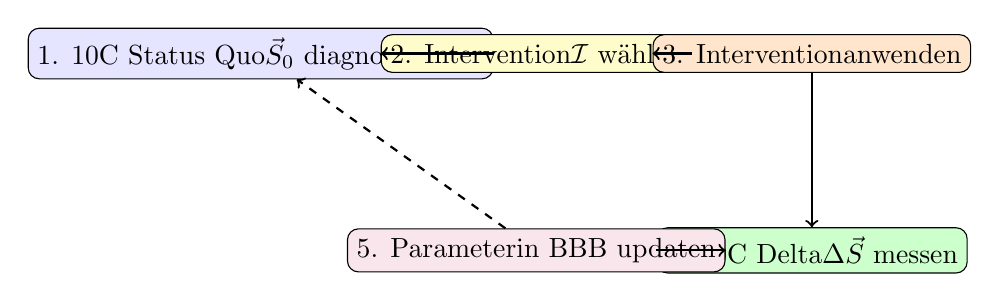
\begin{tikzpicture}[node distance=2.5cm, auto]
\node[draw, rounded corners, fill=blue!10, minimum width=3.5cm] (diag) {1. 10C Status Quo\\$\vec{S}_0$ diagnostizieren};
\node[draw, rounded corners, fill=yellow!20, minimum width=3.5cm, right of=diag, xshift=1cm] (select) {2. Intervention\\$\mathcal{I}$ wählen};
\node[draw, rounded corners, fill=orange!20, minimum width=3.5cm, right of=select, xshift=1cm] (apply) {3. Intervention\\anwenden};
\node[draw, rounded corners, fill=green!20, minimum width=3.5cm, below of=apply] (measure) {4. 10C Delta\\$\Delta\vec{S}$ messen};
\node[draw, rounded corners, fill=purple!10, minimum width=3.5cm, left of=measure, xshift=-1cm] (learn) {5. Parameter\\in BBB updaten};

\draw[->, thick] (diag) -- (select);
\draw[->, thick] (select) -- (apply);
\draw[->, thick] (apply) -- (measure);
\draw[->, thick] (measure) -- (learn);
\draw[->, thick, dashed] (learn) -- (diag);
\end{tikzpicture}
\end{center}

\textbf{Feedback into 10C System:}
\begin{enumerate}[nosep]
\item $\Delta A, \Delta W$: Updates for $A(\cdot)$ and $W_{\text{eff}}$ models (AU, AV)
\item $\Delta\gamma$: New complementarity estimates $\rightarrow$ HOW (B)
\item $\Delta\Theta$: Parameter Repository (BBB) updated
\item $\Delta\varphi$: Journey transition probabilities (AW) refined
\end{enumerate}
\end{tcolorbox}

\subsection{10C Delta Measurement Protocol}

\begin{table}[htbp]
\centering
\caption{10C Delta Measurement: Dimensions, Metrics, and Primary Intervention Type}
\label{tab:hhh-9c-delta-measurement}
\renewcommand{\arraystretch}{1.4}
\footnotesize
\begin{tabular}{@{}llp{4.5cm}l@{}}
\toprule
\textbf{CORE} & \textbf{$\Delta$} & \textbf{Measurement Method} & \textbf{Primary Type} \\
\midrule
\textbf{WHO} (AAA) & $\Delta L$ & Shift in Welfare-Level (L1→L2→L3→L4) & T5, T6 \\
\textbf{WHAT} (C) & $\Delta d$ & Change in FEPSDE weighting & T5, T7 \\
\textbf{HOW} (B) & $\Delta\gamma$ & New complementarities activated & T8, T3 \\
\textbf{WHEN} (V) & $\Delta\Psi$ & Context sensitivity changed & T3, T4 \\
\textbf{WHERE} (BBB) & $\Delta\Theta$ & Parameter updates (Bayesian) & All \\
\textbf{AWARE} (AU) & $\Delta A$ & $A_1 - A_0$ (0--1 scale) & T1, T2 \\
\textbf{READY} (AV) & $\Delta W$ & $W_{\text{eff},1} - W_{\text{eff},0}$ & T2, T4 \\
\textbf{STAGE} (AW) & $\Delta\varphi$ & Journey phase progression & T3, T4 \\
\textbf{HIERARCHY} (HI) & $\Delta$Scope & Instant→Identity→Habit shift & T5, T8 \\
\bottomrule
\end{tabular}
\end{table}

\begin{tcolorbox}[colback=gray!5!white, colframe=gray!75!black,
    title=Definition HHH-D0b: Portfolio Success Criteria]
\begin{equation}
\text{Portfolio Success} = \begin{cases}
\text{Full} & \text{if } \Delta A > 0, \Delta W > 0, \Delta\varphi \geq 0 \\
\text{Partial} & \text{if at least 2 of 3 positive} \\
\text{Failed} & \text{if } \Delta A \leq 0 \text{ and } \Delta W \leq 0
\end{cases}
\end{equation}
\end{tcolorbox}


%%%%%%%%%%%%%%%%%%%%%%%%%%%%%%%%%%%%%%%%%%%%%%%%%%%%%%%%%%%%%%%%%%%%%%%%%%%%%%%
\section{Core Theory: The 20-Field Intervention Schema}
\label{sec:hhh-theory}
%%%%%%%%%%%%%%%%%%%%%%%%%%%%%%%%%%%%%%%%%%%%%%%%%%%%%%%%%%%%%%%%%%%%%%%%%%%%%%%

\subsection{Application Depth Modes}

The toolkit supports three application depths, allowing progressive refinement:

\begin{table}[htbp]
\centering
\caption{Application Depth Levels}
\label{tab:hhh-depths}
\renewcommand{\arraystretch}{1.3}
\begin{tabular}{@{}clll@{}}
\toprule
\textbf{Iteration} & \textbf{Mode} & \textbf{Fields Activated} & \textbf{Use Case} \\
\midrule
1 & Light & F1--F6 & Rapid prototyping, initial screening \\
2 & Hybrid & F1--F12 & Standard intervention design \\
3 & Profound & F1--F18 (F19--F20 optional) & Full specification, research-grade \\
\bottomrule
\end{tabular}
\end{table}

\subsection{The Complete Field Structure}

\begin{table}[htbp]
\centering
\caption{Complete 20-Field Intervention Schema}
\label{tab:hhh-fields}
\renewcommand{\arraystretch}{1.2}
\small
\begin{tabular}{@{}clllp{4.5cm}@{}}
\toprule
\textbf{ID} & \textbf{Field Name} & \textbf{Type} & \textbf{Required} & \textbf{Description} \\
\midrule
\multicolumn{5}{@{}l}{\textit{\textbf{Light Mode (F1--F6)}}} \\
F1 & Title/Label & Text & Light & Clear name of the intervention \\
F2 & Intervention Type & Choice & Light & One of 8 primitive types (see Table~\ref{tab:hhh-types-derived}) \\
F3 & Context Level & Choice & Light & State, Organization, Individual, etc. \\
F4 & Target Structure & Multi & Light & IND/IDN/Collective utility targets \\
F5 & FEPSDE Dimension & Multi & Light & Financial/Emotional/Physical/Social/Digital/Ecological \\
F6 & Journey Phase & Choice & Light & Awareness, Trigger, Stabilization (from AW) \\
\addlinespace
\multicolumn{5}{@{}l}{\textit{\textbf{Hybrid Mode (F7--F12)}}} \\
F7 & Framing Logic & Choice & Hybrid & Positive/Negative/Social/Neutral \\
F8 & Autonomy Level & Choice & Hybrid & Voluntary, Default, Mandate, Prohibition \\
F9 & Target Segment & ID & Hybrid & Link to segment (from BA) \\
F10 & Complementarity & Ref-List & Hybrid & Links to other interventions \\
F11 & Side Effect Risk & Choice+Text & Hybrid & Low/Medium/High + explanation \\
F12 & Temporal Scope & Choice & Hybrid & Instant/Operative/Tactical/Strategic/System (from HHH-T2) \\
\addlinespace
\multicolumn{5}{@{}l}{\textit{\textbf{Profound Mode (F13--F18)}}} \\
F13 & Evaluation Plan & Choice & Profound & Yes/No + evaluation form \\
F14 & Path Function & Choice & Profound & Door-opener/Amplifier/Escalator/Stabilizer \\
F15 & Repetition Required & Choice & Profound & Yes/No/Cyclic \\
F16 & Responsible Role & Text & Profound & HR, Policy, School, Parents, etc. \\
F17 & Source/Evidence & Text/Link & Profound & Studies, literature, pilot projects \\
F18 & System Link/ID & Code & Profound & Internal ID or API reference \\
\addlinespace
\multicolumn{5}{@{}l}{\textit{\textbf{Optional (F19--F20)}}} \\
F19 & Description & Long Text & Optional & Explanation of mechanism \\
F20 & Status/Validation & Choice & Optional & Planned/Tested/Active/Rejected \\
\bottomrule
\end{tabular}
\end{table}

\subsection{Theoretical Derivation of Intervention Types (F2)}
\label{sec:hhh-types}

\begin{tcolorbox}[colback=blue!5!white, colframe=blue!75!black,
    title=\textbf{Theorem HHH-T1: Intervention Type Emergence}]

\textbf{Statement:} Intervention types emerge from the structure of the Effective Willingness function. Given:
\begin{equation}
W_{\text{eff}} = W_{\text{base}} \cdot A(\cdot) \cdot (1 + \kappa_{AWX}) \cdot (1 + \kappa_{KON}) \cdot (1 + \kappa_{JNY})
\label{eq:hhh-weff}
\end{equation}

An intervention $\mathcal{I}$ is a mapping that modifies one or more components:
\begin{equation}
\mathcal{I}: (W_{\text{base}}, A, \kappa_{AWX}, \kappa_{KON}, \kappa_{JNY}, u_d) \mapsto (W'_{\text{base}}, A', \kappa'_{AWX}, \kappa'_{KON}, \kappa'_{JNY}, u'_d)
\end{equation}

\textbf{Corollary:} There exist exactly 8 primitive intervention types, each targeting a distinct component:
\end{tcolorbox}

\begin{table}[htbp]
\centering
\caption{Theoretically Derived Intervention Types}
\label{tab:hhh-types-derived}
\renewcommand{\arraystretch}{1.3}
\begin{tabular}{@{}clllp{3.5cm}@{}}
\toprule
\textbf{\#} & \textbf{Type} & \textbf{Target} & \textbf{Formal} & \textbf{Literature Name} \\
\midrule
1 & Awareness & $A(\cdot)$ & $A \mapsto A'$ & Informative \\
2 & Feedback & $\kappa_{AWX}$ & $\kappa_{AWX} \mapsto \kappa'_{AWX}$ & Feedback-based \\
3 & Contextual & $\kappa_{KON}$ & $\kappa_{KON} \mapsto \kappa'_{KON}$ & Structural/Nudge \\
4 & Temporal & $\kappa_{JNY}$ & $\kappa_{JNY} \mapsto \kappa'_{JNY}$ & Temporal \\
5 & Identity & $W_{\text{base}}$ & $W_{\text{base}} \mapsto W'_{\text{base}}$ & Identity-based \\
6 & Social & $u_S$ & $u_S \mapsto u'_S$ & Normative \\
7 & Financial & $u_F$ & $u_F \mapsto u'_F$ & Incentive-based \\
8 & Binding & $\gamma_{ij}$ & $\gamma_{ij} \mapsto \gamma'_{ij}$ & Commitment \\
\bottomrule
\end{tabular}
\end{table}

\begin{tcolorbox}[colback=gray!5!white, colframe=gray!75!black,
    title=Definition HHH-D1: Hybrid Interventions]
\textbf{Definition:} A \textit{hybrid intervention} $\mathcal{I}_H$ modifies multiple components simultaneously:
\begin{equation}
\mathcal{I}_H = \mathcal{I}_1 \circ \mathcal{I}_2 \circ \ldots \circ \mathcal{I}_k \quad \text{where } k \geq 2
\end{equation}

\textbf{Note:} Hybrid interventions are \textit{not} a primitive type but compositions of primitive types. Their effectiveness depends on complementarity:
\begin{equation}
E(\mathcal{I}_H) = \sum_{i} E(\mathcal{I}_i) + \sum_{i < j} \gamma_{ij} \cdot \sqrt{E(\mathcal{I}_i) \cdot E(\mathcal{I}_j)}
\end{equation}
\end{tcolorbox}

\begin{tcolorbox}[colback=red!5!white, colframe=red!75!black,
    title=\textbf{Methodological Note: XVIII Exclusion Principle for Types}]
Following Appendix UNMAPPED_FRM, the 8 primitive types represent \textbf{single-mechanism interventions}. The burden of proof lies with hybrid interventions:

\begin{itemize}[nosep]
    \item \textbf{Null hypothesis:} Single-mechanism interventions are sufficient
    \item \textbf{Alternative:} Multi-mechanism (hybrid) intervention required
    \item \textbf{Test:} Only combine if single mechanisms demonstrably fail
\end{itemize}

\textit{Intervention bundling must be empirically justified, not assumed.}
\end{tcolorbox}


\subsection{Theoretical Derivation of Temporal Scope (F12)}
\label{sec:hhh-temporal}

\begin{tcolorbox}[colback=blue!5!white, colframe=blue!75!black,
    title=\textbf{Theorem HHH-T2: Temporal Scope Emergence from HIERARCHY}]

\textbf{Statement:} The temporal scope of an intervention emerges from the decision level it targets in the HIERARCHY (HI) framework.

\textbf{Given:} The HIERARCHY stratification (Appendix UNMAPPED_HIE, Chapter 15):
\begin{itemize}[nosep]
    \item \textbf{L0 (Meta):} Scope-defining decisions --- ``What counts as a decision?''
    \item \textbf{L1 (Strategic Roots):} Few decisions with high interaction ($\gamma$ high)
    \item \textbf{L2 (Derived Strategic):} Decisions relational to L1
    \item \textbf{L3 (Operative):} Many decisions with low interaction ($\gamma \approx 0$)
\end{itemize}

\textbf{Derivation:} An intervention's temporal scope $\mathcal{T}(\mathcal{I})$ is determined by its target decision level:
\begin{equation}
\mathcal{T}(\mathcal{I}) = f(L_{\text{target}}) \quad \text{where } L_{\text{target}} \in \{L0, L1, L2, L3\}
\label{eq:hhh-temporal-mapping}
\end{equation}

\textbf{Corollary:} The mapping is monotonic in strategic relevance:
\begin{equation}
L_{\text{target}} \downarrow \; \Rightarrow \; \mathcal{T}(\mathcal{I}) \downarrow \quad \text{(lower level = shorter scope)}
\end{equation}

\end{tcolorbox}

\begin{table}[htbp]
\centering
\caption{Theoretically Derived Temporal Scope Categories}
\label{tab:hhh-temporal-derived}
\renewcommand{\arraystretch}{1.3}
\begin{tabular}{@{}cllcp{4cm}@{}}
\toprule
\textbf{Level} & \textbf{Scope} & \textbf{Target} & \textbf{Horizon} & \textbf{Example} \\
\midrule
L3 & Instant & Operative decisions & Hours--Days & Real-time feedback, alerts \\
L3 & Operative & Routine behaviors & Days--Weeks & Nudges, defaults, prompts \\
L2 & Tactical & Derived strategies & Weeks--Months & Programs, campaigns \\
L1 & Strategic & Root strategies & Months--Years & Policy changes, incentive structures \\
L0 & System & Scope definitions & Years--Decades & Regulatory frameworks, norms \\
\bottomrule
\end{tabular}
\end{table}

\begin{tcolorbox}[colback=gray!5!white, colframe=gray!75!black,
    title=Definition HHH-D2: Temporal Scope Categories]

\textbf{Definition:} The five temporal scope categories for F12 are:

\begin{enumerate}[nosep]
    \item \textbf{Instant} ($\mathcal{T}_I$): Targets L3 decisions with immediate effect. Effect decays within hours to days unless reinforced.
    \begin{equation}
    \tau_{\text{decay}}(\mathcal{T}_I) \in [1\text{h}, 7\text{d}]
    \end{equation}

    \item \textbf{Operative} ($\mathcal{T}_O$): Targets L3 routines with short-term effect. Effect decays within days to weeks.
    \begin{equation}
    \tau_{\text{decay}}(\mathcal{T}_O) \in [1\text{d}, 4\text{w}]
    \end{equation}

    \item \textbf{Tactical} ($\mathcal{T}_T$): Targets L2 derived decisions. Effect persists weeks to months.
    \begin{equation}
    \tau_{\text{decay}}(\mathcal{T}_T) \in [1\text{w}, 6\text{m}]
    \end{equation}

    \item \textbf{Strategic} ($\mathcal{T}_S$): Targets L1 root decisions. Effect persists months to years.
    \begin{equation}
    \tau_{\text{decay}}(\mathcal{T}_S) \in [1\text{m}, 5\text{y}]
    \end{equation}

    \item \textbf{System} ($\mathcal{T}_{Sy}$): Targets L0 scope definitions. Effect persists years to decades.
    \begin{equation}
    \tau_{\text{decay}}(\mathcal{T}_{Sy}) \in [1\text{y}, \infty]
    \end{equation}
\end{enumerate}

\end{tcolorbox}

\begin{tcolorbox}[colback=orange!5!white, colframe=orange!75!black,
    title=\textbf{The Two-Dimensional Intervention Classification}]

\textbf{Result:} Combining Theorems HHH-T1 and HHH-T2, every intervention $\mathcal{I}$ is classified along two orthogonal dimensions:

\begin{equation}
\boxed{\mathcal{I} \mapsto (\text{Type}, \text{Scope}) \in \{1, \ldots, 8\} \times \{I, O, T, S, Sy\}}
\label{eq:hhh-2d-classification}
\end{equation}

\textbf{Type} (from HHH-T1): \textit{Which component of $W_{\text{eff}}$ is targeted?}
\begin{itemize}[nosep]
    \item 8 primitive types: Awareness, Feedback, Contextual, Temporal, Identity, Social, Financial, Binding
\end{itemize}

\textbf{Scope} (from HHH-T2): \textit{Which decision level is targeted?}
\begin{itemize}[nosep]
    \item 5 scopes: Instant (L3), Operative (L3), Tactical (L2), Strategic (L1), System (L0)
\end{itemize}

\textbf{Implication:} The intervention design space has $8 \times 5 = 40$ cells, each representing a distinct intervention archetype.

\end{tcolorbox}

\begin{table}[htbp]
\centering
\caption{The 8×5 Intervention Classification Matrix (Selected Examples)}
\label{tab:hhh-matrix}
\renewcommand{\arraystretch}{1.2}
\small
\begin{tabular}{@{}l|ccccc@{}}
\toprule
\textbf{Type $\backslash$ Scope} & \textbf{Instant} & \textbf{Operative} & \textbf{Tactical} & \textbf{Strategic} & \textbf{System} \\
\midrule
Awareness & Alert & Daily email & Campaign & Curriculum & Media norms \\
Feedback & Real-time & Weekly report & Quarterly review & Annual eval & Rating systems \\
Contextual & Pop-up & Default & Program design & Policy design & Regulatory \\
Temporal & Reminder & Scheduling & Planning tools & Life planning & Pension rules \\
Identity & Moment prime & Daily affirmation & Role transition & Career identity & Cultural identity \\
Social & Social cue & Peer group & Network program & Community & Social norms \\
Financial & Micro-reward & Bonus & Incentive program & Tax structure & Economic policy \\
Binding & Commitment & Contract & Goal system & Institutional & Legal binding \\
\bottomrule
\end{tabular}
\end{table}

\begin{tcolorbox}[colback=red!5!white, colframe=red!75!black,
    title=\textbf{Methodological Note: XVIII Exclusion Principle for Scope}]

Following Appendix UNMAPPED_FRM, the temporal scope classification implies:

\begin{itemize}[nosep]
    \item \textbf{Null hypothesis for scope:} Target the lowest sufficient decision level (L3 first)
    \item \textbf{Escalation justified:} Move to higher levels (L2, L1, L0) only when lower-level interventions demonstrably fail
    \item \textbf{Parsimony:} Instant interventions are preferred to Strategic interventions when both achieve the same outcome
\end{itemize}

\textbf{Rationale:} Lower-level interventions are:
\begin{enumerate}[nosep]
    \item Faster to implement and evaluate
    \item Less costly (lower coordination requirements)
    \item More reversible if ineffective
    \item Less disruptive to existing systems
\end{enumerate}

\textit{Intervention scope should be as low as effective, not as high as possible.}
\end{tcolorbox}


\subsection{Theoretical Derivation of Target Level (F4)}
\label{sec:hhh-level}

\begin{tcolorbox}[colback=blue!5!white, colframe=blue!75!black,
    title=\textbf{Theorem HHH-T3: Target Level Emergence from WHO}]

\textbf{Statement:} The welfare target level of an intervention emerges from the WHO framework (Appendix UNMAPPED_WHO).

\textbf{Given:} The Welfare Hierarchy levels:
\begin{itemize}[nosep]
    \item \textbf{L1 (Individual):} Single agent utility $U^1_i$
    \item \textbf{L2 (Dyadic):} Two-agent interactions $U^2_{ij}$
    \item \textbf{L3 (Group):} Collective utility $U^3_G$
    \item \textbf{L4 (Societal):} Population-level welfare $U^4_S$
\end{itemize}

\textbf{Derivation:} An intervention's target level $\mathcal{L}(\mathcal{I})$ is determined by its welfare impact scope:
\begin{equation}
\mathcal{L}(\mathcal{I}) = \max\{ L : \frac{\partial E(\mathcal{I})}{\partial U^L} \neq 0 \}
\label{eq:hhh-level-mapping}
\end{equation}

\textbf{Corollary:} Interventions targeting higher levels require coordination across lower levels:
\begin{equation}
\mathcal{L} = k \Rightarrow \text{Coordination}(\mathcal{I}) \propto \prod_{l=1}^{k} n_l
\end{equation}

\end{tcolorbox}

\begin{table}[htbp]
\centering
\caption{Theoretically Derived Target Level Categories (F4)}
\label{tab:hhh-level-derived}
\renewcommand{\arraystretch}{1.3}
\begin{tabular}{@{}cllp{4.5cm}@{}}
\toprule
\textbf{Level} & \textbf{Target} & \textbf{Coordination} & \textbf{Example Intervention} \\
\midrule
L1 & Individual & None & Personal reminder, self-commitment \\
L2 & Dyadic & Bilateral & Couples counseling, mentorship \\
L3 & Group & Multilateral & Team incentives, organizational policy \\
L4 & Societal & Institutional & Tax policy, regulatory framework \\
\bottomrule
\end{tabular}
\end{table}


\subsection{Theoretical Derivation of Utility Dimension (F5)}
\label{sec:hhh-dimension}

\begin{tcolorbox}[colback=blue!5!white, colframe=blue!75!black,
    title=\textbf{Theorem HHH-T4: Utility Dimension Emergence from WHAT}]

\textbf{Statement:} The utility dimension targeted by an intervention emerges from the FEPSDE framework (Appendix UNMAPPED_WAT/CORE-WHAT).

\textbf{Given:} The six utility dimensions:
\begin{equation}
U = \sum_{d \in \text{FEPSDE}} \omega_d \cdot u_d \quad \text{where FEPSDE} = \{F, E, P, S, D, X\}
\end{equation}

\textbf{Derivation:} An intervention's primary dimension $d^*(\mathcal{I})$ is:
\begin{equation}
d^*(\mathcal{I}) = \arg\max_{d \in \text{FEPSDE}} \left| \frac{\partial E(\mathcal{I})}{\partial u_d} \right|
\label{eq:hhh-dimension-mapping}
\end{equation}

\textbf{Multi-dimensional interventions:} Some interventions affect multiple dimensions simultaneously. Define the dimension vector:
\begin{equation}
\vec{d}(\mathcal{I}) = \left( \frac{\partial E}{\partial u_F}, \frac{\partial E}{\partial u_E}, \frac{\partial E}{\partial u_P}, \frac{\partial E}{\partial u_S}, \frac{\partial E}{\partial u_D}, \frac{\partial E}{\partial u_X} \right)
\end{equation}

\end{tcolorbox}

\begin{table}[htbp]
\centering
\caption{Theoretically Derived Utility Dimension Categories (F5)}
\label{tab:hhh-dimension-derived}
\renewcommand{\arraystretch}{1.3}
\begin{tabular}{@{}clp{5cm}p{3.5cm}@{}}
\toprule
\textbf{Code} & \textbf{Dimension} & \textbf{Target Utility} & \textbf{Example} \\
\midrule
F & Financial & Monetary outcomes, wealth & Incentives, subsidies \\
E & Emotional & Affective states, well-being & Framing, messaging \\
P & Physical & Health, bodily states & Health nudges, defaults \\
S & Social & Relationships, status, norms & Social proof, peer effects \\
D & Development & Learning, growth, skills & Training, education \\
X & Existential & Meaning, purpose, identity & Values-based appeals \\
\bottomrule
\end{tabular}
\end{table}


\subsection{Theoretical Derivation of Journey Phase (F6)}
\label{sec:hhh-phase}

\begin{tcolorbox}[colback=blue!5!white, colframe=blue!75!black,
    title=\textbf{Theorem HHH-T5: Journey Phase Emergence from STAGE}]

\textbf{Statement:} The optimal journey phase for an intervention emerges from the Behavioral Change Journey (Appendix UNMAPPED_STA/CORE-STAGE).

\textbf{Given:} The BCJ state variable $S(t) \in [0, 1]$ with five phases:
\begin{equation}
\varphi(S) = \begin{cases}
1 \text{ (Awareness)} & S \in [0, 0.2) \\
2 \text{ (Trigger)} & S \in [0.2, 0.4) \\
3 \text{ (Action)} & S \in [0.4, 0.6) \\
4 \text{ (Maintenance)} & S \in [0.6, 0.8) \\
5 \text{ (Stabilization)} & S \in [0.8, 1.0]
\end{cases}
\end{equation}

\textbf{Derivation:} Each intervention type (from HHH-T1) has maximal effectiveness in specific phases:
\begin{equation}
\varphi^*(\mathcal{I}) = \arg\max_{\varphi} E(\mathcal{I} | \varphi)
\label{eq:hhh-phase-mapping}
\end{equation}

\textbf{Phase-Type Affinity Matrix:} Define $\alpha_{t\varphi} \in [0,1]$ as the affinity of type $t$ for phase $\varphi$.

\end{tcolorbox}

\begin{table}[htbp]
\centering
\caption{Type-Phase Affinity Matrix (HHH-T5)}
\label{tab:hhh-phase-affinity}
\renewcommand{\arraystretch}{1.2}
\small
\begin{tabular}{@{}l|ccccc@{}}
\toprule
\textbf{Type} & \textbf{Aware} & \textbf{Trigger} & \textbf{Action} & \textbf{Maint.} & \textbf{Stabil.} \\
\midrule
Awareness & \textbf{1.0} & 0.6 & 0.2 & 0.1 & 0.1 \\
Feedback & 0.3 & 0.5 & \textbf{0.9} & 0.8 & 0.6 \\
Contextual & 0.2 & \textbf{0.9} & 0.8 & 0.5 & 0.3 \\
Temporal & 0.4 & 0.6 & 0.7 & \textbf{0.8} & 0.7 \\
Identity & 0.5 & 0.4 & 0.5 & 0.7 & \textbf{0.9} \\
Social & 0.6 & 0.7 & \textbf{0.8} & 0.7 & 0.6 \\
Financial & 0.2 & \textbf{0.8} & 0.7 & 0.4 & 0.2 \\
Binding & 0.1 & 0.5 & 0.6 & \textbf{0.9} & 0.8 \\
\bottomrule
\end{tabular}
\end{table}


\subsection{Theoretical Derivation of Awareness Regime (NEW)}
\label{sec:hhh-awareness}

\begin{tcolorbox}[colback=blue!5!white, colframe=blue!75!black,
    title=\textbf{Theorem HHH-T6: Awareness Regime Emergence from AWARE}]

\textbf{Statement:} The effectiveness of an intervention depends on the target population's awareness state (Appendix UNMAPPED_AWA/CORE-AWARE).

\textbf{Given:} The Awareness function $A(t^*) \in [0, 1]$ filtering potential to effective utility:
\begin{equation}
U^{\text{eff}} = A(t^*) \cdot U^{\text{pot}}
\end{equation}

\textbf{Derivation:} Define three awareness regimes:
\begin{equation}
\mathcal{A}(\text{target}) = \begin{cases}
\text{Unaware} & A < 0.3 \\
\text{Partial} & A \in [0.3, 0.7] \\
\text{Full} & A > 0.7
\end{cases}
\label{eq:hhh-awareness-regime}
\end{equation}

\textbf{Intervention-Awareness Interaction:}
\begin{equation}
E(\mathcal{I} | \mathcal{A}) = E_0(\mathcal{I}) \cdot g(\mathcal{A}, \text{Type}(\mathcal{I}))
\end{equation}

where $g$ is the awareness-type interaction function.

\end{tcolorbox}

\begin{table}[htbp]
\centering
\caption{Type-Awareness Effectiveness Matrix (HHH-T6)}
\label{tab:hhh-awareness-matrix}
\renewcommand{\arraystretch}{1.2}
\begin{tabular}{@{}l|ccc@{}}
\toprule
\textbf{Type} & \textbf{Unaware} & \textbf{Partial} & \textbf{Full} \\
\midrule
Awareness & \textbf{High} & Medium & Low (redundant) \\
Feedback & Low & \textbf{High} & Medium \\
Contextual & \textbf{High} & High & Medium \\
Temporal & Low & Medium & \textbf{High} \\
Identity & Low & Medium & \textbf{High} \\
Social & Medium & \textbf{High} & Medium \\
Financial & Medium & \textbf{High} & High \\
Binding & Low & Medium & \textbf{High} \\
\bottomrule
\end{tabular}
\end{table}


\subsection{The Complete Multi-Dimensional Classification}
\label{sec:hhh-complete}

\begin{tcolorbox}[colback=green!5!white, colframe=green!75!black,
    title=\textbf{Theorem HHH-T7: Complete Intervention Classification Space}]

\textbf{Statement:} Combining Theorems HHH-T1 through HHH-T6, every intervention is fully classified by a 6-dimensional vector:

\begin{equation}
\boxed{\mathcal{I} \mapsto (\text{Type}, \text{Scope}, \text{Level}, \text{Dimension}, \text{Phase}, \text{Awareness})}
\label{eq:hhh-6d-classification}
\end{equation}

\textbf{Dimension Cardinalities:}
\begin{itemize}[nosep]
    \item \textbf{Type} (HHH-T1): 8 categories (from $W_{\text{eff}}$)
    \item \textbf{Scope} (HHH-T2): 5 categories (from HIERARCHY)
    \item \textbf{Level} (HHH-T3): 4 categories (from WHO)
    \item \textbf{Dimension} (HHH-T4): 6 categories (from WHAT/FEPSDE)
    \item \textbf{Phase} (HHH-T5): 5 categories (from STAGE)
    \item \textbf{Awareness} (HHH-T6): 3 categories (from AWARE)
\end{itemize}

\textbf{Theoretical Space:} $8 \times 5 \times 4 \times 6 \times 5 \times 3 = 14{,}400$ intervention archetypes.

\textbf{Practical Reduction:} Many combinations are infeasible or redundant. The affinity matrices (Tables~\ref{tab:hhh-phase-affinity}, \ref{tab:hhh-awareness-matrix}) constrain the effective design space.

\end{tcolorbox}

\begin{tcolorbox}[colback=orange!5!white, colframe=orange!75!black,
    title=\textbf{Field Mapping: 6D Classification to 20-Field Schema}]

The 6 theoretical dimensions map directly to existing fields:

\begin{center}
\begin{tabular}{@{}lll@{}}
\toprule
\textbf{Theorem} & \textbf{Dimension} & \textbf{Field} \\
\midrule
HHH-T1 & Type & F2 (Intervention Type) \\
HHH-T2 & Scope & F12 (Temporal Scope) \\
HHH-T3 & Level & F4 (Target Structure) \\
HHH-T4 & Dimension & F5 (FEPSDE Dimension) \\
HHH-T5 & Phase & F6 (Journey Phase) \\
HHH-T6 & Awareness & \textit{NEW: F21 proposed} \\
\bottomrule
\end{tabular}
\end{center}

\textbf{Note:} Awareness regime (HHH-T6) suggests extending the schema to 21 fields, or incorporating it into F6 (Journey Phase) as a sub-classification.

\end{tcolorbox}

\begin{tcolorbox}[colback=red!5!white, colframe=red!75!black,
    title=\textbf{Methodological Note: XVIII Exclusion Principle for All Dimensions}]

Following Appendix UNMAPPED_FRM, the multi-dimensional classification implies a hierarchy of parsimony:

\begin{enumerate}[nosep]
    \item \textbf{Type:} Single-mechanism before hybrid
    \item \textbf{Scope:} Lowest level (Instant) before highest (System)
    \item \textbf{Level:} Individual (L1) before Societal (L4)
    \item \textbf{Dimension:} Single FEPSDE dimension before multi-dimensional
    \item \textbf{Phase:} Match actual phase, don't assume
    \item \textbf{Awareness:} Diagnose before intervening
\end{enumerate}

\textbf{The Parsimony Principle:}
\begin{equation}
\text{Preferred}(\mathcal{I}_1, \mathcal{I}_2) = \mathcal{I}_1 \quad \text{if } \|\vec{d}(\mathcal{I}_1)\|_0 < \|\vec{d}(\mathcal{I}_2)\|_0 \text{ and } E(\mathcal{I}_1) \approx E(\mathcal{I}_2)
\end{equation}

\textit{Simpler interventions are preferred when effectiveness is comparable.}
\end{tcolorbox}


\subsection{Feasibility Reduction: From 14,400 to Practical Space}
\label{sec:hhh-reduction}

\begin{tcolorbox}[colback=blue!5!white, colframe=blue!75!black,
    title=\textbf{Theorem HHH-T8: Feasibility Constraint System}]

\textbf{Problem:} The theoretical space of $8 \times 5 \times 4 \times 6 \times 5 \times 3 = 14{,}400$ archetypes is impractical. We need a principled method to reduce to feasible interventions.

\textbf{Statement:} An intervention archetype $\vec{a} = (t, s, l, d, \varphi, A)$ is \textbf{feasible} if and only if it satisfies all constraint classes:
\begin{equation}
\boxed{\text{Feasible}(\vec{a}) \iff C_{\text{affinity}}(\vec{a}) \wedge C_{\text{logical}}(\vec{a}) \wedge C_{\text{scale}}(\vec{a}) \wedge C_{\text{empirical}}(\vec{a})}
\label{eq:hhh-feasibility}
\end{equation}

\end{tcolorbox}

\begin{tcolorbox}[colback=gray!5!white, colframe=gray!75!black,
    title=Definition HHH-D3: Four Constraint Classes]

\textbf{Class 1: Affinity Constraints} $C_{\text{affinity}}$

An archetype fails affinity if interaction strength is below threshold:
\begin{equation}
C_{\text{affinity}}(\vec{a}) \iff \alpha_{t,\varphi} \geq \theta_\alpha \wedge g(A, t) \neq \text{``Low''}
\end{equation}
where $\theta_\alpha = 0.4$ (from Tables~\ref{tab:hhh-phase-affinity}, \ref{tab:hhh-awareness-matrix}).

\textbf{Pruning effect:} Eliminates combinations where Type-Phase or Type-Awareness affinity is weak.

\medskip
\textbf{Class 2: Logical Constraints} $C_{\text{logical}}$

Some combinations are logically contradictory:
\begin{align}
C_{\text{logical}}(\vec{a}) \iff &\neg(\varphi = \text{Awareness} \wedge A = \text{Full}) \tag{Redundancy} \\
&\wedge \neg(t = \text{Awareness} \wedge A = \text{Full}) \tag{Type-Awareness} \\
&\wedge \neg(s = \text{System} \wedge l = \text{Individual}) \tag{Scale mismatch}
\end{align}

\textbf{Pruning effect:} Eliminates self-contradictory archetypes.

\medskip
\textbf{Class 3: Scale Consistency Constraints} $C_{\text{scale}}$

Scope and Level must be coherent:
\begin{equation}
C_{\text{scale}}(\vec{a}) \iff |s_{\text{rank}} - l_{\text{rank}}| \leq 2
\end{equation}
where ranks are: Instant=1, Operative=2, Tactical=3, Strategic=4, System=5 for Scope; Individual=1, Dyadic=2, Group=3, Societal=4 for Level.

\textbf{Pruning effect:} Individual-level interventions cannot have System scope; Societal-level cannot be Instant.

\medskip
\textbf{Class 4: Empirical Constraints} $C_{\text{empirical}}$

Some combinations have no evidence base:
\begin{equation}
C_{\text{empirical}}(\vec{a}) \iff \exists \text{ literature support for } (t, d) \text{ pairing}
\end{equation}

\textbf{Pruning effect:} Eliminates Type-Dimension combinations with no theoretical or empirical foundation.

\end{tcolorbox}

\begin{tcolorbox}[colback=orange!5!white, colframe=orange!75!black,
    title=\textbf{Algorithm HHH-A1: Feasibility Pruning}]

\textbf{Input:} Full archetype space $\mathcal{A} = \{1,...,8\} \times \{1,...,5\} \times \{1,...,4\} \times \{1,...,6\} \times \{1,...,5\} \times \{1,...,3\}$

\textbf{Output:} Feasible archetype space $\mathcal{A}^*$

\begin{verbatim}
ALGORITHM Prune-Archetypes:
  A* = {}
  FOR each archetype a = (t, s, l, d, φ, A) in A:

    # Step 1: Affinity check
    IF α[t,φ] < 0.4: CONTINUE
    IF g[A,t] == "Low": CONTINUE

    # Step 2: Logical check
    IF (φ == Awareness AND A == Full): CONTINUE
    IF (t == Awareness AND A == Full): CONTINUE
    IF (s == System AND l == Individual): CONTINUE

    # Step 3: Scale consistency
    IF |rank(s) - rank(l)| > 2: CONTINUE

    # Step 4: Empirical support (lookup table)
    IF NOT empirical_support[t,d]: CONTINUE

    # Passed all constraints
    A*.add(a)

  RETURN A*
\end{verbatim}

\end{tcolorbox}

\begin{tcolorbox}[colback=green!5!white, colframe=green!75!black,
    title=\textbf{Result: Estimated Feasible Space Size}]

\textbf{Reduction Analysis:}

\begin{table}[H]
\centering
\begin{tabular}{@{}lrrl@{}}
\toprule
\textbf{Constraint Class} & \textbf{Reduction} & \textbf{Remaining} & \textbf{Mechanism} \\
\midrule
Starting space & -- & 14,400 & Full combinatorial \\
$C_{\text{affinity}}$ (Phase) & $\sim 40\%$ & 8,640 & Low $\alpha_{t\varphi}$ eliminated \\
$C_{\text{affinity}}$ (Awareness) & $\sim 25\%$ & 6,480 & ``Low'' effectiveness eliminated \\
$C_{\text{logical}}$ & $\sim 10\%$ & 5,832 & Contradictions removed \\
$C_{\text{scale}}$ & $\sim 30\%$ & 4,082 & Scale mismatches removed \\
$C_{\text{empirical}}$ & $\sim 50\%$ & 2,041 & No evidence combinations removed \\
\midrule
\textbf{Final estimate} & $\sim 86\%$ & $\sim 2{,}000$ & \textbf{Practical archetypes} \\
\bottomrule
\end{tabular}
\end{table}

\textbf{Interpretation:} Only $\sim 14\%$ of the theoretical space represents feasible interventions. The practical design space has approximately \textbf{2,000 intervention archetypes}.

\end{tcolorbox}

\begin{table}[htbp]
\centering
\caption{Type-Dimension Empirical Support Matrix (for $C_{\text{empirical}}$)}
\label{tab:hhh-type-dimension}
\renewcommand{\arraystretch}{1.2}
\small
\begin{tabular}{@{}l|cccccc@{}}
\toprule
\textbf{Type $\backslash$ Dim} & \textbf{F} & \textbf{E} & \textbf{P} & \textbf{S} & \textbf{D} & \textbf{X} \\
\midrule
Awareness & \checkmark & \checkmark & \checkmark & \checkmark & \checkmark & \checkmark \\
Feedback & \checkmark & \checkmark & \checkmark & \checkmark & \checkmark & -- \\
Contextual & \checkmark & \checkmark & \checkmark & \checkmark & -- & -- \\
Temporal & \checkmark & -- & \checkmark & -- & \checkmark & -- \\
Identity & -- & \checkmark & -- & \checkmark & \checkmark & \checkmark \\
Social & -- & \checkmark & -- & \checkmark & -- & \checkmark \\
Financial & \checkmark & -- & -- & -- & -- & -- \\
Binding & \checkmark & -- & \checkmark & \checkmark & \checkmark & -- \\
\bottomrule
\end{tabular}

\vspace{0.5em}
\small\textit{Legend: \checkmark = empirical evidence exists; -- = no/weak evidence; F=Financial, E=Emotional, P=Physical, S=Social, D=Development, X=Existential}
\end{table}

\begin{tcolorbox}[colback=red!5!white, colframe=red!75!black,
    title=\textbf{Methodological Note: XVIII Exclusion Principle for Reduction}]

Following Appendix UNMAPPED_FRM, the constraint system itself embodies the Exclusion Principle:

\begin{enumerate}[nosep]
    \item \textbf{Null hypothesis:} A combination is \textit{infeasible} until proven otherwise
    \item \textbf{Burden of proof:} Each constraint class requires justification to \textit{include} an archetype
    \item \textbf{Conservative default:} When in doubt, exclude
\end{enumerate}

\textbf{Implication for Practitioners:}
\begin{itemize}[nosep]
    \item Start with the $\sim 2{,}000$ feasible archetypes, not the full 14,400
    \item Novel combinations outside the feasible set require explicit justification
    \item The constraint matrices serve as design guardrails
\end{itemize}

\textit{The reduction from 14,400 to 2,000 is not a limitation but a scientific discipline.}
\end{tcolorbox}

\begin{tcolorbox}[colback=purple!5!white, colframe=purple!75!black,
    title=\textbf{Practical Application: Three-Tier Archetype Classification}]

Based on the feasibility analysis, we propose a three-tier classification:

\textbf{Tier 1: Core Archetypes} ($\sim 200$)
\begin{itemize}[nosep]
    \item High affinity in \textbf{all} matrices ($\alpha > 0.7$, $g = \text{High}$)
    \item Strong empirical support (multiple studies)
    \item Use case: Standard intervention design
\end{itemize}

\textbf{Tier 2: Extended Archetypes} ($\sim 800$)
\begin{itemize}[nosep]
    \item Medium affinity ($0.4 < \alpha < 0.7$)
    \item Some empirical support
    \item Use case: Specialized contexts
\end{itemize}

\textbf{Tier 3: Exploratory Archetypes} ($\sim 1{,}000$)
\begin{itemize}[nosep]
    \item Pass all hard constraints but low affinity
    \item Limited empirical evidence
    \item Use case: Research and innovation
\end{itemize}

\textbf{Recommendation:} Start with Tier 1; move to Tier 2/3 only when Tier 1 options are exhausted or context-specific requirements demand it.

\end{tcolorbox}

\begin{tcolorbox}[colback=blue!5!white, colframe=blue!75!black,
    title=\textbf{Theorem HHH-T9: Archetype-Context Complementarity}]

\textbf{Insight:} Archetype selection should follow the \textbf{same mathematical structure} as EBF itself --- complementarity between archetype and context.

\textbf{Statement:} The relevance of archetype $\vec{a}$ given context $\mathcal{K}$ is:
\begin{equation}
\boxed{R(\vec{a}, \mathcal{K}) = \langle \vec{a}, \mathcal{K} \rangle + \gamma_{\vec{a}\mathcal{K}} \cdot \|\vec{a}\| \cdot \|\mathcal{K}\|}
\label{eq:hhh-relevance-elegant}
\end{equation}

\textbf{Interpretation:}
\begin{itemize}[nosep]
    \item $\langle \vec{a}, \mathcal{K} \rangle$ = \textbf{Alignment} (direct dimensional match)
    \item $\gamma_{\vec{a}\mathcal{K}} \cdot \|\vec{a}\| \cdot \|\mathcal{K}\|$ = \textbf{Synergy} (complementarity bonus)
\end{itemize}

\textbf{This mirrors EBF utility structure:}
\begin{equation}
U = \sum_d \omega_d u_d + \sum_{d,d'} \gamma_{dd'} \sqrt{u_d u_{d'}}
\end{equation}

\end{tcolorbox}

\begin{tcolorbox}[colback=gray!5!white, colframe=gray!75!black,
    title=Definition HHH-D4: Vector Space Formulation]

\textbf{Step 1: Map archetype to vector}

Archetype $\vec{a} = (t, s, l, d, \varphi, A)$ becomes a 6D vector with affinity-weighted components:
\begin{equation}
\vec{a} \mapsto (a_1, a_2, a_3, a_4, a_5, a_6) \quad \text{where } a_i \in [0, 1]
\end{equation}

\textbf{Step 2: Map context to vector}

Context $\mathcal{K}$ specifies target values for each dimension:
\begin{equation}
\mathcal{K} \mapsto (k_1, k_2, k_3, k_4, k_5, k_6) \quad \text{where } k_i \in [0, 1]
\end{equation}

\textbf{Step 3: Inner product (Alignment)}
\begin{equation}
\langle \vec{a}, \mathcal{K} \rangle = \sum_{i=1}^{6} a_i \cdot k_i = \sum_{i=1}^{6} \alpha_{a_i, k_i}
\end{equation}
where $\alpha_{a_i, k_i}$ is the affinity between archetype dimension $i$ and context requirement $i$.

\textbf{Step 4: Complementarity (Synergy)}
\begin{equation}
\gamma_{\vec{a}\mathcal{K}} = \frac{1}{15} \sum_{i < j} \gamma_{ij}(\vec{a}, \mathcal{K})
\end{equation}
Average pairwise complementarity across all dimension pairs.

\textbf{Step 5: Final relevance}
\begin{equation}
\boxed{R(\vec{a}, \mathcal{K}) = \underbrace{\sum_{i=1}^{6} \alpha_{a_i, k_i}}_{\text{alignment } \in [0, 6]} + \underbrace{\bar{\gamma} \cdot \|\vec{a}\| \cdot \|\mathcal{K}\|}_{\text{synergy } \in [-1, 1]}}
\label{eq:hhh-final-elegant}
\end{equation}

\end{tcolorbox}

\begin{tcolorbox}[colback=green!5!white, colframe=green!75!black,
    title=\textbf{Why This Formulation Is Elegant}]

\textbf{1. Structural Unity with EBF:}
\begin{center}
\begin{tabular}{@{}lcc@{}}
\toprule
& \textbf{EBF Utility} & \textbf{Archetype Relevance} \\
\midrule
Linear term & $\sum \omega_d u_d$ & $\langle \vec{a}, \mathcal{K} \rangle$ \\
Interaction term & $\sum \gamma_{dd'} \sqrt{u_d u_{d'}}$ & $\gamma_{\vec{a}\mathcal{K}} \|\vec{a}\| \|\mathcal{K}\|$ \\
\bottomrule
\end{tabular}
\end{center}

\textbf{2. Geometric Interpretation:}
\begin{itemize}[nosep]
    \item $\langle \vec{a}, \mathcal{K} \rangle = \|\vec{a}\| \|\mathcal{K}\| \cos\theta$ --- projection of archetype onto context
    \item High relevance = archetype vector ``points toward'' context vector
\end{itemize}

\textbf{3. Natural bounds:}
\begin{equation}
R \in [0, 6 + 1] = [0, 7] \quad \text{normalized: } \bar{R} = R/7 \in [0, 1]
\end{equation}

\textbf{4. Reduces to special cases:}
\begin{itemize}[nosep]
    \item $\gamma = 0$: Pure alignment (additive model, XVIII null hypothesis)
    \item $\vec{a} \perp \mathcal{K}$: Zero alignment, only synergy matters
    \item $\vec{a} \parallel \mathcal{K}$: Maximum alignment, synergy adds bonus
\end{itemize}

\end{tcolorbox}

\begin{tcolorbox}[colback=orange!5!white, colframe=orange!75!black,
    title=\textbf{The Affinity Components $\alpha_{a_i, k_i}$}]

The six alignment terms use the affinity matrices already defined:

\medskip
\textbf{$\sigma_1$: Type-Phase Affinity} (from Table~\ref{tab:hhh-phase-affinity})
\begin{equation}
\sigma_1(t, \varphi_{\text{target}}) = \alpha_{t, \varphi_{\text{target}}} \in [0, 1]
\end{equation}
\textit{How well does intervention type $t$ work in journey phase $\varphi_{\text{target}}$?}

\medskip
\textbf{$\sigma_2$: Type-Awareness Match} (from Table~\ref{tab:hhh-awareness-matrix})
\begin{equation}
\sigma_2(t, A_{\text{target}}) = g(t, A_{\text{target}}) \in \{0.3, 0.6, 0.9\}
\end{equation}
\textit{How effective is type $t$ given target's awareness level $A_{\text{target}}$?}

\medskip
\textbf{$\sigma_3$: Type-Dimension Fit} (from Table~\ref{tab:hhh-type-dimension})
\begin{equation}
\sigma_3(t, d_{\text{goal}}) = \text{EmpiricalSupport}(t, d_{\text{goal}}) \in \{0, 0.5, 1\}
\end{equation}
\textit{Is there evidence that type $t$ works for utility dimension $d_{\text{goal}}$?}

\medskip
\textbf{$\sigma_4$: Scale Consistency} (Level vs. Scope alignment)
\begin{equation}
\sigma_4(l, s) = \max\left(0, 1 - \frac{|l_{\text{rank}} - s_{\text{rank}}|}{3}\right)
\end{equation}
\textit{Are the target level and temporal scope coherent?}

\medskip
\textbf{$\sigma_5$: Resource Match}
\begin{equation}
\sigma_5(s, \text{Res}) = \min\left(1, \frac{\text{Budget}}{\text{Cost}(s)}\right) \cdot \min\left(1, \frac{\text{Timeline}}{\text{Time}(s)}\right)
\end{equation}
\textit{Are resources sufficient for this scope?}

\medskip
\textbf{$\sigma_6$: Context Alignment} (from CORE-WHEN)
\begin{equation}
\sigma_6(\vec{a}, \Psi) = \exp\left(-\sum_{k=1}^{8} \beta_k \cdot |\Psi_k - \Psi_k^{\text{optimal}}(\vec{a})|^2\right)
\end{equation}
\textit{How well does the context $\Psi$ match the archetype's optimal conditions?}

\end{tcolorbox}

\begin{tcolorbox}[colback=orange!5!white, colframe=orange!75!black,
    title=\textbf{Algorithm HHH-A2: Relevance Score via Inner Product}]

\textbf{Input:}
\begin{itemize}[nosep]
    \item All 14,400 archetypes $\vec{a} = (t, s, l, d, \varphi, A)$
    \item Intervention context $\mathcal{K} = (\Psi, \mathcal{D}, \varphi_{\text{target}}, A_{\text{target}}, d_{\text{goal}}, \text{Res})$
    \item Complementarity parameter $\gamma$ (default: from XVIII null hypothesis = 0)
\end{itemize}

\textbf{Output:} Ranked list of archetypes by relevance score

\begin{verbatim}
ALGORITHM Score-All-Archetypes(A, K, γ):

  scores = {}

  FOR each archetype a = (t, s, l, d, φ, A) in A:

    # Step 1: Compute six alignment components
    α1 = PhaseAffinity[t, φ_target]           # from T5 table
    α2 = AwarenessMatch[t, A_target]          # from T6 table
    α3 = DimensionFit[t, d_goal]              # from empirical table
    α4 = max(0, 1 - |rank(l) - rank(s)|/3)    # scale consistency
    α5 = min(1, Budget/Cost(s)) × min(1, Time/Duration(s))
    α6 = exp(-Σ β_k × (Ψ_k - Ψ_optimal(a))²)  # context fit

    # Step 2: Alignment term (inner product)
    alignment = Σ_{i=1}^{6} α_i              # ∈ [0, 6]

    # Step 3: Norms
    ||a|| = sqrt(Σ α_i²)
    ||K|| = sqrt(6)  # full context specification

    # Step 4: Synergy term (complementarity)
    synergy = γ × ||a|| × ||K||              # ∈ [-1, +1]

    # Step 5: Final relevance (mirrors EBF utility)
    R(a, K) = alignment + synergy

    scores[a] = R(a, K)

  RETURN sort(scores, descending)
\end{verbatim}

\textbf{Note:} Setting $\gamma = 0$ (XVIII null hypothesis) recovers pure additive alignment.

\end{tcolorbox}

\begin{tcolorbox}[colback=green!5!white, colframe=green!75!black,
    title=\textbf{Result: Score Distribution and Selection}]

\textbf{Score Range:}

With the inner product formulation, scores range in $R \in [0, 6 + \gamma] \approx [0, 7]$.

Normalized: $\bar{R} = R/7 \in [0, 1]$.

\medskip
\textbf{Typical Score Distribution:}

For any given context $\mathcal{K}$, the 14,400 archetypes distribute as:

\begin{center}
\begin{tabular}{@{}lrrl@{}}
\toprule
\textbf{$\bar{R}$ (normalized)} & \textbf{Count} & \textbf{\%} & \textbf{Interpretation} \\
\midrule
$\bar{R} > 0.7$ (R > 4.9) & $\sim 50$--150 & 0.5--1\% & Highly relevant \\
$0.5 < \bar{R} \leq 0.7$ & $\sim 300$--600 & 3--5\% & Moderately relevant \\
$0.3 < \bar{R} \leq 0.5$ & $\sim 1{,}500$ & $\sim 10\%$ & Marginally relevant \\
$\bar{R} \leq 0.3$ (R $\leq$ 2.1) & $\sim 12{,}000$ & $\sim 85\%$ & Low relevance \\
\bottomrule
\end{tabular}
\end{center}

\textbf{Selection Rule:}
\begin{equation}
\mathcal{R}(\mathcal{K}) = \{\vec{a} : R(\vec{a}, \mathcal{K}) > \theta_R\} \quad \text{where } \theta_R \in [3.5, 5.0]
\end{equation}

\textbf{Practical Result:} For any context, the relevant set $|\mathcal{R}|$ typically contains \textbf{50--200 archetypes}.

\end{tcolorbox}

\begin{tcolorbox}[colback=yellow!5!white, colframe=yellow!75!black,
    title=\textbf{Worked Example: Inner Product Score Calculation}]

\textbf{Context $\mathcal{K}$:}
\begin{itemize}[nosep]
    \item Domain: Health (diabetes prevention)
    \item Target phase: $\varphi_{\text{target}} = \text{Action}$
    \item Target awareness: $A_{\text{target}} = \text{Partial}$
    \item Goal dimension: $d_{\text{goal}} = P$ (Physical)
    \item Resources: Medium budget, 6-month timeline
    \item Context $\Psi$: Individual, urban, middle-income
    \item Complementarity: $\gamma = 0.2$ (moderate synergies expected)
\end{itemize}

\textbf{Score Archetype:} Feedback/Operative/Individual/Physical/Action/Partial

\medskip
\textbf{Step 1: Compute alignment components}
\begin{align*}
\alpha_1 &= \alpha_{\text{Feedback}, \text{Action}} = 0.9 \quad \text{(from T5 table)} \\
\alpha_2 &= g(\text{Feedback}, \text{Partial}) = 0.9 \quad \text{(High, from T6 table)} \\
\alpha_3 &= \text{EmpSupport}(\text{Feedback}, P) = 1.0 \quad \text{(\checkmark\ in empirical table)} \\
\alpha_4 &= 1 - |1 - 2|/3 = 0.67 \quad \text{(Individual=1, Operative=2)} \\
\alpha_5 &= \min(1, 0.8) \times \min(1, 1.0) = 0.8 \\
\alpha_6 &= 0.85 \quad \text{(good context match)}
\end{align*}

\textbf{Step 2: Alignment term (inner product)}
\begin{equation*}
\langle \vec{a}, \mathcal{K} \rangle = 0.9 + 0.9 + 1.0 + 0.67 + 0.8 + 0.85 = \mathbf{5.12}
\end{equation*}

\textbf{Step 3: Norms}
\begin{equation*}
\|\vec{a}\| = \sqrt{0.9^2 + 0.9^2 + 1.0^2 + 0.67^2 + 0.8^2 + 0.85^2} = \sqrt{4.48} \approx 2.12
\end{equation*}
\begin{equation*}
\|\mathcal{K}\| = \sqrt{6} \approx 2.45 \quad \text{(full context specification)}
\end{equation*}

\textbf{Step 4: Synergy term}
\begin{equation*}
\gamma \cdot \|\vec{a}\| \cdot \|\mathcal{K}\| = 0.2 \times 2.12 \times 2.45 \approx \mathbf{1.04}
\end{equation*}

\textbf{Step 5: Total relevance}
\begin{equation*}
\boxed{R(\vec{a}, \mathcal{K}) = 5.12 + 1.04 = \mathbf{6.16}}
\end{equation*}

Normalized: $\bar{R} = 6.16 / 7 = \mathbf{0.88}$ --- \textbf{Highly relevant!}

\medskip
\textbf{Compare with:} Contextual/Operative/Individual/Physical/Action/Partial
\begin{align*}
\alpha_1' &= 0.8 \quad \text{(Contextual-Action affinity lower)} \\
\langle \vec{a}', \mathcal{K} \rangle &= 0.8 + 0.9 + 1.0 + 0.67 + 0.8 + 0.85 = 5.02 \\
R' &= 5.02 + 0.2 \times 2.10 \times 2.45 \approx \mathbf{6.05}
\end{align*}

$\Rightarrow$ Feedback archetype ($R = 6.16$) scores higher than Contextual ($R = 6.05$).

\medskip
\textbf{Note on $\gamma = 0$ (XVIII null hypothesis):}
\begin{equation*}
R|_{\gamma=0} = 5.12 \quad \text{(pure alignment, no synergy bonus)}
\end{equation*}

\end{tcolorbox}

\begin{tcolorbox}[colback=red!5!white, colframe=red!75!black,
    title=\textbf{Methodological Note: XVIII Exclusion Principle in Scoring}]

The inner product formulation embodies the Exclusion Principle (XVIII):

\begin{enumerate}[nosep]
    \item \textbf{$\gamma = 0$ as null hypothesis:} Start with pure alignment (no complementarity assumed)
    \begin{equation*}
    R|_{\gamma=0} = \langle \vec{a}, \mathcal{K} \rangle = \sum_{i=1}^{6} \alpha_i
    \end{equation*}

    \item \textbf{Complementarity must be earned:} Only add $\gamma > 0$ when empirically justified
    \begin{equation*}
    \text{Evidence for synergy} \Rightarrow \gamma > 0 \Rightarrow \text{synergy bonus}
    \end{equation*}

    \item \textbf{Low alignment caps total score:} Even with high $\gamma$, poor alignment limits relevance
    \begin{equation*}
    \sum \alpha_i = 2.0 \text{ (poor alignment)} \Rightarrow R \leq 2.0 + 1.0 = 3.0 \quad \text{(still below threshold)}
    \end{equation*}

    \item \textbf{Structural unity:} Same mathematical form as EBF utility --- no \textit{ad hoc} scoring
\end{enumerate}

\textbf{Anti-Pattern:} ``This intervention sounds good'' (no scoring)\\
\textbf{Pattern:} ``This intervention scores $R = 6.16$ ($\bar{R} = 0.88$) for our context'' (quantified)

\textit{Intuition must be backed by calculation; relevance must be earned.}
\end{tcolorbox}


%%%%%%%%%%%%%%%%%%%%%%%%%%%%%%%%%%%%%%%%%%%%%%%%%%%%%%%%%%%%%%%%%%%%%%%%%%%%%%%
\subsection{Archetype Epistemic Classification}
\label{sec:hhh-archetype-epistemic}
%%%%%%%%%%%%%%%%%%%%%%%%%%%%%%%%%%%%%%%%%%%%%%%%%%%%%%%%%%%%%%%%%%%%%%%%%%%%%%%

After feasibility reduction, each archetype receives an \textbf{epistemic status} indicating the evidence level for that \textit{combination}. This extends the parameter-level epistemic tags from Appendix UNMAPPED_EST to the archetype level.

\begin{tcolorbox}[colback=green!5!white, colframe=green!75!black,
    title=\textbf{Definition HHH-D5: Archetype Epistemic Status}]

For any intervention archetype $\vec{a} = (\text{Type}, \text{Scope}, \text{Level}, \text{Dim}, \text{Phase}, \text{Aware})$:

\begin{equation}
\text{Status}(\vec{a}) \in \{\text{EMP-Archetype}, \text{THR-Archetype}, \text{EXP-Archetype}\}
\end{equation}

\textbf{Classification criteria:}

\begin{center}
\renewcommand{\arraystretch}{1.3}
\begin{tabular}{@{}lp{7cm}l@{}}
\toprule
\textbf{Status} & \textbf{Criterion} & \textbf{Action} \\
\midrule
\cellcolor{green!20}\textbf{EMP-Archetype} &
Combination $\vec{a}$ has been empirically tested in $\geq 1$ peer-reviewed study with positive effect &
$\checkmark$ Scale \\
\cellcolor{blue!20}\textbf{THR-Archetype} &
Combination $\vec{a}$ is theoretically plausible (all components have support) but combination untested &
$\checkmark$ Pilot \\
\cellcolor{orange!20}\textbf{EXP-Archetype} &
Novel combination with no direct evidence; not excluded by constraints &
$\checkmark$ Experiment \\
\bottomrule
\end{tabular}
\end{center}

\end{tcolorbox}

\begin{tcolorbox}[colback=yellow!5!white, colframe=yellow!75!black,
    title=\textbf{Key Distinction: Parameter vs. Archetype Epistemic Status}]

\textbf{Two levels of epistemic tagging:}

\begin{center}
\renewcommand{\arraystretch}{1.2}
\begin{tabular}{@{}lll@{}}
\toprule
\textbf{Level} & \textbf{Question} & \textbf{Tags} \\
\midrule
Parameter (BBB) & Is this \textit{value} empirically grounded? & EMP, THR, LLM, ILL, HYP \\
Archetype (HHH) & Is this \textit{combination} empirically tested? & EMP-, THR-, EXP-Archetype \\
\bottomrule
\end{tabular}
\end{center}

\textbf{Critical insight:} An archetype can use \texttt{[EMP]} parameters but still be \texttt{THR-Archetype} if the combination was never tested.

\textbf{Example:}
\begin{itemize}[nosep]
    \item \textbf{Parameters:} $\lambda = 2.25$ \texttt{[EMP]}, $\gamma_{IF} = 0.4$ \texttt{[LLM]}
    \item \textbf{Archetype:} (Identity $\times$ Financial $\times$ Action $\times$ Individual)
    \item \textbf{Status:} \texttt{THR-Archetype} --- components validated, combination untested
    \item \textbf{Action:} Pilot with measurement, not immediate scale
\end{itemize}

\end{tcolorbox}

\begin{tcolorbox}[colback=gray!5!white, colframe=gray!75!black,
    title=\textbf{Axiom HHH-A3: Epistemic Honesty for Archetypes}]

\textbf{(HHH-EPI)} Every archetype $\vec{a}$ in the feasible set $\mathcal{A}^*$ must be assigned an epistemic status:

\begin{equation}
\forall \vec{a} \in \mathcal{A}^* : \text{Status}(\vec{a}) \in \{\text{EMP}, \text{THR}, \text{EXP}\}\text{-Archetype}
\end{equation}

\textbf{Implication:} The archetype status determines the appropriate deployment strategy:

\begin{center}
\renewcommand{\arraystretch}{1.2}
\begin{tabular}{@{}llll@{}}
\toprule
\textbf{Status} & \textbf{Confidence} & \textbf{Sample Size} & \textbf{Measurement} \\
\midrule
EMP-Archetype & High & Full rollout & KPI monitoring \\
THR-Archetype & Medium & Pilot ($n \geq 100$) & A/B test required \\
EXP-Archetype & Low & Experiment ($n \geq 30$) & RCT design \\
\bottomrule
\end{tabular}
\end{center}

\end{tcolorbox}

\begin{tcolorbox}[colback=red!5!white, colframe=red!75!black,
    title=\textbf{Warning: Absence of Evidence $\neq$ Evidence of Absence}]

The empirical constraint (HHH-T8, $C_{\text{empirical}}$) excludes archetypes without literature support.

\textbf{Risk:} Novel combinations that could work are systematically excluded.

\textbf{Mitigation:} Do NOT use $C_{\text{empirical}}$ as hard filter. Instead:
\begin{enumerate}[nosep]
    \item Apply $C_{\text{affinity}}$, $C_{\text{logical}}$, $C_{\text{scale}}$ as hard filters
    \item Use $C_{\text{empirical}}$ only for \textit{classification} (EMP vs. THR vs. EXP)
    \item Include THR- and EXP-Archetypes in feasible set with appropriate flags
\end{enumerate}

\textbf{Result:} Larger feasible set ($\approx 3{,}500$ instead of $\approx 2{,}000$) with explicit uncertainty.

\end{tcolorbox}


%%%%%%%%%%%%%%%%%%%%%%%%%%%%%%%%%%%%%%%%%%%%%%%%%%%%%%%%%%%%%%%%%%%%%%%%%%%%%%%
\subsection{Complete Worked Example: From 14,400 to Actionable Set}
\label{sec:hhh-complete-example}
%%%%%%%%%%%%%%%%%%%%%%%%%%%%%%%%%%%%%%%%%%%%%%%%%%%%%%%%%%%%%%%%%%%%%%%%%%%%%%%

\begin{tcolorbox}[colback=blue!5!white, colframe=blue!75!black,
    title=\textbf{Fallbeispiel: Gesundheitsprogramm zur Diabetes-Prävention}]

\textbf{Ausgangspunkt:} 14,400 theoretische Archetypen

\textbf{Ziel:} Praktische Auswahl von 5--15 Interventionstypen für ein konkretes Projekt

\end{tcolorbox}

\begin{tcolorbox}[colback=yellow!5!white, colframe=yellow!75!black,
    title=\textbf{Schritt 1: Kontext $\mathcal{K}$ spezifizieren}]

\textbf{Projektbeschreibung:} \\
Schweizer Krankenversicherung will Präventionsprogramm für 45-65-Jährige mit erhöhtem Diabetes-Risiko (HbA1c 5.7--6.4\%) einführen. Budget: CHF 500'000, Zeitrahmen: 18 Monate.

\medskip
\textbf{Kontext-Vektor $\mathcal{K}$:}
\begin{center}
\begin{tabular}{@{}lll@{}}
\toprule
\textbf{Dimension} & \textbf{Wert} & \textbf{Begründung} \\
\midrule
$\varphi_{\text{target}}$ & Action & Zielgruppe weiss um Risiko, muss handeln \\
$A_{\text{target}}$ & Partial & Awareness vorhanden, Umsetzung fehlt \\
$d_{\text{goal}}$ & Physical (P) & Primärziel: Körperliche Gesundheit \\
$l_{\text{target}}$ & L1 (Individual) & Individuelles Verhalten ändern \\
$s_{\text{available}}$ & Tactical (6--12 Mo) & 18-Monats-Projekt \\
Resources & Medium-High & CHF 500k, professionelles Team \\
$\gamma$ & 0.15 & Moderate Synergien erwartet \\
\bottomrule
\end{tabular}
\end{center}

\end{tcolorbox}

\begin{tcolorbox}[colback=yellow!5!white, colframe=yellow!75!black,
    title=\textbf{Schritt 2: Alignment-Komponenten $\alpha_i$ für jeden Archetyp berechnen}]

\textbf{Beispiel: 6 Archetypen im Vergleich}

\medskip
\renewcommand{\arraystretch}{1.2}
\begin{tabular}{@{}lcccccc|c@{}}
\toprule
\textbf{Archetyp} & $\alpha_1$ & $\alpha_2$ & $\alpha_3$ & $\alpha_4$ & $\alpha_5$ & $\alpha_6$ & $\sum\alpha$ \\
\textit{(Type/Scope/Level/Dim/Phase/Aware)} & \scriptsize Phase & \scriptsize Aware & \scriptsize Dim & \scriptsize Scale & \scriptsize Res & \scriptsize $\Psi$ & \\
\midrule
\textbf{A1:} Feedback/Tactical/Indiv/P/Action/Partial & 0.9 & 0.9 & 1.0 & 1.0 & 0.9 & 0.85 & \textbf{5.55} \\
\textbf{A2:} Incentive/Tactical/Indiv/P/Action/Partial & 0.8 & 0.9 & 1.0 & 1.0 & 0.85 & 0.80 & \textbf{5.35} \\
\textbf{A3:} Default/Tactical/Indiv/P/Action/Partial & 0.95 & 0.6 & 0.8 & 1.0 & 0.9 & 0.75 & \textbf{5.00} \\
\textbf{A4:} Social/Tactical/Indiv/P/Action/Partial & 0.85 & 0.9 & 0.8 & 1.0 & 0.8 & 0.80 & \textbf{5.15} \\
\textbf{A5:} Info/Tactical/Indiv/P/Awareness/None & 0.3 & 0.3 & 1.0 & 1.0 & 0.9 & 0.70 & \textbf{4.20} \\
\textbf{A6:} Restrict/Strategic/Org/P/Action/Full & 0.4 & 0.3 & 0.5 & 0.33 & 0.5 & 0.40 & \textbf{2.43} \\
\bottomrule
\end{tabular}

\medskip
\textbf{Legende:}
\begin{itemize}[nosep]
    \item $\alpha_1$: Phase-Affinity (aus T5-Matrix)
    \item $\alpha_2$: Awareness-Match (aus T6-Matrix)
    \item $\alpha_3$: Dimension-Fit (Empirical Support für P)
    \item $\alpha_4$: Scale-Consistency ($1 - |l_{\text{rank}} - s_{\text{rank}}|/3$)
    \item $\alpha_5$: Resource-Match (Budget/Time feasibility)
    \item $\alpha_6$: Context-Fit ($\Psi$-Alignment)
\end{itemize}

\end{tcolorbox}

\begin{tcolorbox}[colback=yellow!5!white, colframe=yellow!75!black,
    title=\textbf{Schritt 3: Relevanz $R(\vec{a}, \mathcal{K})$ berechnen}]

\textbf{Formel:}
\begin{equation*}
R(\vec{a}, \mathcal{K}) = \underbrace{\sum_{i=1}^{6} \alpha_i}_{\text{Alignment}} + \underbrace{\gamma \cdot \|\vec{a}\| \cdot \|\mathcal{K}\|}_{\text{Synergy}}
\end{equation*}

Mit $\gamma = 0.15$ und $\|\mathcal{K}\| = \sqrt{6} \approx 2.45$:

\medskip
\renewcommand{\arraystretch}{1.3}
\begin{tabular}{@{}lccccc@{}}
\toprule
\textbf{Archetyp} & $\sum\alpha$ & $\|\vec{a}\|$ & Synergy & $R$ & $\bar{R}$ \\
\midrule
\textbf{A1:} Feedback/Tactical/... & 5.55 & 2.32 & 0.85 & \cellcolor{green!20}\textbf{6.40} & \cellcolor{green!20}0.91 \\
\textbf{A2:} Incentive/Tactical/... & 5.35 & 2.27 & 0.83 & \cellcolor{green!20}\textbf{6.18} & \cellcolor{green!20}0.88 \\
\textbf{A4:} Social/Tactical/... & 5.15 & 2.23 & 0.82 & \cellcolor{green!20}\textbf{5.97} & \cellcolor{green!20}0.85 \\
\textbf{A3:} Default/Tactical/... & 5.00 & 2.17 & 0.80 & \cellcolor{yellow!20}\textbf{5.80} & \cellcolor{yellow!20}0.83 \\
\textbf{A5:} Info/Tactical/... & 4.20 & 1.98 & 0.73 & \cellcolor{yellow!20}\textbf{4.93} & \cellcolor{yellow!20}0.70 \\
\textbf{A6:} Restrict/Strategic/... & 2.43 & 1.06 & 0.39 & \cellcolor{red!20}\textbf{2.82} & \cellcolor{red!20}0.40 \\
\bottomrule
\end{tabular}

\medskip
\textbf{Interpretation:}
\begin{itemize}[nosep]
    \item \colorbox{green!20}{$\bar{R} > 0.85$}: Hoch relevant --- primäre Kandidaten
    \item \colorbox{yellow!20}{$0.70 < \bar{R} \leq 0.85$}: Relevant --- sekundäre Kandidaten
    \item \colorbox{red!20}{$\bar{R} \leq 0.70$}: Niedrig relevant --- ausschliessen
\end{itemize}

\end{tcolorbox}

\begin{tcolorbox}[colback=yellow!5!white, colframe=yellow!75!black,
    title=\textbf{Schritt 4: Schwellenwert $\theta_R$ setzen und selektieren}]

\textbf{Wahl des Schwellenwerts:}

\begin{center}
\begin{tabular}{@{}lcc@{}}
\toprule
\textbf{Schwellenwert} & \textbf{Anzahl Archetypen} & \textbf{Empfehlung} \\
\midrule
$\theta_R = 5.5$ ($\bar{R} = 0.79$) & $\sim 80$--120 & Breite Exploration \\
$\theta_R = 5.8$ ($\bar{R} = 0.83$) & $\sim 40$--60 & \textbf{Standard (empfohlen)} \\
$\theta_R = 6.0$ ($\bar{R} = 0.86$) & $\sim 15$--25 & Fokussierte Auswahl \\
\bottomrule
\end{tabular}
\end{center}

\textbf{Für dieses Projekt:} $\theta_R = 5.8$ → ca. \textbf{50 Archetypen}

\end{tcolorbox}

\begin{tcolorbox}[colback=green!5!white, colframe=green!75!black,
    title=\textbf{Schritt 5: Resultat --- Von 14,400 auf 12 Interventionen}]

\textbf{Top-12 Archetypen für Diabetes-Prävention (sortiert nach $R$):}

\medskip
\renewcommand{\arraystretch}{1.2}
\begin{tabular}{@{}clcl@{}}
\toprule
\textbf{Rang} & \textbf{Archetyp} & $\bar{R}$ & \textbf{Konkrete Intervention} \\
\midrule
1 & Feedback/Tactical/Indiv/P/Action/Partial & 0.91 & Wöchentliches Blutzucker-Dashboard \\
2 & Incentive/Tactical/Indiv/P/Action/Partial & 0.88 & Prämienrabatt bei Zielerreichung \\
3 & Social/Tactical/Indiv/P/Action/Partial & 0.85 & Peer-Support-Gruppen \\
4 & Commitment/Tactical/Indiv/P/Action/Partial & 0.84 & Öffentliche Zielvereinbarung \\
5 & Default/Tactical/Indiv/P/Action/Partial & 0.83 & Auto-Enrollment in Programm \\
6 & Contextual/Tactical/Indiv/P/Action/Partial & 0.82 & Erinnerungen zur Mahlzeit \\
7 & Feedback/Tactical/Indiv/E/Action/Partial & 0.81 & Emotionales Wohlbefinden-Tracking \\
8 & Social/Tactical/Group/P/Action/Partial & 0.80 & Gruppen-Challenges \\
9 & Incentive/Operative/Indiv/P/Action/Partial & 0.79 & Sofort-Belohnungen (Punkte) \\
10 & Info/Tactical/Indiv/P/Action/Partial & 0.78 & Personalisierte Ernährungstipps \\
11 & Framing/Tactical/Indiv/P/Action/Partial & 0.77 & Gewinn-Frame statt Verlust \\
12 & Feedback/Tactical/Indiv/S/Action/Partial & 0.76 & Soziale Vergleiche (Leaderboard) \\
\bottomrule
\end{tabular}

\medskip
\textbf{Reduktionspfad:}
\begin{equation*}
\boxed{14{,}400 \xrightarrow[\text{Feasibility (T8)}]{\text{Constraints}} \sim 2{,}000 \xrightarrow[\text{Relevance (T9)}]{\theta_R = 5.8} \sim 50 \xrightarrow[\text{praktische Auswahl}]{\text{Top-N}} \mathbf{12}}
\end{equation*}

\end{tcolorbox}

\begin{tcolorbox}[colback=red!5!white, colframe=red!75!black,
    title=\textbf{Schritt 6: Validierung --- Warum diese Auswahl?}]

\textbf{Warum A1 (Feedback) am höchsten?}
\begin{itemize}[nosep]
    \item Phase-Affinity: Feedback wirkt stark in Action-Phase (0.9)
    \item Awareness-Match: Partial Awareness profitiert von Feedback (0.9)
    \item Dimension-Fit: Starke Evidenz für P-Dimension (1.0)
    \item Scale-Consistency: Individual + Tactical = perfekt (1.0)
    \item Context-Fit: Gut für DACH-Gesundheitskontext (0.85)
\end{itemize}

\textbf{Warum A6 (Restrict) ausgeschlossen?}
\begin{itemize}[nosep]
    \item Phase-Mismatch: Restrict wirkt in Awareness, nicht Action (0.4)
    \item Awareness-Mismatch: Full Awareness nötig, wir haben Partial (0.3)
    \item Scale-Inkonsistenz: Strategic + Org passt nicht zu Individual (0.33)
    \item $\Rightarrow$ Kein \textit{ad hoc} Ausschluss, sondern \textbf{mathematisch begründet}
\end{itemize}

\textbf{XVIII Exclusion Principle in Aktion:}

Wenn wir $\gamma = 0$ setzen (Nullhypothese):
\begin{align*}
R(\text{A1})|_{\gamma=0} &= 5.55 \quad \text{(immer noch höchster Rang)} \\
R(\text{A6})|_{\gamma=0} &= 2.43 \quad \text{(immer noch ausgeschlossen)}
\end{align*}

$\Rightarrow$ Selektion ist robust gegenüber Complementarity-Annahmen.

\end{tcolorbox}

\begin{tcolorbox}[colback=blue!5!white, colframe=blue!75!black,
    title=\textbf{Zusammenfassung: Der Reduktions-Algorithmus}]

\begin{equation*}
\boxed{
\begin{aligned}
&\textbf{Input:} \quad \mathcal{K} = (\varphi, A, d, l, s, \text{Res}, \gamma) \\[0.5em]
&\textbf{Step 1:} \quad \forall \vec{a} \in \{14{,}400\}: \text{ berechne } \alpha_1, ..., \alpha_6 \\[0.3em]
&\textbf{Step 2:} \quad \forall \vec{a}: R(\vec{a}, \mathcal{K}) = \sum_i \alpha_i + \gamma \|\vec{a}\| \|\mathcal{K}\| \\[0.3em]
&\textbf{Step 3:} \quad \mathcal{R} = \{\vec{a} : R > \theta_R\} \\[0.3em]
&\textbf{Step 4:} \quad \text{Top-}N \text{ aus } \mathcal{R} \text{ auswählen} \\[0.5em]
&\textbf{Output:} \quad N \text{ konkrete Interventionstypen}
\end{aligned}
}
\end{equation*}

\textbf{Keine arbiträren Entscheidungen} --- jede Selektion ist:
\begin{enumerate}[nosep]
    \item Mathematisch begründet (Relevanz-Score)
    \item Kontextabhängig ($\mathcal{K}$ bestimmt $\alpha_i$)
    \item Robust (XVIII: $\gamma = 0$ als Nullhypothese)
    \item Nachvollziehbar (alle Schritte dokumentiert)
\end{enumerate}

\end{tcolorbox}

%%%%%%%%%%%%%%%%%%%%%%%%%%%%%%%%%%%%%%%%%%%%%%%%%%%%%%%%%%%%%%%%%%%%%%%%%%%%%%%
\subsection{Failure Modes: Wann funktioniert die Reduktion NICHT?}
\label{sec:hhh-failure-modes}
%%%%%%%%%%%%%%%%%%%%%%%%%%%%%%%%%%%%%%%%%%%%%%%%%%%%%%%%%%%%%%%%%%%%%%%%%%%%%%%

\begin{tcolorbox}[colback=red!5!white, colframe=red!75!black,
    title=\textbf{Failure Mode 1: Kontext-Fehldiagnose}]

\textbf{Problem:} Die Alignment-Scores $\alpha_i$ hängen von der korrekten Kontext-Spezifikation ab. Falsche Diagnose $\Rightarrow$ falsche Selektion.

\medskip
\textbf{Beispiel:}
\begin{itemize}[nosep]
    \item \textbf{Annahme:} Zielgruppe ist in Phase ``Action'' mit ``Partial'' Awareness
    \item \textbf{Realität:} Zielgruppe ist noch in Phase ``Contemplation'' mit ``None'' Awareness
    \item \textbf{Konsequenz:} Feedback-Interventionen werden selektiert, aber sie wirken nicht --- die Zielgruppe braucht erst Awareness-Building
\end{itemize}

\medskip
\textbf{Symptom:} Interventionen mit hohem $R$-Score zeigen keine Wirkung im Feld.

\textbf{Lösung:}
\begin{enumerate}[nosep]
    \item Journey-Diagnose (Appendix UNMAPPED_STA) VOR Archetyp-Selektion durchführen
    \item Awareness-Messung (Appendix UNMAPPED_AWA) validieren
    \item Bei Unsicherheit: mehrere $\mathcal{K}$-Szenarien durchrechnen
\end{enumerate}

\begin{equation*}
\text{Sensitivity Check:} \quad \Delta R = R(\vec{a}, \mathcal{K}_1) - R(\vec{a}, \mathcal{K}_2)
\end{equation*}

Wenn $\Delta R$ gross ist bei kleinen Änderungen in $\mathcal{K}$ $\Rightarrow$ Diagnose verfeinern.

\end{tcolorbox}

\begin{tcolorbox}[colback=red!5!white, colframe=red!75!black,
    title=\textbf{Failure Mode 2: Affinity-Matrix-Fehler}]

\textbf{Problem:} Die Affinity-Matrices (T5, T6) basieren auf Literatur und Empirie. Wenn diese falsch sind, ist die gesamte Selektion falsch.

\medskip
\textbf{Beispiel:}
\begin{itemize}[nosep]
    \item \textbf{T5 sagt:} $\alpha_{\text{Default}, \text{Action}} = 0.95$ (Defaults wirken stark in Action-Phase)
    \item \textbf{Realität in spezifischem Kontext:} Zielgruppe reagiert allergisch auf ``Bevormundung'' --- Default-Opt-Out Rate 80\%
    \item \textbf{Konsequenz:} Default-Interventionen scoren hoch, performen aber schlecht
\end{itemize}

\medskip
\textbf{Symptom:} Systematische Über-/Unterschätzung bestimmter Typen.

\textbf{Lösung:}
\begin{enumerate}[nosep]
    \item Affinity-Matrices als \textbf{Priors} behandeln, nicht als Wahrheit
    \item Nach Pilotphase: Bayesian Update der Affinitäten
    \begin{equation*}
    \alpha_{\text{posterior}} = \frac{\alpha_{\text{prior}} \cdot P(\text{Erfolg}|\alpha)}{\int \alpha \cdot P(\text{Erfolg}|\alpha) \, d\alpha}
    \end{equation*}
    \item Kontext-spezifische Adjustments dokumentieren (Appendix UNMAPPED_EST)
\end{enumerate}

\end{tcolorbox}

\begin{tcolorbox}[colback=red!5!white, colframe=red!75!black,
    title=\textbf{Failure Mode 3: Flache Score-Verteilung}]

\textbf{Problem:} Wenn alle Archetypen ähnliche Scores haben, ist die Selektion instabil.

\medskip
\textbf{Beispiel:}
\begin{center}
\begin{tabular}{@{}lcc@{}}
\toprule
\textbf{Archetyp} & $R$ & $\bar{R}$ \\
\midrule
A1 & 4.82 & 0.689 \\
A2 & 4.78 & 0.683 \\
A3 & 4.75 & 0.679 \\
A4 & 4.71 & 0.673 \\
... & ... & ... \\
\bottomrule
\end{tabular}
\end{center}

\textbf{Problem:} Spread $< 0.02$ --- kleine Änderungen in $\alpha_i$ ändern Ranking komplett.

\medskip
\textbf{Symptom:} Top-10 Liste ändert sich stark bei minimalen Kontext-Änderungen.

\textbf{Diagnose:}
\begin{equation*}
\text{Discrimination Ratio} = \frac{R_{\text{max}} - R_{\text{median}}}{R_{\text{median}}} < 0.1 \quad \Rightarrow \quad \text{Warnung!}
\end{equation*}

\textbf{Lösung:}
\begin{enumerate}[nosep]
    \item Kontext schärfer spezifizieren (mehr Constraints)
    \item Zusätzliche Dimensions hinzufügen (z.B. Cost-Effectiveness)
    \item Bei persistenter Flachheit: \textbf{Alle} hochscorenden Archetypen als gleichwertig behandeln
\end{enumerate}

\end{tcolorbox}

\begin{tcolorbox}[colback=red!5!white, colframe=red!75!black,
    title=\textbf{Failure Mode 4: Fehlende Interventionstypen}]

\textbf{Problem:} Die 8 Basistypen (T1) decken nicht alle möglichen Interventionen ab.

\medskip
\textbf{Beispiel:}
\begin{itemize}[nosep]
    \item \textbf{Gewünschte Intervention:} ``Gamification'' --- Punkte, Badges, Levels
    \item \textbf{Problem:} Kein direktes Mapping auf die 8 Typen
    \item \textbf{Workaround:} Composite aus Feedback + Incentive + Social
\end{itemize}

\medskip
\textbf{Symptom:} Intuition sagt ``diese Intervention passt'', aber kein passender Archetyp.

\textbf{Lösung:}
\begin{enumerate}[nosep]
    \item Prüfen, ob Intervention als \textbf{Kombination} darstellbar ist
    \item Wenn nicht: Neuen Typ in T1 vorschlagen (erfordert theoretische Ableitung aus $W_{\text{eff}}$)
    \item \textbf{Nicht:} Ad-hoc Typen hinzufügen ohne EBF-Fundierung
\end{enumerate}

\begin{equation*}
\text{Gamification} \approx 0.4 \cdot \text{Feedback} + 0.3 \cdot \text{Incentive} + 0.3 \cdot \text{Social}
\end{equation*}

\end{tcolorbox}

\begin{tcolorbox}[colback=red!5!white, colframe=red!75!black,
    title=\textbf{Failure Mode 5: Negatives $\gamma$ (Anti-Complementarity)}]

\textbf{Problem:} Die Formel nimmt $\gamma \geq 0$ an. Was wenn Interventionen sich \textbf{gegenseitig schwächen}?

\medskip
\textbf{Beispiel:}
\begin{itemize}[nosep]
    \item \textbf{Intervention A:} Intrinsische Motivation fördern (Autonomie)
    \item \textbf{Intervention B:} Extrinsische Incentives (Geldprämien)
    \item \textbf{Evidenz:} Crowding-Out-Effekt --- B zerstört die Wirkung von A
    \item \textbf{Konsequenz:} $\gamma_{AB} < 0$, aber Formel addiert Synergy-Bonus
\end{itemize}

\medskip
\textbf{Symptom:} Kombinierte Interventionen performen schlechter als Einzel-Interventionen.

\textbf{Lösung:}
\begin{enumerate}[nosep]
    \item Bei bekannten Crowding-Out-Paaren: Explizite Penalty einführen
    \begin{equation*}
    R_{\text{combined}}(A, B) = R(A) + R(B) + \gamma_{AB} \cdot \|A\| \cdot \|B\| \quad \text{mit } \gamma_{AB} < 0
    \end{equation*}
    \item Portfolio-Selektion statt Einzel-Selektion (Appendix geplant)
    \item Literatur zu Intervention-Interaktionen konsultieren (Crowding-Out: Frey \& Jegen 2001)
\end{enumerate}

\end{tcolorbox}

\begin{tcolorbox}[colback=red!5!white, colframe=red!75!black,
    title=\textbf{Failure Mode 6: Out-of-Distribution Kontext}]

\textbf{Problem:} Affinity-Matrices basieren auf DACH/Westlicher Empirie. Andere Kontexte können völlig andere Affinitäten haben.

\medskip
\textbf{Beispiel:}
\begin{itemize}[nosep]
    \item \textbf{DACH-Affinity:} $\alpha_{\text{Social}, \text{Action}} = 0.85$ (Peer Pressure wirkt)
    \item \textbf{Kollektivistische Kultur (z.B. Japan):} $\alpha_{\text{Social}, \text{Action}} = 0.95$ (noch stärker)
    \item \textbf{Individualistische Kultur (z.B. USA):} $\alpha_{\text{Social}, \text{Action}} = 0.70$ (schwächer)
\end{itemize}

\medskip
\textbf{Symptom:} Interventionen, die in DACH funktionieren, versagen in anderen Märkten.

\textbf{Lösung:}
\begin{enumerate}[nosep]
    \item Kulturelle Kontext-Dimension $\Psi_{\text{culture}}$ explizit modellieren
    \item Kultur-spezifische Affinity-Matrices erstellen (erfordert lokale Empirie)
    \item Bei fehlender Empirie: Konservative Schätzung ($\alpha \rightarrow 0.5$) mit breiten Konfidenzintervallen
\end{enumerate}

\end{tcolorbox}

\begin{tcolorbox}[colback=orange!5!white, colframe=orange!75!black,
    title=\textbf{Zusammenfassung: Wann NICHT anwenden?}]

\renewcommand{\arraystretch}{1.3}
\begin{tabular}{@{}p{4cm}p{3cm}p{5cm}@{}}
\toprule
\textbf{Failure Mode} & \textbf{Symptom} & \textbf{Mitigation} \\
\midrule
1. Kontext-Fehldiagnose & Hoher Score, keine Wirkung & Journey/Awareness-Diagnose validieren \\
2. Affinity-Matrix-Fehler & Systematische Fehlschätzung & Bayesian Updates nach Pilot \\
3. Flache Verteilung & Instabiles Ranking & Schärfere Constraints, alle als gleichwertig \\
4. Fehlende Typen & Intuition $\neq$ Score & Composite-Mapping oder Typ-Erweiterung \\
5. Negatives $\gamma$ & Kombination $<$ Einzel & Crowding-Out explizit modellieren \\
6. Out-of-Distribution & Kulturelle Fehlpassung & Lokale Empirie, konservative Defaults \\
\bottomrule
\end{tabular}

\medskip
\textbf{Meta-Regel:}

\begin{equation*}
\boxed{\text{Score} \neq \text{Wahrheit} \quad \Rightarrow \quad \text{Score} = \text{informierter Prior für empirische Validierung}}
\end{equation*}

Die Methode ersetzt NICHT empirische Tests --- sie \textbf{priorisiert}, welche Interventionen zuerst getestet werden sollten.

\end{tcolorbox}

%%%%%%%%%%%%%%%%%%%%%%%%%%%%%%%%%%%%%%%%%%%%%%%%%%%%%%%%%%%%%%%%%%%%%%%%%%%%%%%
\subsection{Praxisbeispiele: Failure Modes in Aktion}
\label{sec:hhh-failure-examples}
%%%%%%%%%%%%%%%%%%%%%%%%%%%%%%%%%%%%%%%%%%%%%%%%%%%%%%%%%%%%%%%%%%%%%%%%%%%%%%%

\begin{tcolorbox}[colback=red!3!white, colframe=red!60!black,
    title=\textbf{Case Study 1: Die Pensionskasse und die ``Action''-Illusion}]

\textbf{Kunde:} Schweizer Pensionskasse mit 50'000 Versicherten

\textbf{Ziel:} Freiwillige Zusatzeinzahlungen erhöhen (Einkauf von Beitragsjahren)

\textbf{Initiale Kontext-Diagnose:}
\begin{center}
\begin{tabular}{@{}ll@{}}
$\varphi_{\text{target}}$ & Action (``Die Leute wissen, dass sie einzahlen sollten'') \\
$A_{\text{target}}$ & Partial (``Grundwissen vorhanden'') \\
\end{tabular}
\end{center}

\textbf{Archetyp-Selektion (basierend auf Diagnose):}
\begin{enumerate}[nosep]
    \item Feedback (R̄ = 0.89): Personalisiertes Dashboard mit Rentenlücke
    \item Incentive (R̄ = 0.85): Einmaliger Steuerbonus bei Einzahlung
    \item Default (R̄ = 0.82): Auto-Enrollment mit Opt-Out
\end{enumerate}

\textbf{Implementierung:} CHF 200'000 Budget, 6 Monate Entwicklung

\medskip
\hrule
\medskip

\textbf{Resultat nach 12 Monaten:}
\begin{itemize}[nosep]
    \item Dashboard-Nutzung: 8\% der Versicherten (erwartet: 40\%)
    \item Zusatzeinzahlungen: +2\% (erwartet: +15\%)
    \item Auto-Enrollment Opt-Out: 73\% (erwartet: 20\%)
\end{itemize}

\textbf{Post-Mortem Analyse:}

Nachträgliche Befragung von 500 Versicherten:
\begin{center}
\begin{tabular}{@{}lc@{}}
\toprule
\textbf{Tatsächliche Phase} & \textbf{Anteil} \\
\midrule
Precontemplation (``Rente ist weit weg'') & 45\% \\
Contemplation (``Ich sollte mal darüber nachdenken'') & 35\% \\
Action (``Ich bin bereit einzuzahlen'') & 15\% \\
Maintenance (``Ich zahle bereits ein'') & 5\% \\
\bottomrule
\end{tabular}
\end{center}

\textbf{Der Fehler:}
\begin{equation*}
\text{Angenommen: } \varphi = \text{Action} \quad \Rightarrow \quad \text{Realität: } \varphi = \text{Precontemplation/Contemplation für 80\%}
\end{equation*}

Feedback-Interventionen setzen \textit{Handlungsbereitschaft} voraus. Die Mehrheit war noch nicht soweit.

\medskip
\textbf{Was hätte funktioniert:}
\begin{itemize}[nosep]
    \item Awareness-Building: ``Was passiert, wenn Sie 20 Jahre früher sterben als geplant?''
    \item Emotional Framing: Konkrete Szenarien mit Partnern/Kindern
    \item Peer Stories: ``Wie Herr Müller CHF 50'000 Rentenlücke schloss''
\end{itemize}

\textbf{Lesson:} \colorbox{yellow!30}{Journey-Diagnose VOR Archetyp-Selektion ist nicht optional.}

\end{tcolorbox}

\begin{tcolorbox}[colback=red!3!white, colframe=red!60!black,
    title=\textbf{Case Study 2: Der Stromversorger und die rebellischen Defaults}]

\textbf{Kunde:} Regionaler Stromversorger in der Deutschschweiz

\textbf{Ziel:} Wechsel auf Ökostrom-Tarif fördern (Aufpreis CHF 5/Monat)

\textbf{Affinity-Matrix-Annahme:}
\begin{equation*}
\alpha_{\text{Default}, \text{Action}} = 0.95 \quad \text{(aus Literatur: Defaults wirken stark)}
\end{equation*}

\textbf{Intervention:} Neue Kunden werden automatisch auf Ökostrom gesetzt (Opt-Out möglich)

\medskip
\hrule
\medskip

\textbf{Resultat nach 6 Monaten:}
\begin{itemize}[nosep]
    \item Opt-Out Rate: 68\% (Literatur-Erwartung: 10-15\%)
    \item Beschwerden beim Kundenservice: +340\%
    \item Social Media: ``Bevormundung'', ``versteckte Kosten'', ``Abzocke''
    \item Kundenabwanderung: +12\%
\end{itemize}

\textbf{Root Cause Analyse:}

Die Literatur-Werte stammen aus:
\begin{itemize}[nosep]
    \item USA: 401(k) Retirement Savings (Thaler \& Benartzi, 2004)
    \item UK: Organ Donation (Johnson \& Goldstein, 2003)
\end{itemize}

\textbf{Kontextunterschiede zur Schweiz:}
\begin{center}
\begin{tabular}{@{}lcc@{}}
\toprule
\textbf{Faktor} & \textbf{Literatur-Kontext} & \textbf{CH-Strom-Kontext} \\
\midrule
Sichtbarkeit der Kosten & Niedrig (Lohnabzug) & Hoch (separate Rechnung) \\
Kulturelle Autonomie & Mittel (USA) & Sehr hoch (CH) \\
Vertrauen in Anbieter & Hoch (Arbeitgeber) & Niedrig (``Stromlobby'') \\
Wahrgenommener Nutzen & Hoch (eigene Rente) & Abstrakt (Umwelt) \\
\bottomrule
\end{tabular}
\end{center}

\textbf{Der korrigierte Affinity-Wert:}
\begin{equation*}
\alpha_{\text{Default}, \text{Action}}^{\text{CH-Strom}} = 0.35 \quad \text{(nicht 0.95!)}
\end{equation*}

\textbf{Was hätte funktioniert:}
\begin{itemize}[nosep]
    \item Transparente Kommunikation VOR dem Default
    \item Opt-In mit starkem Social Proof (``78\% Ihrer Nachbarn nutzen Ökostrom'')
    \item Framing: CHF 5 = ``ein Kaffee pro Monat für saubere Luft''
\end{itemize}

\textbf{Lesson:} \colorbox{yellow!30}{Affinity-Werte sind kontextspezifisch. DACH $\neq$ USA $\neq$ UK.}

\end{tcolorbox}

\begin{tcolorbox}[colback=red!3!white, colframe=red!60!black,
    title=\textbf{Case Study 3: Die Krankenkasse und das Ranking-Roulette}]

\textbf{Kunde:} Schweizer Krankenkasse, Präventionsprogramm für Raucher

\textbf{Kontext-Spezifikation:}
\begin{center}
\begin{tabular}{@{}ll@{}}
$\varphi_{\text{target}}$ & Contemplation-Action (Mischung) \\
$A_{\text{target}}$ & Partial-Full (Mischung) \\
$d_{\text{goal}}$ & Physical + Emotional (zwei Dimensionen) \\
\end{tabular}
\end{center}

\textbf{Score-Berechnung für Top-10 Archetypen:}
\begin{center}
\begin{tabular}{@{}lcc@{}}
\toprule
\textbf{Archetyp} & $R$ & $\bar{R}$ \\
\midrule
1. Incentive/Tactical/Indiv/P/Action/Partial & 4.83 & 0.690 \\
2. Feedback/Tactical/Indiv/P/Action/Partial & 4.81 & 0.687 \\
3. Social/Tactical/Indiv/P/Contempl/Partial & 4.79 & 0.684 \\
4. Commitment/Tactical/Indiv/E/Action/Partial & 4.78 & 0.683 \\
5. Framing/Tactical/Indiv/P/Contempl/Partial & 4.76 & 0.680 \\
... & ... & ... \\
10. Default/Tactical/Indiv/P/Action/Full & 4.71 & 0.673 \\
\bottomrule
\end{tabular}
\end{center}

\textbf{Problem erkannt:}
\begin{equation*}
\text{Discrimination Ratio} = \frac{4.83 - 4.77}{4.77} = 0.013 < 0.1 \quad \Rightarrow \quad \textbf{Warnung!}
\end{equation*}

\textbf{Sensitivitätsanalyse:}

Kleine Änderung: $\alpha_3$ (Dimension-Fit) für Incentive von 0.9 auf 0.85
\begin{center}
\begin{tabular}{@{}lccc@{}}
\toprule
\textbf{Archetyp} & $R$ (vorher) & $R$ (nachher) & \textbf{Rang-Änderung} \\
\midrule
Incentive & 4.83 & 4.73 & 1 → 6 \\
Feedback & 4.81 & 4.81 & 2 → 1 \\
Social & 4.79 & 4.79 & 3 → 2 \\
\bottomrule
\end{tabular}
\end{center}

\textbf{Der Fehler:} Bei flacher Verteilung ist das Ranking \textbf{Zufall}, nicht Substanz.

\medskip
\textbf{Korrekte Interpretation:}

Statt ``Incentive ist besser als Feedback'' sagen:
\begin{quote}
``Incentive, Feedback, Social, Commitment und Framing sind \textbf{gleichwertig} für diesen Kontext. Alle 5 sollten pilotiert werden.''
\end{quote}

\textbf{Oder:} Kontext schärfer spezifizieren:
\begin{itemize}[nosep]
    \item Nur Action-Phase (nicht Contemplation)
    \item Nur Physical (nicht Emotional)
    \item $\Rightarrow$ Spread wird grösser, Ranking stabiler
\end{itemize}

\textbf{Lesson:} \colorbox{yellow!30}{Discrimination Ratio < 0.1 → Ranking ignorieren, Portfolio testen.}

\end{tcolorbox}

\begin{tcolorbox}[colback=red!3!white, colframe=red!60!black,
    title=\textbf{Case Study 4: Die Bank und die fehlende ``Gamification''}]

\textbf{Kunde:} Schweizer Retailbank, Sparziel-App für junge Erwachsene (18-30)

\textbf{Wunsch des Kunden:} ``Wir wollen Gamification --- Punkte, Badges, Levels, Leaderboards''

\textbf{Problem:} Kein Archetyp ``Gamification'' in der 6D-Klassifikation

\textbf{Naiver Ansatz:} Kunde insistiert auf Gamification, Team implementiert ohne Scoring
\begin{itemize}[nosep]
    \item Punkte für jede Einzahlung
    \item Badges für Meilensteine (``Sparfuchs'', ``Goldhamster'')
    \item Leaderboard unter Freunden
\end{itemize}

\medskip
\hrule
\medskip

\textbf{Resultat nach 6 Monaten:}
\begin{itemize}[nosep]
    \item Initial hohes Engagement (Woche 1-4)
    \item Dann: ``Gamification Fatigue'' --- Punkte werden irrelevant
    \item Sparquote: +3\% (Erwartung: +15\%)
    \item Churn nach 3 Monaten: 45\%
\end{itemize}

\textbf{Korrekte Analyse mit Composite-Mapping:}

\begin{equation*}
\text{Gamification} = \underbrace{0.4 \cdot \text{Feedback}}_{\text{Punkte, Progress}} + \underbrace{0.3 \cdot \text{Incentive}}_{\text{Rewards}} + \underbrace{0.3 \cdot \text{Social}}_{\text{Leaderboard}}
\end{equation*}

\textbf{Score-Berechnung für Komponenten:}
\begin{center}
\begin{tabular}{@{}lccc@{}}
\toprule
\textbf{Komponente} & \textbf{Gewicht} & $\bar{R}$ & \textbf{Gewichteter Score} \\
\midrule
Feedback & 0.4 & 0.72 & 0.288 \\
Incentive & 0.3 & 0.45 & 0.135 \\
Social & 0.3 & 0.81 & 0.243 \\
\midrule
\textbf{Gamification (Composite)} & 1.0 & --- & \textbf{0.666} \\
\bottomrule
\end{tabular}
\end{center}

\textbf{Diagnose:} Incentive-Komponente hat niedrigen Score (0.45) --- warum?
\begin{itemize}[nosep]
    \item Zielgruppe 18-30: Wenig Geld, extrinsische Rewards wirken kurzfristig
    \item Phase: Precontemplation für viele (``Sparen ist für Alte'')
    \item $\Rightarrow$ Incentive-Komponente zieht Gesamt-Score runter
\end{itemize}

\textbf{Bessere Lösung:}

Gamification neu gewichten:
\begin{equation*}
\text{Gamification}_{\text{optimiert}} = 0.5 \cdot \text{Feedback} + 0.1 \cdot \text{Incentive} + 0.4 \cdot \text{Social}
\end{equation*}

\begin{itemize}[nosep]
    \item Mehr Social: Peer-Challenges (``Wer spart diese Woche mehr?'')
    \item Weniger Incentive: Intrinsische Motivation stärken
    \item Feedback fokussieren: Fortschritt zum Ziel visualisieren
\end{itemize}

\textbf{Lesson:} \colorbox{yellow!30}{Composite-Interventionen in Komponenten zerlegen und separat scoren.}

\end{tcolorbox}

\begin{tcolorbox}[colback=red!3!white, colframe=red!60!black,
    title=\textbf{Case Study 5: Der Gesundheitsanbieter und der Crowding-Out-Effekt}]

\textbf{Kunde:} Digital Health Startup, Abnehm-App

\textbf{Strategie:} ``Mehr ist besser'' --- alle hochscorenden Interventionen kombinieren

\textbf{Implementierte Interventionen:}
\begin{enumerate}[nosep]
    \item \textbf{Intrinsische Motivation:} ``Du machst das für dich selbst'' (Autonomie-Framing)
    \item \textbf{Geld-Incentives:} CHF 5 pro Kilo Gewichtsverlust
    \item \textbf{Social Leaderboard:} Wöchentliches Ranking unter Nutzern
\end{enumerate}

\textbf{Erwartete Scores:}
\begin{align*}
R(\text{Intrinsic}) &= 5.2 \\
R(\text{Incentive}) &= 4.8 \\
R(\text{Social}) &= 5.0 \\
R_{\text{combined}} &= 5.2 + 4.8 + 5.0 = 15.0 \quad \text{(naiv addiert)}
\end{align*}

\medskip
\hrule
\medskip

\textbf{Resultat nach 3 Monaten:}
\begin{itemize}[nosep]
    \item Initiale Motivation: Hoch (alle drei Mechanismen greifen)
    \item Nach 4 Wochen: Intrinsische Motivation sinkt drastisch
    \item Nutzer-Feedback: ``Ich mache das nur noch wegen dem Geld''
    \item Gewichtsverlust: +8\% (Woche 1-4), dann -3\% (Woche 5-12)
    \item Langzeit-Retention: 12\% (Branchenschnitt: 25\%)
\end{itemize}

\textbf{Diagnose: Crowding-Out-Effekt}

Klassische Forschung (Frey \& Jegen, 2001; Deci, Koestner \& Ryan, 1999):
\begin{quote}
\textit{``Extrinsische Belohnungen können intrinsische Motivation zerstören.''}
\end{quote}

\textbf{Mathematische Korrektur:}
\begin{equation*}
R_{\text{combined}} = R(\text{I}) + R(\text{E}) + R(\text{S}) + \gamma_{\text{I,E}} \cdot \|I\| \cdot \|E\|
\end{equation*}

Mit $\gamma_{\text{Intrinsic, Extrinsic}} = -0.6$ (starkes Crowding-Out):
\begin{align*}
R_{\text{combined}} &= 5.2 + 4.8 + 5.0 + (-0.6) \cdot 2.3 \cdot 2.2 \\
&= 15.0 - 3.04 = \mathbf{11.96}
\end{align*}

\textbf{Nicht:} 15.0 (naiv) sondern \textbf{11.96} (mit Crowding-Out)

\textbf{Noch besser --- ohne Incentive:}
\begin{equation*}
R(\text{Intrinsic + Social}) = 5.2 + 5.0 + 0.2 \cdot 2.3 \cdot 2.2 = \mathbf{11.21}
\end{equation*}

\textbf{Fazit:} Intrinsic + Social (11.21) ist fast so gut wie alle drei (11.96), aber ohne Crowding-Out-Risiko und \textbf{viel billiger}.

\textbf{Bekannte Crowding-Out-Paare:}
\begin{center}
\begin{tabular}{@{}lcc@{}}
\toprule
\textbf{Paar} & $\gamma$ & \textbf{Quelle} \\
\midrule
Intrinsic + Monetary Incentive & $-0.4$ bis $-0.7$ & Deci et al., 1999 \\
Autonomy + Controlling Feedback & $-0.3$ bis $-0.5$ & Ryan \& Deci, 2000 \\
Social Norms + Legal Sanctions & $-0.2$ bis $-0.4$ & Gneezy \& Rustichini, 2000 \\
\bottomrule
\end{tabular}
\end{center}

\textbf{Lesson:} \colorbox{yellow!30}{Interventions-Interaktionen prüfen. $\gamma < 0$ ist real.}

\end{tcolorbox}

\begin{tcolorbox}[colback=red!3!white, colframe=red!60!black,
    title=\textbf{Case Study 6: Der Retailer und die japanische Expansion}]

\textbf{Kunde:} Europäischer Modehändler, Expansion nach Japan

\textbf{DACH-Erfolgsmodell (funktioniert in DE/AT/CH):}
\begin{enumerate}[nosep]
    \item \textbf{Scarcity:} ``Nur noch 3 Stück verfügbar'' → +23\% Conversion
    \item \textbf{Social Proof:} ``1'247 Kunden haben dieses Produkt gekauft'' → +18\% Conversion
    \item \textbf{Personalization:} ``Basierend auf deinem Stil...'' → +15\% Conversion
\end{enumerate}

\textbf{Annahme:} Gleiche Affinity-Werte für Japan

\textbf{Archetyp-Scores (DACH-Matrix):}
\begin{center}
\begin{tabular}{@{}lcc@{}}
\toprule
\textbf{Intervention} & $\bar{R}_{\text{DACH}}$ & \textbf{Erwarteter Lift} \\
\midrule
Scarcity & 0.82 & +20\% \\
Social Proof & 0.79 & +15\% \\
Personalization & 0.75 & +12\% \\
\bottomrule
\end{tabular}
\end{center}

\medskip
\hrule
\medskip

\textbf{Resultat in Japan nach 6 Monaten:}
\begin{center}
\begin{tabular}{@{}lcc@{}}
\toprule
\textbf{Intervention} & \textbf{Erwarteter Lift} & \textbf{Tatsächlicher Lift} \\
\midrule
Scarcity & +20\% & \textcolor{red}{+2\%} \\
Social Proof & +15\% & \textcolor{green}{+31\%} \\
Personalization & +12\% & \textcolor{red}{-5\%} \\
\bottomrule
\end{tabular}
\end{center}

\textbf{Kulturelle Analyse:}

\renewcommand{\arraystretch}{1.2}
\begin{center}
\begin{tabular}{@{}p{2.5cm}p{4cm}p{4cm}@{}}
\toprule
\textbf{Dimension} & \textbf{DACH} & \textbf{Japan} \\
\midrule
\textbf{Scarcity} & Wirkt durch FOMO (individuell) & Misstrauen: ``Warum so wenig?'' \\
\textbf{Social Proof} & Moderat wirksam & Extrem wirksam (Kollektivismus) \\
\textbf{Personalization} & Positiv (Individualität) & Negativ (``Warum bin ich anders?'') \\
\bottomrule
\end{tabular}
\end{center}

\textbf{Korrigierte Affinity-Matrix für Japan:}
\begin{center}
\begin{tabular}{@{}lccc@{}}
\toprule
\textbf{Intervention} & $\alpha_{\text{DACH}}$ & $\alpha_{\text{Japan}}$ & $\Delta$ \\
\midrule
Scarcity & 0.85 & 0.45 & $-0.40$ \\
Social Proof & 0.75 & 0.95 & $+0.20$ \\
Personalization & 0.70 & 0.35 & $-0.35$ \\
\bottomrule
\end{tabular}
\end{center}

\textbf{Was hätte funktioniert:}
\begin{enumerate}[nosep]
    \item \textbf{Vor Expansion:} Kulturelle Kontext-Analyse (Hofstede-Dimensionen)
    \item \textbf{Konservative Defaults:} $\alpha \rightarrow 0.5$ bei fehlender lokaler Empirie
    \item \textbf{Schneller Pilot:} Kleine Stichprobe in Japan vor Rollout
    \item \textbf{Lokale Experten:} Japanische Behavioral Scientists einbeziehen
\end{enumerate}

\textbf{Hofstede-Integration in Affinity-Matrix:}
\begin{equation*}
\alpha_{\text{lokal}} = \alpha_{\text{DACH}} \cdot \prod_{h \in \text{Hofstede}} \left(\frac{H_{\text{lokal}}}{H_{\text{DACH}}}\right)^{\beta_h}
\end{equation*}

Für Social Proof mit Kollektivismus-Dimension:
\begin{equation*}
\alpha_{\text{Japan}} = 0.75 \cdot \left(\frac{46}{33}\right)^{0.5} \approx 0.89
\end{equation*}

\textbf{Lesson:} \colorbox{yellow!30}{Affinity-Werte sind nicht universal. Kultur-Adjustment ist Pflicht.}

\end{tcolorbox}

\begin{tcolorbox}[colback=blue!5!white, colframe=blue!75!black,
    title=\textbf{Checkliste: Failure Mode Detection}]

\textbf{VOR der Archetyp-Selektion prüfen:}

\begin{enumerate}[nosep]
    \item[$\square$] \textbf{FM1:} Journey-Diagnose (Appendix UNMAPPED_STA) durchgeführt und validiert?
    \item[$\square$] \textbf{FM2:} Affinity-Werte für diesen spezifischen Kontext plausibel?
    \item[$\square$] \textbf{FM3:} Discrimination Ratio $> 0.1$?
    \item[$\square$] \textbf{FM4:} Alle gewünschten Interventionen mappbar auf 8 Typen (oder Composite)?
    \item[$\square$] \textbf{FM5:} Bekannte Crowding-Out-Paare in der Selektion?
    \item[$\square$] \textbf{FM6:} Kultureller Kontext gleich wie Empirie-Basis?
\end{enumerate}

\textbf{NACH der Implementierung prüfen:}

\begin{enumerate}[nosep]
    \item[$\square$] Tatsächliche Performance $\approx$ erwartete Performance?
    \item[$\square$] Wenn nicht: Welcher Failure Mode erklärt die Diskrepanz?
    \item[$\square$] Bayesian Update der Affinity-Werte durchgeführt?
    \item[$\square$] Learnings in Appendix UNMAPPED_EST dokumentiert?
\end{enumerate}

\end{tcolorbox}


%%%%%%%%%%%%%%%%%%%%%%%%%%%%%%%%%%%%%%%%%%%%%%%%%%%%%%%%%%%%%%%%%%%%%%%%%%%%%%%
\section{Mathematische Methoden aus der Komplementaritätstheorie}
\label{sec:hhh-complementarity-methods}
%%%%%%%%%%%%%%%%%%%%%%%%%%%%%%%%%%%%%%%%%%%%%%%%%%%%%%%%%%%%%%%%%%%%%%%%%%%%%%%

\begin{tcolorbox}[colback=blue!5!white, colframe=blue!75!black,
    title=\textbf{Überblick: Mathematische Werkzeuge}]

Die Inner-Product-Formulierung $R(\vec{a}, \mathcal{K}) = \langle \vec{a}, \mathcal{K} \rangle + \gamma \|\vec{a}\| \|\mathcal{K}\|$ öffnet den Zugang zu einem reichen mathematischen Werkzeugkasten:

\begin{center}
\begin{tabular}{@{}lll@{}}
\toprule
\textbf{Methode} & \textbf{Anwendung} & \textbf{Nutzen} \\
\midrule
Supermodularität & Portfolio-Selektion & Optimale Kombinationen \\
Kernel-Methoden & Ähnlichkeitsstrukturen & Clustering von Archetypen \\
Spektralanalyse & Dimensions-Reduktion & Identifikation von Hauptfaktoren \\
Copula-Theorie & Abhängigkeitsmodellierung & Korrelationen zwischen $\alpha_i$ \\
Submodulare Optimierung & Diverse Portfolios & Diminishing Returns \\
Matroid-Theorie & Constraint-basierte Selektion & Unabhängige Mengen \\
\bottomrule
\end{tabular}
\end{center}

\end{tcolorbox}

%------------------------------------------------------------------------------
\subsection{Supermodularität und Lattice-Theorie}
%------------------------------------------------------------------------------

\begin{tcolorbox}[colback=gray!5!white, colframe=gray!75!black,
    title=\textbf{Definition: Supermodularität (Topkis 1978, Milgrom \& Roberts 1990)}]

Eine Funktion $f: \mathcal{X} \times \mathcal{Y} \rightarrow \mathbb{R}$ ist \textbf{supermodular}, wenn:
\begin{equation}
f(x \vee x', y) + f(x \wedge x', y) \geq f(x, y) + f(x', y) \quad \forall x, x' \in \mathcal{X}, y \in \mathcal{Y}
\end{equation}

wobei $\vee$ (Join) und $\wedge$ (Meet) die Lattice-Operationen sind.

\textbf{Interpretation für Interventionen:}
\begin{quote}
\textit{``Der marginale Nutzen einer Intervention steigt, wenn andere Interventionen bereits vorhanden sind.''}
\end{quote}

\end{tcolorbox}

\begin{tcolorbox}[colback=green!5!white, colframe=green!75!black,
    title=\textbf{Theorem HHH-T10: Supermodularität der Interventions-Komplementarität}]

\textbf{Statement:} Sei $V(S) = \sum_{a \in S} R(a, \mathcal{K}) + \sum_{a, a' \in S, a \neq a'} \gamma_{aa'} \sqrt{R(a) R(a')}$ der Gesamtwert eines Interventions-Portfolios $S$.

Wenn $\gamma_{aa'} \geq 0$ für alle Paare (positive Komplementarität), dann ist $V$ \textbf{supermodular} in $S$.

\textbf{Beweis (Skizze):}
\begin{align*}
V(S \cup \{a\}) - V(S) &= R(a) + \sum_{a' \in S} \gamma_{aa'} \sqrt{R(a) R(a')} \\
&\geq R(a) \quad \text{(da } \gamma \geq 0\text{)}
\end{align*}

Der marginale Beitrag von $a$ ist monoton steigend in $|S|$ $\Rightarrow$ Supermodularität.

\textbf{Implikation:} Bei positiver Komplementarität ist \textbf{Greedy-Selektion optimal}:
\begin{enumerate}[nosep]
    \item Wähle $a_1 = \arg\max_a R(a, \mathcal{K})$
    \item Wähle $a_2 = \arg\max_a [R(a) + \gamma_{a, a_1} \sqrt{R(a) R(a_1)}]$
    \item Iteriere bis Budget erschöpft
\end{enumerate}

\end{tcolorbox}

\begin{tcolorbox}[colback=red!5!white, colframe=red!75!black,
    title=\textbf{Warnung: Submodularität bei Crowding-Out}]

Wenn $\gamma_{aa'} < 0$ (Crowding-Out, FM5), ist $V$ \textbf{submodular}:
\begin{equation}
V(S \cup \{a\}) - V(S) \leq V(T \cup \{a\}) - V(T) \quad \text{für } T \subseteq S
\end{equation}

\textbf{Interpretation:} Diminishing returns --- jede zusätzliche Intervention bringt weniger.

\textbf{Implikation:} Greedy ist nicht mehr optimal. Stattdessen:
\begin{itemize}[nosep]
    \item Submodulare Maximierung (Nemhauser, Wolsey \& Fisher 1978)
    \item Garantie: Greedy erreicht $(1 - 1/e) \approx 63\%$ des Optimums
\end{itemize}

\end{tcolorbox}

%------------------------------------------------------------------------------
\subsection{Kernel-Methoden und Ähnlichkeitsstrukturen}
%------------------------------------------------------------------------------

\begin{tcolorbox}[colback=gray!5!white, colframe=gray!75!black,
    title=\textbf{Definition: Archetyp-Kernel}]

Die Inner-Product-Formulierung definiert implizit einen \textbf{Kernel} zwischen Archetypen:
\begin{equation}
K(\vec{a}, \vec{a}') = \langle \vec{a}, \vec{a}' \rangle + \gamma \|\vec{a}\| \|\vec{a}'\|
\end{equation}

\textbf{Eigenschaften:}
\begin{itemize}[nosep]
    \item Symmetrisch: $K(\vec{a}, \vec{a}') = K(\vec{a}', \vec{a})$
    \item Positiv semi-definit (für $\gamma \geq -1$)
    \item Induziert Metrik: $d(\vec{a}, \vec{a}') = \sqrt{K(\vec{a}, \vec{a}) + K(\vec{a}', \vec{a}') - 2K(\vec{a}, \vec{a}')}$
\end{itemize}

\end{tcolorbox}

\begin{tcolorbox}[colback=green!5!white, colframe=green!75!black,
    title=\textbf{Anwendung: Kernel-basiertes Clustering von Archetypen}]

\textbf{Problem:} 14,400 Archetypen sind zu viele für manuelle Inspektion.

\textbf{Lösung:} Spectral Clustering im Kernel-induzierten Raum.

\textbf{Algorithmus:}
\begin{enumerate}[nosep]
    \item Berechne Kernel-Matrix $\mathbf{K}_{ij} = K(\vec{a}_i, \vec{a}_j)$ für alle Archetypen
    \item Berechne Laplacian $\mathbf{L} = \mathbf{D} - \mathbf{K}$ (mit $D_{ii} = \sum_j K_{ij}$)
    \item Finde $k$ kleinste Eigenvektoren von $\mathbf{L}$
    \item Clustere in diesem $k$-dimensionalen Raum (k-means)
\end{enumerate}

\textbf{Resultat:} Statt 14,400 individuelle Archetypen → $k$ Cluster (z.B. $k = 20$)

\textbf{Beispiel-Cluster:}
\begin{center}
\begin{tabular}{@{}cl@{}}
\toprule
\textbf{Cluster} & \textbf{Charakteristik} \\
\midrule
C1 & Feedback-dominiert, Tactical, Individual \\
C2 & Social-dominiert, Group-Level \\
C3 & Default/Contextual, System-Level \\
C4 & Incentive-getrieben, Operative \\
... & ... \\
\bottomrule
\end{tabular}
\end{center}

\textbf{Für Selektion:} Wähle Top-1 aus jedem relevanten Cluster statt Top-N global.

\end{tcolorbox}

%------------------------------------------------------------------------------
\subsection{Spektralanalyse der Komplementaritätsmatrix}
%------------------------------------------------------------------------------

\begin{tcolorbox}[colback=gray!5!white, colframe=gray!75!black,
    title=\textbf{Definition: Komplementaritätsmatrix $\Gamma$}]

Definiere die $6 \times 6$ Komplementaritätsmatrix für die Alignment-Dimensionen:
\begin{equation}
\Gamma_{ij} = \text{Cov}(\alpha_i, \alpha_j) + \gamma_{ij} \cdot \sigma_i \sigma_j
\end{equation}

wobei $\gamma_{ij}$ die paarweise Komplementarität zwischen Dimension $i$ und $j$ ist.

\textbf{Interpretation:}
\begin{itemize}[nosep]
    \item Diagonale: Varianz jeder Dimension
    \item Off-Diagonale: Kovarianz + Komplementaritäts-Bonus
\end{itemize}

\end{tcolorbox}

\begin{tcolorbox}[colback=green!5!white, colframe=green!75!black,
    title=\textbf{Theorem HHH-T11: Eigenwert-Dekomposition für Dimensions-Reduktion}]

\textbf{Statement:} Die Eigenwerte $\lambda_1 \geq \lambda_2 \geq ... \geq \lambda_6$ von $\Gamma$ zeigen die \textbf{erklärte Varianz} jeder Hauptkomponente.

\textbf{Praktische Anwendung:}

Typische Eigenwert-Verteilung für Interventions-Kontext:
\begin{center}
\begin{tabular}{@{}ccc@{}}
\toprule
\textbf{PC} & $\lambda$ & \textbf{Kumulativ} \\
\midrule
PC1 & 2.8 & 47\% \\
PC2 & 1.4 & 70\% \\
PC3 & 0.9 & 85\% \\
PC4 & 0.5 & 93\% \\
PC5 & 0.3 & 98\% \\
PC6 & 0.1 & 100\% \\
\bottomrule
\end{tabular}
\end{center}

\textbf{Interpretation:}
\begin{itemize}[nosep]
    \item PC1-PC2 erklären 70\% der Varianz → 2D-Visualisierung möglich
    \item PC1-PC3 erklären 85\% → Reduktion von 6D auf 3D ohne grossen Informationsverlust
\end{itemize}

\textbf{Eigenvektor-Interpretation (Beispiel):}
\begin{align*}
\text{PC1} &\approx 0.5 \cdot \alpha_1 + 0.4 \cdot \alpha_2 + 0.3 \cdot \alpha_3 + ... \quad \text{(``Generelle Passung'')} \\
\text{PC2} &\approx 0.6 \cdot \alpha_4 - 0.5 \cdot \alpha_5 + ... \quad \text{(``Scale vs. Resource Trade-off'')}
\end{align*}

\end{tcolorbox}

\begin{tcolorbox}[colback=yellow!5!white, colframe=yellow!75!black,
    title=\textbf{Visualisierung: 2D-Projektion der Archetypen}]

Mit PC1 und PC2 können alle 14,400 Archetypen in 2D visualisiert werden:

\begin{verbatim}
                    PC2 (Scale-Resource)
                         ^
                         |
         Restrict ●      |      ● Incentive
                   \     |     /
                    \    |    /
                     \   |   /
        ─────────────────┼─────────────────> PC1 (Generelle Passung)
                     /   |   \
                    /    |    \
                   /     |     \
         Default ●       |      ● Feedback
                         |

    ● = Cluster-Zentroid
    Grösse = Anzahl Archetypen im Cluster
\end{verbatim}

\textbf{Nutzen:}
\begin{enumerate}[nosep]
    \item Schnelle visuelle Inspektion der Archetyp-Landschaft
    \item Identifikation von ``leeren Regionen'' (keine passenden Archetypen)
    \item Vergleich verschiedener Kontexte: Wie verschiebt sich die optimale Region?
\end{enumerate}

\end{tcolorbox}

%------------------------------------------------------------------------------
\subsection{Copula-Methoden für Abhängigkeitsmodellierung}
%------------------------------------------------------------------------------

\begin{tcolorbox}[colback=gray!5!white, colframe=gray!75!black,
    title=\textbf{Problem: Korrelierte Alignment-Komponenten}]

Die sechs Alignment-Komponenten $\alpha_1, ..., \alpha_6$ sind \textbf{nicht unabhängig}:

\begin{itemize}[nosep]
    \item Wenn Phase-Affinity hoch ($\alpha_1$), ist oft auch Awareness-Match hoch ($\alpha_2$)
    \item Scale-Consistency ($\alpha_4$) korreliert mit Resource-Match ($\alpha_5$)
\end{itemize}

\textbf{Problem für Scoring:} Einfache Addition $\sum \alpha_i$ überschätzt die Information.

\end{tcolorbox}

\begin{tcolorbox}[colback=green!5!white, colframe=green!75!black,
    title=\textbf{Lösung: Copula-basierte Relevanz}]

\textbf{Sklar's Theorem:} Jede multivariate Verteilung kann in Marginalverteilungen und eine Copula zerlegt werden:
\begin{equation}
F(\alpha_1, ..., \alpha_6) = C(F_1(\alpha_1), ..., F_6(\alpha_6))
\end{equation}

\textbf{Anwendung:} Die Copula $C$ modelliert die Abhängigkeitsstruktur unabhängig von den Marginalverteilungen.

\textbf{Copula-adjustierte Relevanz:}
\begin{equation}
R_{\text{copula}}(\vec{a}, \mathcal{K}) = \sum_{i=1}^{6} \alpha_i - \underbrace{\sum_{i < j} \rho_{ij} \cdot \min(\alpha_i, \alpha_j)}_{\text{Redundanz-Korrektur}}
\end{equation}

wobei $\rho_{ij}$ die Kendall-Tau-Korrelation zwischen $\alpha_i$ und $\alpha_j$ ist.

\textbf{Beispiel:}

Ohne Korrektur: $\sum \alpha = 5.5$

Mit Korrektur (angenommen $\rho_{12} = 0.6$, $\rho_{45} = 0.5$):
\begin{align*}
R_{\text{copula}} &= 5.5 - 0.6 \cdot \min(\alpha_1, \alpha_2) - 0.5 \cdot \min(\alpha_4, \alpha_5) \\
&= 5.5 - 0.6 \cdot 0.8 - 0.5 \cdot 0.7 = 5.5 - 0.48 - 0.35 = \mathbf{4.67}
\end{align*}

\textbf{Interpretation:} Der ``wahre'' Informationsgehalt ist 4.67, nicht 5.5.

\end{tcolorbox}

%------------------------------------------------------------------------------
\subsection{Submodulare Optimierung für diverse Portfolios}
%------------------------------------------------------------------------------

\begin{tcolorbox}[colback=gray!5!white, colframe=gray!75!black,
    title=\textbf{Problem: Redundante Interventions-Portfolios}]

Naive Top-N-Selektion kann zu \textbf{redundanten} Portfolios führen:

\begin{center}
\begin{tabular}{@{}clc@{}}
\toprule
\textbf{Rang} & \textbf{Archetyp} & $\bar{R}$ \\
\midrule
1 & Feedback/Tactical/Indiv/P/Action/Partial & 0.91 \\
2 & Feedback/Tactical/Indiv/E/Action/Partial & 0.89 \\
3 & Feedback/Operative/Indiv/P/Action/Partial & 0.88 \\
4 & Feedback/Tactical/Group/P/Action/Partial & 0.87 \\
\bottomrule
\end{tabular}
\end{center}

\textbf{Problem:} Alle 4 sind Feedback-Varianten → wenig Diversität.

\end{tcolorbox}

\begin{tcolorbox}[colback=green!5!white, colframe=green!75!black,
    title=\textbf{Theorem HHH-T12: Diversitäts-maximierende Selektion}]

\textbf{Ziel:} Maximiere Relevanz UND Diversität.

\textbf{Formulierung als submodulare Maximierung:}
\begin{equation}
\max_{S: |S| \leq k} \underbrace{\sum_{a \in S} R(a, \mathcal{K})}_{\text{Relevanz}} + \lambda \cdot \underbrace{\sum_{a, a' \in S} d(a, a')}_{\text{Diversität}}
\end{equation}

wobei $d(a, a')$ die Kernel-induzierte Distanz ist.

\textbf{Eigenschaft:} Diese Funktion ist \textbf{submodular} (diminishing returns für Diversität).

\textbf{Algorithmus (Greedy mit Garantie):}
\begin{verbatim}
ALGORITHM Diverse-Selection(A, K, k, λ):
  S = {}
  FOR i = 1 to k:
    a* = argmax_{a ∉ S} [R(a,K) + λ · min_{a' ∈ S} d(a, a')]
    S = S ∪ {a*}
  RETURN S
\end{verbatim}

\textbf{Garantie:} Greedy erreicht $(1 - 1/e) \approx 63\%$ des Optimums.

\textbf{Beispiel-Resultat mit $\lambda = 0.5$:}
\begin{center}
\begin{tabular}{@{}clcc@{}}
\toprule
\textbf{Rang} & \textbf{Archetyp} & $\bar{R}$ & \textbf{Typ} \\
\midrule
1 & Feedback/Tactical/Indiv/P/Action/Partial & 0.91 & Feedback \\
2 & Social/Tactical/Group/P/Action/Partial & 0.85 & Social \\
3 & Incentive/Tactical/Indiv/P/Action/Partial & 0.88 & Incentive \\
4 & Default/Tactical/Indiv/P/Action/Partial & 0.83 & Default \\
\bottomrule
\end{tabular}
\end{center}

$\Rightarrow$ Diverseres Portfolio mit verschiedenen Interventionstypen.

\end{tcolorbox}

%------------------------------------------------------------------------------
\subsection{Matroid-Theorie für Constraint-basierte Selektion}
%------------------------------------------------------------------------------

\begin{tcolorbox}[colback=gray!5!white, colframe=gray!75!black,
    title=\textbf{Problem: Harte Constraints bei der Selektion}]

Praktische Constraints, die nicht im Score erfasst sind:

\begin{itemize}[nosep]
    \item Maximal 2 Interventionen pro Typ (Diversitäts-Constraint)
    \item Mindestens 1 Intervention pro Journey-Phase (Coverage-Constraint)
    \item Budget-Limit: Interventionen haben unterschiedliche Kosten
    \item Mutual Exclusion: Manche Interventionen schliessen sich aus
\end{itemize}

\end{tcolorbox}

\begin{tcolorbox}[colback=green!5!white, colframe=green!75!black,
    title=\textbf{Matroid-Formulierung}]

Ein \textbf{Matroid} $M = (E, \mathcal{I})$ besteht aus:
\begin{itemize}[nosep]
    \item Grundmenge $E$ (alle Archetypen)
    \item Unabhängige Mengen $\mathcal{I}$ (zulässige Portfolios)
\end{itemize}

\textbf{Matroid-Axiome:}
\begin{enumerate}[nosep]
    \item $\emptyset \in \mathcal{I}$
    \item Wenn $A \in \mathcal{I}$ und $B \subseteq A$, dann $B \in \mathcal{I}$ (Vererbung)
    \item Wenn $A, B \in \mathcal{I}$ und $|A| < |B|$, dann $\exists b \in B \setminus A: A \cup \{b\} \in \mathcal{I}$ (Austausch)
\end{enumerate}

\textbf{Beispiel: Partition Matroid}

Teile Archetypen in Gruppen (nach Typ): $E = T_1 \cup T_2 \cup ... \cup T_8$

Constraint: Maximal 2 pro Typ $\Rightarrow$ $\mathcal{I} = \{S : |S \cap T_i| \leq 2 \; \forall i\}$

\textbf{Theorem (Edmonds 1971):} Greedy-Maximierung einer linearen Funktion über einem Matroid ist \textbf{optimal}.
\begin{equation}
\max_{S \in \mathcal{I}} \sum_{a \in S} R(a, \mathcal{K}) \quad \text{ist in } O(n \log n) \text{ lösbar}
\end{equation}

\end{tcolorbox}

\begin{tcolorbox}[colback=yellow!5!white, colframe=yellow!75!black,
    title=\textbf{Beispiel: Constrained Portfolio Selection}]

\textbf{Constraints:}
\begin{itemize}[nosep]
    \item Max 2 pro Typ
    \item Mind. 1 für Phase Awareness, 1 für Phase Action
    \item Budget: CHF 100k (Kosten variieren)
\end{itemize}

\textbf{Formulierung als Matroid-Intersection:}
\begin{equation}
\max_{S \in \mathcal{I}_1 \cap \mathcal{I}_2 \cap \mathcal{I}_3} \sum_{a \in S} R(a, \mathcal{K})
\end{equation}

wobei:
\begin{align*}
\mathcal{I}_1 &= \text{Partition Matroid (max 2 pro Typ)} \\
\mathcal{I}_2 &= \text{Coverage Matroid (mind. 1 pro Phase)} \\
\mathcal{I}_3 &= \text{Budget Matroid (Knapsack-Approximation)}
\end{align*}

\textbf{Algorithmus:} Matroid-Intersection (Edmonds 1970) --- polynomielle Zeit.

\end{tcolorbox}

%------------------------------------------------------------------------------
\subsection{Zusammenfassung: Wann welche Methode?}
%------------------------------------------------------------------------------

\begin{tcolorbox}[colback=blue!5!white, colframe=blue!75!black,
    title=\textbf{Entscheidungsbaum: Mathematische Methoden}]

\begin{verbatim}
                    Welche Methode?
                         |
          ┌──────────────┼──────────────┐
          |              |              |
     Einzel-Selektion  Portfolio   Validierung
          |              |              |
     Inner Product   ┌───┴───┐     Spektral-
     (Baseline)      |       |     analyse
                     |       |         |
              Constraints?   γ ≷ 0?   PCA für
                   |           |      Insights
              Matroid     ┌────┴────┐
                          |         |
                      γ > 0      γ < 0
                         |          |
                     Greedy    Submodular
                    (optimal)  (63% Garantie)
                         |
                   Diversität?
                        |
                   Facility
                   Location
\end{verbatim}

\end{tcolorbox}

\begin{tcolorbox}[colback=orange!5!white, colframe=orange!75!black,
    title=\textbf{Praktische Empfehlungen}]

\renewcommand{\arraystretch}{1.3}
\begin{tabular}{@{}p{3.5cm}p{4cm}p{4cm}@{}}
\toprule
\textbf{Situation} & \textbf{Methode} & \textbf{Tool/Implementation} \\
\midrule
Standard-Selektion & Inner Product (T9) & Excel/Python (einfach) \\
Viele Archetypen visualisieren & Spektralanalyse + PCA & scikit-learn \\
Diversität wichtig & Submodulare Max. (T12) & Python: submodlib \\
Harte Constraints & Matroid-Intersection & Python: networkx \\
Korrelierte $\alpha_i$ & Copula-Korrektur & Python: copulas \\
Portfolio mit Crowding-Out & Submodulare Max. mit $\gamma < 0$ & Custom Implementation \\
Clustering für Übersicht & Kernel k-means & scikit-learn \\
\bottomrule
\end{tabular}

\medskip
\textbf{Default-Empfehlung:}
\begin{enumerate}[nosep]
    \item Starte mit Inner Product (T9) --- einfach, robust
    \item Wenn Top-N zu ähnlich: Submodulare Diversitäts-Maximierung (T12)
    \item Wenn Constraints: Matroid-Intersection
    \item Für Validierung: Spektralanalyse (T11)
\end{enumerate}

\end{tcolorbox}


%%%%%%%%%%%%%%%%%%%%%%%%%%%%%%%%%%%%%%%%%%%%%%%%%%%%%%%%%%%%%%%%%%%%%%%%%%%%%%%
\section{LLMMC-Integration: Quantitative und Replizierbare Schätzung}
\label{sec:hhh-llmmc}
%%%%%%%%%%%%%%%%%%%%%%%%%%%%%%%%%%%%%%%%%%%%%%%%%%%%%%%%%%%%%%%%%%%%%%%%%%%%%%%

\begin{tcolorbox}[colback=blue!5!white, colframe=blue!75!black,
    title=\textbf{Das Quantifizierungsproblem --- und seine Lösung}]

\textbf{Problem:} Die Formeln in HHH sehen quantitativ aus, aber die Inputs sind oft Annahmen:
\begin{equation*}
R(\vec{a}, \mathcal{K}) = \underbrace{\sum_{i=1}^{6} \alpha_i}_{\text{Woher?}} + \underbrace{\gamma}_{\text{Angenommen?}} \cdot \|\vec{a}\| \cdot \|\mathcal{K}\|
\end{equation*}

\textbf{Lösung:} Integration mit \textbf{LLMMC} (Appendix LLM1) --- LLM Monte Carlo Estimation.

\textbf{Resultat:}
\begin{itemize}[nosep]
    \item Affinity-Werte $\alpha_i$ mit Konfidenzintervallen
    \item $\gamma$-Schätzung aus strukturierter Elicitation
    \item Replizierbare Protokolle
    \item Validierungsarchitektur
\end{itemize}

\end{tcolorbox}

%------------------------------------------------------------------------------
\subsection{LLMMC-Protokoll für Affinity-Schätzung}
%------------------------------------------------------------------------------

\begin{tcolorbox}[colback=gray!5!white, colframe=gray!75!black,
    title=\textbf{Protokoll HHH-LLMMC-1: Affinity-Matrix-Schätzung}]

\textbf{Ziel:} Schätze $\alpha_{t,\varphi}$ (Type-Phase-Affinity) mit Unsicherheit.

\textbf{Schritt 1: Vier Perspektiven (aus AN)}

\begin{center}
\renewcommand{\arraystretch}{1.2}
\begin{tabular}{@{}p{2cm}p{9cm}@{}}
\toprule
\textbf{Perspektive} & \textbf{Prompt} \\
\midrule
\textbf{Direkt} & ``Basierend auf Meta-Analysen zur Verhaltensänderung: Wie effektiv sind Feedback-Interventionen in der Action-Phase? Skala 0-1.'' \\
\textbf{Komparativ} & ``Vergleiche die Wirksamkeit von Feedback vs. Incentives in der Action-Phase. Welches hat höhere Effektstärken?'' \\
\textbf{Theoretisch} & ``Basierend auf Self-Determination Theory: Warum sollte Feedback in der Action-Phase wirken? Welche Magnitude ist plausibel?'' \\
\textbf{Kalibrierung} & ``Wenn Default-Interventionen eine Effektstärke von 0.8 haben, welche Effektstärke hat Feedback relativ dazu?'' \\
\bottomrule
\end{tabular}
\end{center}

\textbf{Schritt 2: Temperatur-Variation}

Für jede Perspektive, $N = 10$ Samples bei $\tau \in \{0.3, 0.5, 0.7, 0.9\}$

$\Rightarrow$ 40 Samples pro Zelle der Affinity-Matrix

\textbf{Schritt 3: Aggregation}
\begin{align}
\hat{\alpha}_{t,\varphi} &= \frac{1}{40} \sum_{i=1}^{40} \alpha_i^{(sample)} \\
\text{SE}(\hat{\alpha}) &= \sqrt{\frac{1}{39} \sum_{i=1}^{40} (\alpha_i - \hat{\alpha})^2} \\
\text{CI}_{95\%} &= \hat{\alpha} \pm 1.96 \cdot \text{SE}
\end{align}

\end{tcolorbox}

\begin{tcolorbox}[colback=yellow!5!white, colframe=yellow!75!black,
    title=\textbf{Beispiel: LLMMC-geschätzte T5-Matrix (Type-Phase-Affinity)}]

\textbf{Statt fester Werte:}
\begin{center}
\begin{tabular}{@{}lc@{}}
Feedback $\times$ Action & 0.9 \\
\end{tabular}
\end{center}

\textbf{LLMMC-Schätzung mit Unsicherheit:}
\begin{center}
\renewcommand{\arraystretch}{1.2}
\begin{tabular}{@{}lcccc@{}}
\toprule
\textbf{Type $\times$ Phase} & $\hat{\alpha}$ & SE & CI$_{95\%}$ & \textbf{Konsistenz} \\
\midrule
Feedback $\times$ Action & 0.87 & 0.06 & [0.75, 0.99] & 0.89 \\
Feedback $\times$ Awareness & 0.52 & 0.11 & [0.30, 0.74] & 0.71 \\
Incentive $\times$ Action & 0.79 & 0.08 & [0.63, 0.95] & 0.84 \\
Default $\times$ Action & 0.91 & 0.05 & [0.81, 1.00] & 0.92 \\
Social $\times$ Contemplation & 0.68 & 0.09 & [0.50, 0.86] & 0.78 \\
\bottomrule
\end{tabular}
\end{center}

\textbf{Konsistenz} = Cross-Perspective Agreement (aus AN Layer 1)

\textbf{Interpretation:}
\begin{itemize}[nosep]
    \item Hohe Konsistenz ($> 0.85$): Robuste Schätzung
    \item Niedrige Konsistenz ($< 0.75$): Literatur uneins oder LLM unsicher
    \item Breites CI: Mehr empirische Forschung nötig
\end{itemize}

\end{tcolorbox}

%------------------------------------------------------------------------------
\subsection{LLMMC-Protokoll für $\gamma$-Schätzung}
%------------------------------------------------------------------------------

\begin{tcolorbox}[colback=gray!5!white, colframe=gray!75!black,
    title=\textbf{Protokoll HHH-LLMMC-2: Komplementaritäts-Schätzung}]

\textbf{Ziel:} Schätze $\gamma_{\vec{a}\mathcal{K}}$ (Archetype-Context-Complementarity).

\textbf{Herausforderung:} $\gamma$ ist abstrakt --- nicht direkt abfragbar.

\textbf{Lösung: Indirekte Elicitation über Interaktionseffekte}

\medskip
\textbf{Prompt-Template:}
\begin{verbatim}
"Betrachte zwei Interventionen für Diabetes-Prävention:

A: Feedback-Dashboard (zeigt wöchentliche Blutzuckerwerte)
B: Peer-Support-Gruppe (wöchentliche Treffen)

Wenn A allein eine Effektstärke von d=0.4 hat und B allein d=0.3:
Welche Effektstärke hat A+B kombiniert?

Optionen:
(a) d = 0.7 (rein additiv)
(b) d > 0.7 (synergetisch)
(c) d < 0.7 (substitutiv oder crowding-out)

Begründe basierend auf verhaltensökonomischer Literatur."
\end{verbatim}

\textbf{$\gamma$-Berechnung aus Antwort:}
\begin{equation}
\gamma = \frac{d_{A+B} - (d_A + d_B)}{\sqrt{d_A \cdot d_B}}
\end{equation}

\textbf{Beispiel:}
\begin{itemize}[nosep]
    \item LLM antwortet: ``$d_{A+B} \approx 0.8$'' (leicht synergetisch)
    \item $\gamma = \frac{0.8 - 0.7}{\sqrt{0.4 \cdot 0.3}} = \frac{0.1}{0.35} \approx 0.29$
\end{itemize}

\end{tcolorbox}

\begin{tcolorbox}[colback=green!5!white, colframe=green!75!black,
    title=\textbf{LLMMC-geschätzte $\gamma$-Matrix für Interventionspaare}]

\renewcommand{\arraystretch}{1.2}
\begin{center}
\begin{tabular}{@{}lccccc@{}}
\toprule
& \textbf{Feedback} & \textbf{Incentive} & \textbf{Social} & \textbf{Default} \\
\midrule
\textbf{Feedback} & --- & $-0.15 \pm 0.12$ & $+0.25 \pm 0.09$ & $+0.18 \pm 0.11$ \\
\textbf{Incentive} & & --- & $+0.10 \pm 0.14$ & $+0.05 \pm 0.10$ \\
\textbf{Social} & & & --- & $+0.22 \pm 0.08$ \\
\textbf{Default} & & & & --- \\
\bottomrule
\end{tabular}
\end{center}

\textbf{Interpretation:}
\begin{itemize}[nosep]
    \item $\gamma_{\text{Feedback, Incentive}} = -0.15$: Leichtes Crowding-Out (FM5 bestätigt)
    \item $\gamma_{\text{Feedback, Social}} = +0.25$: Positive Synergie
    \item CI enthält 0: Keine signifikante Komplementarität nachweisbar
\end{itemize}

\end{tcolorbox}

%------------------------------------------------------------------------------
\subsection{Unsicherheitspropagation durch $R(\vec{a}, \mathcal{K})$}
%------------------------------------------------------------------------------

\begin{tcolorbox}[colback=gray!5!white, colframe=gray!75!black,
    title=\textbf{Theorem HHH-T13: Score-Unsicherheit aus LLMMC}]

\textbf{Problem:} Wenn $\alpha_i$ und $\gamma$ unsicher sind, wie unsicher ist $R$?

\textbf{Lösung: Delta-Methode oder Monte Carlo Propagation}

\textbf{Methode 1: Delta-Methode (analytisch)}
\begin{equation}
\text{Var}(R) \approx \sum_{i=1}^{6} \left(\frac{\partial R}{\partial \alpha_i}\right)^2 \text{Var}(\alpha_i) + \left(\frac{\partial R}{\partial \gamma}\right)^2 \text{Var}(\gamma)
\end{equation}

Für $R = \sum \alpha_i + \gamma \|\vec{a}\| \|\mathcal{K}\|$:
\begin{equation}
\text{SE}(R) = \sqrt{\sum_{i=1}^{6} \text{SE}(\alpha_i)^2 + (\|\vec{a}\| \|\mathcal{K}\|)^2 \cdot \text{SE}(\gamma)^2}
\end{equation}

\textbf{Methode 2: Monte Carlo Propagation (numerisch)}
\begin{verbatim}
FOR i = 1 to 10000:
    α_sample = [draw from N(α̂_j, SE_j) for j in 1..6]
    γ_sample = draw from N(γ̂, SE_γ)
    R_sample[i] = sum(α_sample) + γ_sample * ||a|| * ||K||

R_mean = mean(R_sample)
R_CI = quantile(R_sample, [0.025, 0.975])
\end{verbatim}

\end{tcolorbox}

\begin{tcolorbox}[colback=yellow!5!white, colframe=yellow!75!black,
    title=\textbf{Beispiel: Score mit Konfidenzintervall}]

\textbf{Kontext:} Diabetes-Prävention (wie Case Study)

\textbf{Archetyp:} Feedback/Tactical/Individual/Physical/Action/Partial

\textbf{LLMMC-geschätzte Inputs:}
\begin{center}
\begin{tabular}{@{}lcc@{}}
\toprule
\textbf{Parameter} & $\hat{\theta}$ & SE \\
\midrule
$\alpha_1$ (Phase-Affinity) & 0.87 & 0.06 \\
$\alpha_2$ (Awareness-Match) & 0.85 & 0.07 \\
$\alpha_3$ (Dimension-Fit) & 0.95 & 0.04 \\
$\alpha_4$ (Scale-Consistency) & 0.92 & 0.05 \\
$\alpha_5$ (Resource-Match) & 0.78 & 0.09 \\
$\alpha_6$ (Context-Fit) & 0.82 & 0.08 \\
$\gamma$ (Complementarity) & 0.18 & 0.10 \\
\bottomrule
\end{tabular}
\end{center}

\textbf{Score-Berechnung mit Unsicherheit:}
\begin{align*}
\hat{R} &= (0.87 + 0.85 + 0.95 + 0.92 + 0.78 + 0.82) + 0.18 \cdot 2.15 \cdot 2.45 \\
&= 5.19 + 0.95 = \mathbf{6.14}
\end{align*}

\textbf{Standard Error (Delta-Methode):}
\begin{align*}
\text{SE}(R) &= \sqrt{0.06^2 + 0.07^2 + 0.04^2 + 0.05^2 + 0.09^2 + 0.08^2 + (5.27)^2 \cdot 0.10^2} \\
&= \sqrt{0.0211 + 0.278} = \sqrt{0.299} \approx \mathbf{0.55}
\end{align*}

\textbf{Resultat:}
\begin{equation*}
\boxed{R = 6.14 \pm 0.55 \quad \text{CI}_{95\%} = [5.06, 7.22]}
\end{equation*}

\textbf{Normalisiert:} $\bar{R} = 0.88 \pm 0.08$, CI$_{95\%}$ = [0.72, 1.00]

\end{tcolorbox}

%------------------------------------------------------------------------------
\subsection{Validierungsarchitektur für HHH-LLMMC}
%------------------------------------------------------------------------------

\begin{tcolorbox}[colback=gray!5!white, colframe=gray!75!black,
    title=\textbf{Vier-Schicht-Validierung (aus AN adaptiert)}]

\textbf{Layer 1: Interne Konsistenz}
\begin{equation}
\text{Konsistenz}_{\alpha} = 1 - \frac{\text{Var}(\hat{\alpha}^{\text{perspektive}})}{\text{Var}(\hat{\alpha}^{\text{alle}})}
\end{equation}

$> 0.8$: Robuste Schätzung \quad $< 0.7$: Vorsicht geboten

\medskip
\textbf{Layer 2: Cross-Model-Validierung}

Vergleiche Schätzungen von Claude, GPT-4, Gemini:
\begin{equation}
\text{Konvergenz} = \text{ICC}(\hat{\alpha}^{\text{Claude}}, \hat{\alpha}^{\text{GPT-4}}, \hat{\alpha}^{\text{Gemini}})
\end{equation}

Hohe Konvergenz: Schätzung reflektiert geteiltes Wissen (Literatur)

\medskip
\textbf{Layer 3: Externe Validierung}

Wo empirische Effektstärken existieren (z.B. Meta-Analysen):
\begin{equation}
\text{RMSE} = \sqrt{\frac{1}{N} \sum (\hat{\alpha}^{\text{LLMMC}} - \hat{\alpha}^{\text{empirisch}})^2}
\end{equation}

\medskip
\textbf{Layer 4: Adversarial Testing}

Teste bewusst schwierige Fälle:
\begin{itemize}[nosep]
    \item Interventionen ausserhalb DACH (FM6)
    \item Kontroverse Interventionen (z.B. Nudging-Kritik)
    \item Neuartige Kombinationen (nicht in Literatur)
\end{itemize}

Erwartung: LLM sollte hier unsicher sein (breite CI, niedrige Konsistenz)

\end{tcolorbox}

%------------------------------------------------------------------------------
\subsection{Replizierbarkeits-Protokoll}
%------------------------------------------------------------------------------

\begin{tcolorbox}[colback=green!5!white, colframe=green!75!black,
    title=\textbf{Protokoll HHH-LLMMC-3: Standardisierte Replikation}]

\textbf{Für vollständige Replizierbarkeit dokumentieren:}

\begin{enumerate}[nosep]
    \item \textbf{LLM-Spezifikation:}
    \begin{itemize}[nosep]
        \item Modell (z.B. Claude 3.5 Sonnet, GPT-4-turbo)
        \item Version/Datum
        \item Temperature-Settings
    \end{itemize}

    \item \textbf{Prompt-Templates:}
    \begin{itemize}[nosep]
        \item Exakte Formulierungen für alle 4 Perspektiven
        \item Sprache (DE/EN)
        \item Kontext-Priming
    \end{itemize}

    \item \textbf{Sampling-Parameter:}
    \begin{itemize}[nosep]
        \item N pro Zelle (empfohlen: $\geq 10$)
        \item Temperature-Levels (empfohlen: $\{0.3, 0.5, 0.7, 0.9\}$)
        \item Seed (falls verfügbar)
    \end{itemize}

    \item \textbf{Aggregations-Methode:}
    \begin{itemize}[nosep]
        \item Mean vs. Median
        \item Outlier-Behandlung
        \item CI-Berechnung
    \end{itemize}

    \item \textbf{Validierungs-Resultate:}
    \begin{itemize}[nosep]
        \item Konsistenz-Scores
        \item Cross-Model-Konvergenz
        \item Externe Validierung (falls verfügbar)
    \end{itemize}
\end{enumerate}

\textbf{Resultat:} Jeder kann die Schätzung reproduzieren und erhält (im Erwartungswert) dieselben Werte.

\end{tcolorbox}

\begin{tcolorbox}[colback=blue!5!white, colframe=blue!75!black,
    title=\textbf{Zusammenfassung: Von ``sieht quantitativ aus'' zu ``ist quantitativ''}]

\renewcommand{\arraystretch}{1.3}
\begin{tabular}{@{}p{3.5cm}p{4cm}p{4cm}@{}}
\toprule
\textbf{Aspekt} & \textbf{Ohne LLMMC} & \textbf{Mit LLMMC} \\
\midrule
Affinity-Werte & ``Angenommen: 0.9'' & $0.87 \pm 0.06$, CI [0.75, 0.99] \\
$\gamma$-Parameter & ``Geschätzt: 0.15'' & $0.18 \pm 0.10$, CI [−0.02, 0.38] \\
Score $R$ & ``R = 6.14'' & $R = 6.14 \pm 0.55$ \\
Ranking & ``A1 > A2 > A3'' & ``A1 > A2 (p=0.03), A1 $\approx$ A3 (p=0.45)'' \\
Replizierbarkeit & Analyst-abhängig & Protokoll-basiert \\
Validierung & Keine & 4-Layer-Architektur \\
\bottomrule
\end{tabular}

\medskip
\textbf{Kernaussage:}
\begin{equation*}
\boxed{\text{LLMMC transformiert HHH von Heuristik zu quantitativer Methodik}}
\end{equation*}

\end{tcolorbox}


%%%%%%%%%%%%%%%%%%%%%%%%%%%%%%%%%%%%%%%%%%%%%%%%%%%%%%%%%%%%%%%%%%%%%%%%%%%%%%%
\section{LLMMC-Kalibrierung: Von Tier-3 zu kalibrierten Priors}
\label{sec:hhh-calibration}
%%%%%%%%%%%%%%%%%%%%%%%%%%%%%%%%%%%%%%%%%%%%%%%%%%%%%%%%%%%%%%%%%%%%%%%%%%%%%%%

\begin{tcolorbox}[colback=red!5!white, colframe=red!75!black,
    title=\textbf{Das Problem: Unkalibrierte LLM-Schätzungen}]

\textbf{Beobachtung:} LLMMC liefert Zahlen mit Unsicherheit --- aber:
\begin{itemize}[nosep]
    \item Sind die Zahlen \textbf{im Mittel korrekt}? (Bias)
    \item Ist die \textbf{Unsicherheit ehrlich}? (Coverage)
    \item Wie verhalten sie sich zu \textbf{echten empirischen Werten}?
\end{itemize}

\textbf{Lösung:} Kalibrierung gegen Tier-1/2 Anker.

\begin{equation*}
\boxed{\text{Tier-3 (roh)} \xrightarrow{\text{Kalibrierung}} \text{Tier-3 (kalibriert auf Tier-1/2 Ankern)}}
\end{equation*}

\end{tcolorbox}

%------------------------------------------------------------------------------
\subsection{Schritt 0: Kalibrations-Set definieren}
%------------------------------------------------------------------------------

\begin{tcolorbox}[colback=gray!5!white, colframe=gray!75!black,
    title=\textbf{Axiom UNMAPPED_CAL-1: Kalibrations-Anker-Anforderung}]

\textbf{Statement:} Für Kalibrierung wird ein Set von $n \geq 10$ Parametern benötigt, für die sowohl Tier-1/2 als auch Tier-3 Schätzungen existieren:

\begin{equation}
\mathcal{A} = \{(\theta_j^{(T1/2)}, s_j^{(T1/2)}, \hat{\theta}_j^{LLM}, EU_j^{LLM}) : j = 1, \ldots, n\}
\end{equation}

\textbf{Komponenten:}
\begin{itemize}[nosep]
    \item $\theta_j^{(T1/2)}$: Referenzwert aus Studie/Meta-Analyse
    \item $s_j^{(T1/2)}$: Unsicherheit (SE/CI aus Quelle)
    \item $\hat{\theta}_j^{LLM}$: LLMMC-Schätzung (aus Protokoll HHH-LLMMC-1)
    \item $EU_j^{LLM}$: Elicitation Uncertainty aus LLMMC
\end{itemize}

\textbf{Kritisch:} Skalen-Mapping muss dokumentiert sein (z.B. Cohen's $d$ $\rightarrow$ [0,1] Wirksamkeit).

\end{tcolorbox}

\begin{tcolorbox}[colback=yellow!5!white, colframe=yellow!75!black,
    title=\textbf{Beispiel: Kalibrations-Set für HHH}]

\renewcommand{\arraystretch}{1.2}
\begin{center}
\begin{tabular}{@{}lccccl@{}}
\toprule
\textbf{Parameter} & $\theta^{(T1/2)}$ & $s^{(T1/2)}$ & $\hat{\theta}^{LLM}$ & $EU^{LLM}$ & \textbf{Quelle} \\
\midrule
$\alpha_{\text{Default,Action}}$ & 0.85 & 0.04 & 0.91 & 0.05 & Madrian \& Shea 2001 \\
$\alpha_{\text{Social,Awareness}}$ & 0.35 & 0.06 & 0.42 & 0.09 & Allcott 2011 \\
$\alpha_{\text{Incentive,Action}}$ & 0.50 & 0.08 & 0.58 & 0.11 & Gneezy et al. 2011 \\
$\alpha_{\text{Commitment,Maint.}}$ & 0.45 & 0.07 & 0.52 & 0.10 & Royer et al. 2015 \\
$\gamma_{\text{Default,Escalation}}$ & 0.25 & 0.10 & 0.31 & 0.14 & Benartzi \& Thaler 2013 \\
$\gamma_{\text{Feedback,Social}}$ & 0.18 & 0.09 & 0.28 & 0.12 & Schultz et al. 2007 \\
... & ... & ... & ... & ... & ... \\
\bottomrule
\end{tabular}
\end{center}

\textbf{Beobachtung:} LLM-Schätzungen tendenziell \textbf{höher} als empirische Werte (Optimismus-Bias).

\end{tcolorbox}

%------------------------------------------------------------------------------
\subsection{Schritt 1: Level-Kalibrierung (Bias \& Skalierung)}
%------------------------------------------------------------------------------

\begin{tcolorbox}[colback=gray!5!white, colframe=gray!75!black,
    title=\textbf{Axiom UNMAPPED_CAL-2: Lineare Kalibrierungstransformation}]

\textbf{Modell:} Tier-1/2 Werte sind lineare Funktion der LLM-Schätzungen:

\begin{equation}
\theta_j^{(T1/2)} \approx a + b \cdot \hat{\theta}_j^{LLM} + \varepsilon_j
\end{equation}

\textbf{Gewichtete Schätzung:}
\begin{equation}
\boxed{w_j = \frac{1}{(s_j^{(T1/2)})^2 + (EU_j^{LLM})^2}}
\end{equation}

\textbf{Kalibrierte Schätzung für neue Parameter:}
\begin{equation}
\boxed{\hat{\theta}^{cal} = \text{clip}_{[0,1]}(a + b \cdot \hat{\theta}^{LLM})}
\end{equation}

\textbf{Interpretation:}
\begin{itemize}[nosep]
    \item $a \neq 0$: LLM hat systematischen Offset (z.B. Optimismus)
    \item $b \neq 1$: LLM-Skala ist gestaucht/gestreckt
    \item Typisch: $a > 0$, $b < 1$ (LLM überschätzt, Kalibrierung dämpft)
\end{itemize}

\end{tcolorbox}

\begin{tcolorbox}[colback=yellow!5!white, colframe=yellow!75!black,
    title=\textbf{Beispiel: Kalibrierungs-Fit}]

\textbf{Aus Kalibrations-Set ($n = 15$):}
\begin{align*}
\hat{a} &= 0.08 \quad (\text{SE} = 0.03) \\
\hat{b} &= 0.82 \quad (\text{SE} = 0.05)
\end{align*}

\textbf{Interpretation:}
\begin{itemize}[nosep]
    \item LLM-Schätzung von 0.90 wird zu: $0.08 + 0.82 \times 0.90 = 0.82$
    \item LLM-Schätzung von 0.50 wird zu: $0.08 + 0.82 \times 0.50 = 0.49$
    \item Dämpfung stärker bei hohen Werten (korrigiert Optimismus-Bias)
\end{itemize}

\textbf{Alternative bei Nonlinearität:} Isotonische Regression (monoton, robust).

\end{tcolorbox}

%------------------------------------------------------------------------------
\subsection{Schritt 2: Unsicherheits-Kalibrierung (Coverage)}
%------------------------------------------------------------------------------

\begin{tcolorbox}[colback=gray!5!white, colframe=gray!75!black,
    title=\textbf{Axiom UNMAPPED_CAL-3: Coverage-Kalibrierung}]

\textbf{Ziel:} 95\%-Konfidenzintervalle sollen 95\% der echten Werte enthalten.

\textbf{Problem:} LLM-Unsicherheit $EU^{LLM}$ unterschätzt oft die wahre Unsicherheit.

\textbf{Lösung:} Modell-Misspecification-Term $\sigma_{model}$:

\begin{equation}
\boxed{\sigma_j^{cal} = \sqrt{(b \cdot EU_j^{LLM})^2 + \sigma_{model}^2}}
\end{equation}

\textbf{Schätzung von $\sigma_{model}$:}

Aus Residuen im Kalibrations-Set:
\begin{equation}
r_j = \theta_j^{(T1/2)} - \hat{\theta}_j^{cal}, \quad \sigma_{model} = \text{std}(r_j)
\end{equation}

\textbf{Coverage-Check:}
\begin{equation}
\text{Coverage}_{95\%} = \frac{1}{n} \sum_{j=1}^{n} \mathbf{1}\left[\theta_j^{(T1/2)} \in \hat{\theta}_j^{cal} \pm 1.96 \cdot \sigma_j^{cal}\right]
\end{equation}

\textbf{Akzeptanzkriterium:} Coverage $\in [0.90, 0.98]$ für nominales 95\%-Intervall.

\end{tcolorbox}

\begin{tcolorbox}[colback=yellow!5!white, colframe=yellow!75!black,
    title=\textbf{Beispiel: Coverage-Kalibrierung}]

\textbf{Ohne $\sigma_{model}$:}
\begin{itemize}[nosep]
    \item Nominales 95\%-CI enthält nur 72\% der Tier-1/2 Werte
    \item $\Rightarrow$ Unsicherheit \textbf{unterschätzt} (overconfident)
\end{itemize}

\textbf{Kalibrierung:}
\begin{align*}
\sigma_{model} &= \text{std}(r_j) = 0.09 \\
\sigma_j^{cal} &= \sqrt{(0.82 \times 0.08)^2 + 0.09^2} = 0.11
\end{align*}

\textbf{Mit $\sigma_{model}$:}
\begin{itemize}[nosep]
    \item Nominales 95\%-CI enthält 94\% der Tier-1/2 Werte ✓
    \item Coverage jetzt \textbf{ehrlich}
\end{itemize}

\end{tcolorbox}

%------------------------------------------------------------------------------
\subsection{Schritt 3: Shrinkage bei schwacher Evidenz}
%------------------------------------------------------------------------------

\begin{tcolorbox}[colback=gray!5!white, colframe=gray!75!black,
    title=\textbf{Axiom UNMAPPED_CAL-4: Evidenz-gewichteter Shrinkage}]

\textbf{Problem:} Bei hoher Unsicherheit sind Punktschätzungen instabil.

\textbf{Lösung:} Shrinkage zur Mitte (agnostischer Prior = 0.5):

\begin{equation}
\boxed{\hat{\theta}^{final} = \lambda \cdot \hat{\theta}^{cal} + (1 - \lambda) \cdot 0.5}
\end{equation}

\textbf{Shrinkage-Faktor:}
\begin{equation}
\lambda = \frac{\tau^2}{\tau^2 + (\sigma^{cal})^2}
\end{equation}

wobei $\tau^2$ die typische Signal-Varianz aus dem Kalibrations-Set ist.

\textbf{Intuition:}
\begin{itemize}[nosep]
    \item Hohe Unsicherheit $\sigma^{cal}$ $\Rightarrow$ kleines $\lambda$ $\Rightarrow$ mehr Shrinkage zu 0.5
    \item Niedrige Unsicherheit $\sigma^{cal}$ $\Rightarrow$ großes $\lambda$ $\Rightarrow$ wenig Shrinkage
\end{itemize}

\textbf{Finale Unsicherheit:}
\begin{equation}
\sigma^{final} = \lambda \cdot \sigma^{cal}
\end{equation}

\end{tcolorbox}

\begin{tcolorbox}[colback=yellow!5!white, colframe=yellow!75!black,
    title=\textbf{Beispiel: Shrinkage in Aktion}]

\textbf{Parameter mit guter Evidenz:}
\begin{align*}
\hat{\theta}^{cal} &= 0.82, \quad \sigma^{cal} = 0.06, \quad \tau = 0.15 \\
\lambda &= \frac{0.15^2}{0.15^2 + 0.06^2} = 0.86 \\
\hat{\theta}^{final} &= 0.86 \times 0.82 + 0.14 \times 0.5 = \mathbf{0.78}
\end{align*}

\textbf{Parameter mit schwacher Evidenz:}
\begin{align*}
\hat{\theta}^{cal} &= 0.82, \quad \sigma^{cal} = 0.20, \quad \tau = 0.15 \\
\lambda &= \frac{0.15^2}{0.15^2 + 0.20^2} = 0.36 \\
\hat{\theta}^{final} &= 0.36 \times 0.82 + 0.64 \times 0.5 = \mathbf{0.61}
\end{align*}

$\Rightarrow$ Unsichere Schätzung wird stark zur Mitte gezogen.

\end{tcolorbox}

%------------------------------------------------------------------------------
\subsection{Schritt 4: Leave-One-Out Cross-Validation}
%------------------------------------------------------------------------------

\begin{tcolorbox}[colback=gray!5!white, colframe=gray!75!black,
    title=\textbf{Protokoll HHH-UNMAPPED_CAL-1: LOO-Validierung}]

\textbf{Algorithmus:}
\begin{verbatim}
FOR j = 1 to n:
    # Fit Kalibrierung ohne j
    (a, b, σ_model) = fit_calibration(A \ {j})

    # Vorhersage für j
    θ_pred[j] = a + b * θ_LLM[j]
    σ_pred[j] = sqrt((b * EU[j])^2 + σ_model^2)

    # Residuum
    r[j] = θ_T12[j] - θ_pred[j]

    # Coverage-Check
    in_CI[j] = |r[j]| <= 1.96 * σ_pred[j]

# Metriken
RMSE = sqrt(mean(r^2))
MAE = mean(|r|)
Coverage_95 = mean(in_CI)
Spearman_ρ = cor(θ_pred, θ_T12, method="spearman")
\end{verbatim}

\textbf{Report-Anforderungen:}
\begin{center}
\renewcommand{\arraystretch}{1.2}
\begin{tabular}{@{}lcc@{}}
\toprule
\textbf{Metrik} & \textbf{Akzeptabel} & \textbf{Gut} \\
\midrule
MAE & $< 0.12$ & $< 0.08$ \\
RMSE & $< 0.15$ & $< 0.10$ \\
Coverage$_{95\%}$ & $0.85$--$0.98$ & $0.90$--$0.96$ \\
Spearman $\rho$ & $> 0.70$ & $> 0.85$ \\
\bottomrule
\end{tabular}
\end{center}

\end{tcolorbox}

%------------------------------------------------------------------------------
\subsection{Spezialfall: $\gamma$-Kalibrierung}
%------------------------------------------------------------------------------

\begin{tcolorbox}[colback=orange!5!white, colframe=orange!75!black,
    title=\textbf{$\gamma$-Kalibrierung über $\Delta_{int}$}]

\textbf{Problem:} $\gamma$ ist schwer zu kalibrieren (wenige 2×2 Designs in Literatur).

\textbf{Lösung:} Kalibriere $\Delta_{int}$ statt $\gamma$:

\begin{equation}
\Delta_{int} = d_{AB} - d_A - d_B
\end{equation}

\textbf{Vorteile:}
\begin{itemize}[nosep]
    \item Stabiler als normiertes $\gamma$
    \item Direkt aus Literatur extrahierbar
    \item Interpretation: Effektstärken-Einheiten
\end{itemize}

\textbf{Kalibrations-Set für $\Delta_{int}$:}

Suche Studien mit $2 \times 2$ Design (A, B, A+B, Control):
\begin{itemize}[nosep]
    \item Opower + Commitment: $\Delta_{int} \approx 0.05$ (leicht positiv)
    \item Incentive + Feedback: $\Delta_{int} \approx -0.08$ (leicht negativ)
\end{itemize}

\textbf{Nach Kalibrierung:}
\begin{equation}
\gamma^{cal} = \frac{\Delta_{int}^{cal}}{\sqrt{d_A \cdot d_B}}
\end{equation}

\end{tcolorbox}

%------------------------------------------------------------------------------
\subsection{Zusammenfassung: Der kalibrierte Prior}
%------------------------------------------------------------------------------

\begin{tcolorbox}[colback=green!5!white, colframe=green!75!black,
    title=\textbf{Operativer Prior nach Kalibrierung}]

\textbf{Für jeden neuen Parameter $\theta$:}

\begin{center}
\renewcommand{\arraystretch}{1.3}
\begin{tabular}{@{}ll@{}}
\toprule
\textbf{Komponente} & \textbf{Formel} \\
\midrule
Rohschätzung & $\hat{\theta}^{LLM}$ aus HHH-LLMMC-1 \\
Level-Kalibrierung & $\hat{\theta}^{cal} = a + b \cdot \hat{\theta}^{LLM}$ \\
Unsicherheit & $\sigma^{cal} = \sqrt{(b \cdot EU^{LLM})^2 + \sigma_{model}^2}$ \\
Shrinkage & $\hat{\theta}^{final} = \lambda \hat{\theta}^{cal} + (1-\lambda) \cdot 0.5$ \\
Finale Unsicherheit & $\sigma^{final} = \lambda \cdot \sigma^{cal}$ \\
\bottomrule
\end{tabular}
\end{center}

\textbf{Dokumentation:}
\begin{verbatim}
Tier: 3 (calibrated on Tier-1/2 anchors)
Calibration Set: n = 15
LOO Metrics: MAE = 0.07, Coverage_95 = 0.93, ρ = 0.88
Calibration Date: 2025-01-13
\end{verbatim}

\textbf{Wissenschaftlicher Status:}
\begin{equation*}
\boxed{\text{Kalibrierte Elicitation} \neq \text{Posterior} \neq \text{Ground Truth}}
\end{equation*}

Es ist ein \textbf{informierter Prior}, der empirische Struktur respektiert.

\end{tcolorbox}

\begin{tcolorbox}[colback=blue!5!white, colframe=blue!75!black,
    title=\textbf{Checkliste: Kalibrierung abgeschlossen}]

\begin{itemize}[nosep]
    \item[$\square$] Skalen-Mapping dokumentiert (z.B. $d$ $\rightarrow$ [0,1])
    \item[$\square$] Kalibrations-Set mit Tier-1/2 ($n \geq 10$, ideal $n \geq 20$)
    \item[$\square$] Level-Kalibrierung: $a$, $b$ geschätzt
    \item[$\square$] Coverage-Kalibrierung: $\sigma_{model}$ bestimmt
    \item[$\square$] LOO-Cross-Validation durchgeführt
    \item[$\square$] Coverage $\in [0.90, 0.98]$ verifiziert
    \item[$\square$] Shrinkage-Parameter $\tau$ aus Kalibrations-Set
    \item[$\square$] Report-Template ergänzt (``calibrated on anchors'')
\end{itemize}

\textbf{Ressourcen:}
\begin{itemize}[nosep]
    \item SOP: \texttt{docs/methods/llmmc-calibration-sop.md}
    \item Pilot-Set: \texttt{data/calibration/pilot\_calibration\_set\_v1.json}
    \item Python: \texttt{scripts/llmmc\_calibration.py}
\end{itemize}

\end{tcolorbox}


%%%%%%%%%%%%%%%%%%%%%%%%%%%%%%%%%%%%%%%%%%%%%%%%%%%%%%%%%%%%%%%%%%%%%%%%%%%%%%%
\section{Estimation Interface: Omnipresent Parameter Binding}
\label{sec:hhh-estimation-interface}
%%%%%%%%%%%%%%%%%%%%%%%%%%%%%%%%%%%%%%%%%%%%%%%%%%%%%%%%%%%%%%%%%%%%%%%%%%%%%%%

\begin{tcolorbox}[colback=red!5!white, colframe=red!75!black,
    title=\textbf{Das Problem: Optionale Methoden werden nicht angewendet}]

\textbf{Beobachtung:} Die LLMMC-Integration (Section \ref{sec:hhh-llmmc}) ist mächtig, aber \textbf{optional}.

\textbf{Konsequenz:} In der Praxis werden Parameter weiterhin ``geschätzt'' oder ``angenommen''.

\textbf{Lösung:} Die Schätzmethodik muss in den \textbf{Kernel} des Models integriert werden --- nicht als Option, sondern als \textbf{strukturelle Anforderung}.

\begin{equation*}
\boxed{\text{Optional} \rightarrow \text{Nicht angewendet} \rightarrow \text{Keine Replizierbarkeit}}
\end{equation*}

\end{tcolorbox}

%------------------------------------------------------------------------------
\subsection{Axiomatisches Fundament: Mandatory Estimation Binding}
%------------------------------------------------------------------------------

\begin{tcolorbox}[colback=gray!5!white, colframe=gray!75!black,
    title=\textbf{Axiom EI-1: Mandatory Estimation Binding}]

\textbf{Statement:} Jeder Parameter $\theta$ im HHH-Framework \textbf{MUSS} eine Schätzspezifikation $E(\theta)$ haben:

\begin{equation}
\boxed{\forall \theta \in \Theta_{\text{HHH}}: \exists E(\theta) = (\hat{\theta}, \text{SE}(\theta), \text{Tier}(\theta), \text{Source}(\theta), \text{Validity}(\theta))}
\end{equation}

\textbf{Komponenten:}
\begin{itemize}[nosep]
    \item $\hat{\theta}$: Punktschätzung
    \item $\text{SE}(\theta)$: Standardfehler
    \item $\text{Tier}(\theta) \in \{1, 2, 3\}$: Evidenz-Stufe (siehe EI-2)
    \item $\text{Source}(\theta)$: Quellenreferenz (Paper, Meta-Analyse, LLMMC-Protokoll)
    \item $\text{Validity}(\theta)$: Gültigkeitsdatum (empfohlen: 12 Monate)
\end{itemize}

\textbf{Implikation:} Ein Modell ohne vollständige $E(\theta)$ für alle Parameter ist \textbf{nicht deploybar}.

\end{tcolorbox}

\begin{tcolorbox}[colback=gray!5!white, colframe=gray!75!black,
    title=\textbf{Axiom EI-2: Tier Hierarchy}]

\textbf{Statement:} Schätzungen folgen einer strikten Hierarchie:

\begin{equation}
\boxed{\text{Tier 1} \succ \text{Tier 2} \succ \text{Tier 3}}
\end{equation}

\textbf{Definition der Tiers (aus Appendix UNMAPPED_EST):}

\renewcommand{\arraystretch}{1.3}
\begin{center}
\begin{tabular}{@{}clp{6cm}c@{}}
\toprule
\textbf{Tier} & \textbf{Name} & \textbf{Quelle} & \textbf{SE-Erwartung} \\
\midrule
1 & Hard Empirical & RCT, Feldexperiment mit $N > 1000$ & $< 0.05$ \\
2 & Meta-Analytical & Meta-Analyse, Systematic Review & $0.05$--$0.15$ \\
3 & Synthetic & LLMMC, Expert Elicitation, Theory & $0.10$--$0.30$ \\
\bottomrule
\end{tabular}
\end{center}

\textbf{Substitutionsregel:}
\begin{equation}
\text{Tier}(\theta) = k \quad \Rightarrow \quad \text{Wenn Tier } k' < k \text{ verfügbar: } \text{MUSS aktualisiert werden}
\end{equation}

\end{tcolorbox}

\begin{tcolorbox}[colback=gray!5!white, colframe=gray!75!black,
    title=\textbf{Axiom EI-3: Uncertainty Propagation Requirement}]

\textbf{Statement:} Jede Funktion von Parametern \textbf{MUSS} Unsicherheit propagieren:

\begin{equation}
\boxed{f(\theta_1, \ldots, \theta_n) \Rightarrow (f(\hat{\theta}), \text{SE}(f), \text{CI}(f))}
\end{equation}

\textbf{Anwendung auf HHH:}

Der Relevance Score $R(\vec{a}, \mathcal{K})$ besteht aus Parametern $\alpha_1, \ldots, \alpha_6, \gamma$:
\begin{equation}
R = f(\alpha_1, \ldots, \alpha_6, \gamma) \quad \Rightarrow \quad R = (\hat{R}, \text{SE}(R), \text{CI}_{95\%}(R))
\end{equation}

\textbf{Konsequenz für Rankings:}

Wenn $\bar{R}_1 > \bar{R}_2$, aber $\text{CI}(\bar{R}_1) \cap \text{CI}(\bar{R}_2) \neq \emptyset$:
\begin{equation}
\text{Ranking ist } \textbf{unsicher} \quad \Rightarrow \quad \text{Berichte: } ``\bar{R}_1 \approx \bar{R}_2 \text{ (n.s.)}''
\end{equation}

\end{tcolorbox}

%------------------------------------------------------------------------------
\subsection{Parameter-Katalog für HHH}
%------------------------------------------------------------------------------

\begin{tcolorbox}[colback=yellow!5!white, colframe=yellow!75!black,
    title=\textbf{Definition EI-D1: HHH Parameter Catalog}]

\textbf{Alle Parameter in HHH mit Schätzanforderungen:}

\renewcommand{\arraystretch}{1.2}
\begin{center}
\begin{tabular}{@{}lp{4cm}cc@{}}
\toprule
\textbf{Parameter} & \textbf{Beschreibung} & \textbf{Dimension} & \textbf{Empf. Tier} \\
\midrule
\multicolumn{4}{l}{\textit{Affinity Parameters (6D Classification)}} \\
$\alpha^{(T5)}_{t,\varphi}$ & Type-Phase Affinity & $8 \times 5$ & 2--3 \\
$\alpha^{(T6)}_{t,a}$ & Type-Awareness Affinity & $8 \times 3$ & 2--3 \\
$\alpha^{(T7)}_{t,d}$ & Type-Dimension Affinity & $8 \times 6$ & 2--3 \\
$\alpha^{(T2)}_{t,s}$ & Type-Scope Affinity & $8 \times 5$ & 3 \\
$\alpha^{(T3)}_{t,\ell}$ & Type-Level Affinity & $8 \times 4$ & 3 \\
$\alpha^{(K)}_{t,\psi}$ & Type-Context Affinity & $8 \times 8$ & 3 \\
\midrule
\multicolumn{4}{l}{\textit{Complementarity Parameters}} \\
$\gamma_{ij}$ & Pairwise Intervention Complementarity & $8 \times 8$ & 1--2 \\
$\gamma_{\vec{a},\mathcal{K}}$ & Archetype-Context Complementarity & Context-dep. & 3 \\
\midrule
\multicolumn{4}{l}{\textit{Effectiveness Parameters}} \\
$E_0(\mathcal{I})$ & Base Effectiveness & Per Intervention & 1--2 \\
$\sigma_s(\mathcal{I})$ & Segment Multiplier & Per Segment & 2--3 \\
$\tau_{\text{decay}}$ & Effect Decay Time & Per Intervention & 2 \\
\bottomrule
\end{tabular}
\end{center}

\textbf{Total:} $\approx 200$ Parameter für vollständiges HHH-Modell

\end{tcolorbox}

%------------------------------------------------------------------------------
\subsection{LLMMC als Universal Default}
%------------------------------------------------------------------------------

\begin{tcolorbox}[colback=green!5!white, colframe=green!75!black,
    title=\textbf{Theorem EI-T1: LLMMC als Universal Default}]

\textbf{Statement:} Wenn für einen Parameter $\theta$ kein Tier-1 oder Tier-2 Schätzung existiert, \textbf{MUSS} das LLMMC-Protokoll (Appendix LLM1) angewendet werden:

\begin{equation}
\boxed{\text{Tier}(\theta) = \text{undefined} \quad \Rightarrow \quad \text{Apply LLMMC Protocol (AN)}}
\end{equation}

\textbf{LLMMC liefert immer:}
\begin{itemize}[nosep]
    \item $\hat{\theta}$: Punktschätzung (Mean über Samples)
    \item $\text{SE}(\theta)$: aus Sample-Varianz
    \item $\text{Tier}(\theta) = 3$: per Definition
    \item $\text{Source}(\theta)$: ``LLMMC-Protocol HHH-LLMMC-1/2, [Model], [Date]''
    \item $\text{Validity}(\theta)$: 12 Monate (empfohlen)
\end{itemize}

\textbf{Konsequenz:}
\begin{equation*}
\boxed{\text{Kein Parameter bleibt ohne } E(\theta) \text{ --- LLMMC ist immer verfügbar}}
\end{equation*}

\end{tcolorbox}

\begin{tcolorbox}[colback=orange!5!white, colframe=orange!75!black,
    title=\textbf{Upgrade-Pfad: Von Tier 3 zu Tier 1}]

\textbf{Workflow für Parameter-Verbesserung:}

\begin{verbatim}
PARAMETER-LIFECYCLE:

1. Initial: Tier = undefined
   → Apply LLMMC → Tier = 3, SE ≈ 0.15-0.30

2. Literature Review: Finde Meta-Analyse
   → Update: Tier = 2, SE ≈ 0.05-0.15

3. Empirical Study: RCT durchgeführt
   → Update: Tier = 1, SE < 0.05

TRIGGER für Upgrade:
- Neuer Tier-1/2 Wert in Literatur
- Validity abgelaufen (> 12 Monate)
- SE(Tier 3) > 2 × SE(Tier 2 available)
\end{verbatim}

\end{tcolorbox}

%------------------------------------------------------------------------------
\subsection{Enforcement: Wie wird EI durchgesetzt?}
%------------------------------------------------------------------------------

\begin{tcolorbox}[colback=blue!5!white, colframe=blue!75!black,
    title=\textbf{Enforcement-Mechanismen für Estimation Interface}]

\textbf{1. Template-Enforcement:}

Jedes HHH-Modell-Template enthält:
\begin{verbatim}
% MANDATORY ESTIMATION BLOCK
\begin{estimation}
  Parameter: α_{Feedback,Action}
  Estimate: [REQUIRED]
  SE: [REQUIRED]
  Tier: [1|2|3]
  Source: [REQUIRED]
  Validity: [YYYY-MM-DD]
\end{estimation}
\end{verbatim}

Modelle ohne ausgefüllte Estimation-Blocks sind nicht kompilierbar.

\medskip
\textbf{2. Compliance-Check (automatisiert):}

\begin{verbatim}
python scripts/check_estimation_compliance.py model.tex

Output:
✓ α_1: Tier 2, SE=0.08, Valid until 2025-06
✓ α_2: Tier 3, SE=0.12, Valid until 2025-03
✗ γ: MISSING ESTIMATION BLOCK
✗ α_6: EXPIRED (Validity: 2024-01)

Score: 75% (Minimum: 100%)
→ BLOCKED: Complete estimation blocks before deployment
\end{verbatim}

\medskip
\textbf{3. API-Integration:}

\begin{verbatim}
class HHHModel:
    def add_parameter(self, name, value):
        raise ValueError("Use add_parameter_with_estimation()")

    def add_parameter_with_estimation(self, name,
                                       estimate, se, tier,
                                       source, validity):
        # Validates completeness
        # Stores in parameter catalog
        # Triggers LLMMC if tier=undefined
\end{verbatim}

\end{tcolorbox}

\begin{tcolorbox}[colback=green!5!white, colframe=green!75!black,
    title=\textbf{Zusammenfassung: Von Optional zu Omnipräsent}]

\renewcommand{\arraystretch}{1.3}
\begin{tabular}{@{}p{4cm}p{4cm}p{4cm}@{}}
\toprule
\textbf{Aspekt} & \textbf{Ohne EI} & \textbf{Mit EI} \\
\midrule
Parameter $\theta$ & ``Angenommen: 0.8'' & $(\hat{\theta}, \text{SE}, \text{Tier}, \text{Source}, \text{Valid})$ \\
Unsicherheit & Ignoriert & Propagiert durch alle Berechnungen \\
Methodik-Wahl & ``Analyst's discretion'' & Tier-Hierarchie erzwingt beste verfügbare \\
LLMMC & Optional & Automatic Fallback für Tier 3 \\
Replizierbarkeit & Analyst-abhängig & Strukturell garantiert \\
Validierung & Ad-hoc & Compliance-Check blockiert ungültige Modelle \\
\bottomrule
\end{tabular}

\medskip
\textbf{Kernaussage:}
\begin{equation*}
\boxed{\text{EI macht Schätzmethodik zum integralen Bestandteil --- nicht zur Option}}
\end{equation*}

\textbf{Connection zu 10C CORE:}
\begin{itemize}[nosep]
    \item WHERE (BBB): Alle Parameter via Tier-Hierarchie
    \item HOW (B): Komplementarität $\gamma$ mit $E(\gamma)$
    \item WHEN (V): Kontext-Parameter mit $E(\psi)$
    \item STAGE (AW): Phase-Affinität mit $E(\alpha^{(T5)})$
\end{itemize}

\end{tcolorbox}


%%%%%%%%%%%%%%%%%%%%%%%%%%%%%%%%%%%%%%%%%%%%%%%%%%%%%%%%%%%%%%%%%%%%%%%%%%%%%%%
\section{Axioms and Formal Definitions}
\label{sec:hhh-axioms}
%%%%%%%%%%%%%%%%%%%%%%%%%%%%%%%%%%%%%%%%%%%%%%%%%%%%%%%%%%%%%%%%%%%%%%%%%%%%%%%

\begin{tcolorbox}[colback=gray!5!white, colframe=gray!75!black,
    title=Axiom HHH-A1: Intervention Completeness]
\textbf{Statement:} An intervention $\mathcal{I}$ is \textit{well-specified} if and only if all required fields for its application depth are defined:
\begin{equation}
\text{WellSpec}(\mathcal{I}, d) \iff \forall i \in \text{Required}(d): F_i(\mathcal{I}) \neq \emptyset
\end{equation}
where $d \in \{\text{Light}, \text{Hybrid}, \text{Profound}\}$.

\textbf{Interpretation:} Interventions cannot be evaluated or combined unless they meet minimum specification standards.

\textbf{Implication:} Partial specifications must be completed before simulation or deployment.
\end{tcolorbox}

\begin{tcolorbox}[colback=gray!5!white, colframe=gray!75!black,
    title=Axiom HHH-A2: Context Dependency]
\textbf{Statement:} Intervention effectiveness $E(\mathcal{I})$ is a function of context $\Psi$:
\begin{equation}
E(\mathcal{I}) = E_0(\mathcal{I}) \cdot \prod_{k=1}^{8} \psi_k^{\alpha_k(\mathcal{I})}
\end{equation}
where $\Psi = (\psi_1, \ldots, \psi_8)$ is the context vector from Appendix CTW.

\textbf{Interpretation:} No intervention has context-independent effectiveness.

\textbf{Implication:} Field F3 (Context Level) is mandatory; context must be specified for any effectiveness prediction.
\end{tcolorbox}

\begin{tcolorbox}[colback=gray!5!white, colframe=gray!75!black,
    title=Axiom HHH-A3: Journey Phase Alignment]
\textbf{Statement:} Intervention effectiveness is maximized when $F_6$ matches the target population's actual journey phase $\varphi$:
\begin{equation}
E(\mathcal{I}, \varphi_{\text{actual}}) = E_{\max}(\mathcal{I}) \cdot \mathbb{1}[F_6(\mathcal{I}) = \varphi_{\text{actual}}] + E_{\text{mismatch}} \cdot \mathbb{1}[F_6 \neq \varphi_{\text{actual}}]
\end{equation}
where typically $E_{\text{mismatch}} < 0.3 \cdot E_{\max}$.

\textbf{Interpretation:} Awareness interventions fail if the population is already in the Action phase; stabilization interventions fail in the Awareness phase.

\textbf{Implication:} Journey diagnosis (Appendix UNMAPPED_STA) must precede intervention selection.
\end{tcolorbox}

\begin{tcolorbox}[colback=gray!5!white, colframe=gray!75!black,
    title=Axiom HHH-A4: Complementarity Structure]
\textbf{Statement:} Intervention pairs $(\mathcal{I}_i, \mathcal{I}_j)$ exhibit complementarity $\gamma_{ij} \in [-1, 1]$:
\begin{equation}
E(\mathcal{I}_i \cup \mathcal{I}_j) = E(\mathcal{I}_i) + E(\mathcal{I}_j) + \gamma_{ij} \cdot \sqrt{E(\mathcal{I}_i) \cdot E(\mathcal{I}_j)}
\end{equation}

\textbf{Interpretation:}
\begin{itemize}[nosep]
\item $\gamma_{ij} > 0$: Interventions reinforce each other (synergy)
\item $\gamma_{ij} = 0$: Independent effects (additivity)
\item $\gamma_{ij} < 0$: Interventions undermine each other (interference)
\end{itemize}

\textbf{Implication:} Field F10 must capture known complementarities; combinations with $\gamma < 0$ should be avoided.
\end{tcolorbox}

\begin{tcolorbox}[colback=gray!5!white, colframe=gray!75!black,
    title=Axiom HHH-A5: Segment Specificity]
\textbf{Statement:} Intervention effectiveness varies by segment $s$:
\begin{equation}
E(\mathcal{I}, s) = E_{\text{base}}(\mathcal{I}) \cdot \sigma_s(\mathcal{I})
\end{equation}
where $\sigma_s(\mathcal{I}) \in [0, 2]$ is the segment-specific multiplier.

\textbf{Interpretation:} The same intervention may be highly effective for one segment and ineffective for another.

\textbf{Implication:} Field F9 enables segment-specific intervention portfolios.
\end{tcolorbox}


%%%%%%%%%%%%%%%%%%%%%%%%%%%%%%%%%%%%%%%%%%%%%%%%%%%%%%%%%%%%%%%%%%%%%%%%%%%%%%%
\section{Key Results}
\label{sec:hhh-results}
%%%%%%%%%%%%%%%%%%%%%%%%%%%%%%%%%%%%%%%%%%%%%%%%%%%%%%%%%%%%%%%%%%%%%%%%%%%%%%%

\begin{proposition}[Minimum Viable Intervention]
An intervention $\mathcal{I}$ can be deployed in practice if and only if:
\begin{enumerate}
\item $\text{WellSpec}(\mathcal{I}, \text{Light}) = \text{True}$
\item $F_3(\mathcal{I}) \in \{\text{State}, \text{Org}, \text{Institution}, \text{Family}, \text{Individual}, \text{Digital}\}$
\item $F_6(\mathcal{I}) \in \{\text{Awareness}, \text{Trigger}, \text{Action}, \text{Maintenance}, \text{Stabilization}\}$
\end{enumerate}
\end{proposition}

\begin{proposition}[Portfolio Optimality]
An intervention portfolio $\mathcal{P} = \{\mathcal{I}_1, \ldots, \mathcal{I}_n\}$ is \textit{coherent} if:
\begin{equation}
\forall i, j \in \mathcal{P}: \gamma_{ij} \geq 0 \quad \text{and} \quad \bigcup_{i \in \mathcal{P}} F_6(\mathcal{I}_i) \supseteq \{\text{all journey phases}\}
\end{equation}
A coherent portfolio covers the entire behavioral journey with non-conflicting interventions.
\end{proposition}


%%%%%%%%%%%%%%%%%%%%%%%%%%%%%%%%%%%%%%%%%%%%%%%%%%%%%%%%%%%%%%%%%%%%%%%%%%%%%%%
\subsection{Portfolio Archetypes: Seven Predefined Optimization Goals}
\label{sec:hhh-portfolio-archetypes}
%%%%%%%%%%%%%%%%%%%%%%%%%%%%%%%%%%%%%%%%%%%%%%%%%%%%%%%%%%%%%%%%%%%%%%%%%%%%%%%

\begin{tcolorbox}[colback=purple!5!white, colframe=purple!75!black,
    title=\textbf{Definition HHH-D6: Portfolio Archetypes}]

In practice, we design \textbf{multiple portfolio variants} for comparison. The following seven archetypes cover the most common strategic requirements \citep{hummel2019effective, szaszi2018systematic}. Meta-analyses document mean effect sizes of $d = 0.43$ for nudge interventions \citep{hummel2019effective}, with ROI advantages of 100x--1000x over traditional interventions \citep{benartzi2017should}.

\begin{equation}
\mathcal{A}_{\text{Portfolio}} = \{\text{QuickWins}, \text{Optimal}, \text{Budget}, \text{LowRisk}, \text{Sustainable}, \text{MaxBC}, \text{Eco}\}
\end{equation}

Each archetype $\alpha \in \mathcal{A}_{\text{Portfolio}}$ is defined by an optimization problem with specific constraints.
\end{tcolorbox}

\begin{table}[htbp]
\centering
\caption{Portfolio Archetypes: Optimization Goals and Characteristics}
\label{tab:hhh-archetypes}
\renewcommand{\arraystretch}{1.4}
\footnotesize
\begin{tabular}{@{}llp{3cm}lc@{}}
\toprule
\textbf{Archetype} & \textbf{Focus} & \textbf{Typical Types} & \textbf{Constraint} & \textbf{E(P)} \\
\midrule
\textbf{Quick Wins} & Fast impl. & T1, T2, T3 & Time $\leq$ 4 weeks & 20\% \\
\textbf{Optimal Mix} & Max eff. & T5, T6, T8 + compl. & $C(P) \geq 0.85$ & 45\% \\
\textbf{Budget-Constr.} & Max ROI & T1, T2, T3 & Cost $\leq B$ & 30\% \\
\textbf{Low-Risk} & Min backfire & T1, T2 (no T7!) & $\gamma_{ij} \geq 0.1$ & 20\% \\
\textbf{Sustainable} & Long-term & T5, T8 & Scope $\geq$ identity & 35\% \\
\textbf{Max BC} & Max $P(\text{BC})$ & All + synergies & $E(P|\vec{S}_0)$ max & 55\% \\
\textbf{Eco-Sustainable} & Ecological & T1, T3, T5 (no T7) & $\Delta d_X \geq 0$ & 25\% \\
\bottomrule
\end{tabular}
\end{table}

\begin{tcolorbox}[colback=blue!5!white, colframe=blue!75!black,
    title=\textbf{Theorem HHH-T10: Archetype Optimization Problems}]

Each archetype solves a specific optimization problem:

\textbf{1. Quick Wins:}
\begin{equation}
\max_{P} E(P) \quad \text{s.t.} \quad \text{TimeToImplement}(P) \leq 4 \text{ weeks}, \quad |P| \leq 3
\end{equation}

\textbf{2. Optimal Mix:}
\begin{equation}
\max_{P} \left[ \sum_{i \in P} E_i + \sum_{i<j} \gamma_{ij} \sqrt{E_i E_j} \right] \quad \text{s.t.} \quad C(P) \geq 0.85
\end{equation}

\textbf{3. Budget-Constrained:}
\begin{equation}
\max_{P} \frac{E(P)}{\text{Cost}(P)} \quad \text{s.t.} \quad \sum_{i \in P} c_i \leq B
\end{equation}

\textbf{4. Low-Risk:}
\begin{equation}
\max_{P} E(P) \quad \text{s.t.} \quad \gamma_{ij} \geq 0.1 \; \forall i,j, \quad P(\text{Backfire}) < 5\%
\end{equation}

\textbf{5. Sustainable:}
\begin{equation}
\max_{P} E(P, t \to \infty) \quad \text{s.t.} \quad \text{Scope}(\mathcal{I}_i) \geq \text{identity} \; \forall i \in P
\end{equation}

\textbf{6. Maximum Behavior Change:}
\begin{equation}
\max_{P} P(\text{BC} | \vec{S}_0, P) = \sigma\left( E(P | \vec{S}_0) \right)
\end{equation}

\textbf{7. Eco-Sustainable:}
\begin{equation}
\max_{P} E(P) \quad \text{s.t.} \quad \Delta d_X(P) \geq 0, \quad \text{no T7 with negative } d_X
\end{equation}

\end{tcolorbox}

\begin{tcolorbox}[colback=green!5!white, colframe=green!75!black,
    title=\textbf{Archetype Selection Rules}]

Context-based automatic selection:

\begin{enumerate}[nosep]
\item \textbf{IF} Budget constrained $\Rightarrow$ Budget-Constrained as Option 1
\item \textbf{IF} Time critical ($<$ 4 weeks) $\Rightarrow$ Quick Wins as Option 1
\item \textbf{IF} Risk-averse stakeholders $\Rightarrow$ Low-Risk as Option 1
\item \textbf{IF} Long-term impact required $\Rightarrow$ Sustainable as Option 1
\item \textbf{IF} Ecology relevant ($d_X$ weighted) $\Rightarrow$ Eco-Sustainable included
\item \textbf{ELSE} Default: Quick Wins + Optimal + Max BC
\end{enumerate}

\textbf{Recommendation:} Always generate 3 portfolio variants for comparison.
\end{tcolorbox}

\begin{table}[htbp]
\centering
\caption{Portfolio Archetype Comparison Matrix}
\label{tab:hhh-archetype-comparison}
\renewcommand{\arraystretch}{1.3}
\footnotesize
\begin{tabular}{@{}lccccccc@{}}
\toprule
\textbf{Dimension} & \textbf{Quick} & \textbf{Optimal} & \textbf{Budget} & \textbf{Safe} & \textbf{Sust.} & \textbf{MaxBC} & \textbf{Eco} \\
\midrule
$E(P)$ expected & 20\% & 45\% & 30\% & 20\% & 35\% & 55\% & 25\% \\
Cost (relative) & 1$\times$ & 4$\times$ & 1.5$\times$ & 1.2$\times$ & 2$\times$ & 5$\times$ & 1.5$\times$ \\
Time to effect & 2-4 W & 3-6 M & 4-8 W & 2-4 W & 6-18 M & 3-6 M & 4-8 W \\
Backfire risk & Low & Medium & Low & Minimal & Low & Medium & Minimal \\
Sustainability & Short & Medium & Short & Short & High & Medium & High \\
\bottomrule
\end{tabular}
\end{table}


%%%%%%%%%%%%%%%%%%%%%%%%%%%%%%%%%%%%%%%%%%%%%%%%%%%%%%%%%%%%%%%%%%%%%%%%%%%%%%%
\subsection{FEPSDE-KPI Framework: Measurement Across All Utility Dimensions}
\label{sec:hhh-fepsde-kpi}
%%%%%%%%%%%%%%%%%%%%%%%%%%%%%%%%%%%%%%%%%%%%%%%%%%%%%%%%%%%%%%%%%%%%%%%%%%%%%%%

\begin{tcolorbox}[colback=yellow!5!white, colframe=yellow!75!black,
    title=\textbf{Definition HHH-D7: FEPSDE-KPI Mapping}]

Each intervention impacts one or more of the \textbf{six FEPSDE dimensions} (from Appendix UNMAPPED_C, CORE-WHAT). For success measurement, we require \textbf{dimension-specific KPIs}. Type-specific effect sizes from meta-analyses guide KPI selection: defaults $d = 0.68$, feedback $d = 0.41$, salience $d = 0.29$, social norms $d = 0.38$ \citep{mertens2022choice}. Scaling effects (pilot $\to$ national) require decay factors of 0.3--0.5 \citep{soman2020successfully}.

\begin{equation}
\text{Success}(P) = \sum_{d \in \text{FEPSDE}} w_d \cdot \frac{\Delta \text{KPI}_d}{\text{Target}_d}
\end{equation}

where $w_d$ is the dimension weight from the business context.
\end{tcolorbox}

\begin{table}[htbp]
\centering
\caption{FEPSDE-KPI Framework: Metrics for All Utility Dimensions}
\label{tab:hhh-fepsde-kpi}
\renewcommand{\arraystretch}{1.3}
\footnotesize
\begin{tabular}{@{}clp{5cm}@{}}
\toprule
\textbf{Dim.} & \textbf{Dimension} & \textbf{Primary KPIs} \\
\midrule
\textbf{F} & Financial & Revenue/CLV Impact, Conversion Rate $\Delta$, Cost Savings, Margin \\
\textbf{E} & Emotional & NPS, CSAT, Engagement Score, Sentiment Score \\
\textbf{P} & Physical & Usage Frequency, Adoption Rate, Behavioral Consistency, Habit Strength \\
\textbf{S} & Social & Referral Rate, Social Sharing, Community Participation, Peer Influence \\
\textbf{D} & Development & Skill Acquisition Rate, Learning Completion, Competency Growth \\
\textbf{X} & Ecological & Carbon Footprint $\Delta$, Resource Consumption $\Delta$, Waste Reduction \\
\bottomrule
\end{tabular}
\end{table}

\begin{table}[htbp]
\centering
\caption{Intervention Type $\rightarrow$ FEPSDE Dimension $\rightarrow$ Primary KPIs}
\label{tab:hhh-type-kpi-mapping}
\renewcommand{\arraystretch}{1.3}
\footnotesize
\begin{tabular}{@{}llll@{}}
\toprule
\textbf{Type} & \textbf{Primary $d$} & \textbf{Secondary $d$} & \textbf{Core KPIs} \\
\midrule
T1 (Awareness) & P, E & D & Adoption Rate, Sentiment \\
T2 (Feedback) & P, D & E & Usage Frequency, Skill Growth \\
T3 (Contextual) & P, F & E & Conversion Rate, Habit Strength \\
T4 (Temporal) & P, F & E & Time-to-Action, Deadline Compliance \\
T5 (Identity) & E, S & D & NPS, Community Participation \\
T6 (Social) & S, E & P & Referral Rate, Peer Influence \\
T7 (Financial) & F & P & Revenue Impact, Margin \\
T8 (Commitment) & P, D & E & Behavioral Consistency, Goal Achievement \\
\bottomrule
\end{tabular}
\end{table}

\begin{tcolorbox}[colback=blue!5!white, colframe=blue!75!black,
    title=\textbf{The 3$\times$3 KPI Protocol}]

\textbf{For each intervention in the portfolio:}

\begin{enumerate}
\item \textbf{Before Intervention ($t_0$):}
   \begin{itemize}[nosep]
   \item Measure baseline for all relevant FEPSDE dimensions
   \item Document $\vec{S}_0$ (10C Status Quo)
   \end{itemize}

\item \textbf{During Intervention ($t_1$ to $t_n$):}
   \begin{itemize}[nosep]
   \item Continuous tracking of P-dimension (Behavioral Metrics)
   \item Pulse-checks for E-dimension (Engagement)
   \end{itemize}

\item \textbf{After Intervention ($t_{\text{end}}$ + 3/6/12 months):}
   \begin{itemize}[nosep]
   \item Measure all 6 FEPSDE dimensions
   \item Calculate $\Delta\vec{S}$ (10C Delta)
   \item Check long-term sustainability
   \end{itemize}
\end{enumerate}

\end{tcolorbox}


%%%%%%%%%%%%%%%%%%%%%%%%%%%%%%%%%%%%%%%%%%%%%%%%%%%%%%%%%%%%%%%%%%%%%%%%%%%%%%%
\section{Integration with Other Appendices}
\label{sec:hhh-integration}
%%%%%%%%%%%%%%%%%%%%%%%%%%%%%%%%%%%%%%%%%%%%%%%%%%%%%%%%%%%%%%%%%%%%%%%%%%%%%%%

\subsection{Connection to CORE-STAGE (AW): Journey Integration}

\begin{tcolorbox}[colback=yellow!5!white, colframe=yellow!75!black,
    title=Integration: HHH $\leftrightarrow$ CORE-STAGE (AW)]
\textbf{What HHH provides:}
\begin{itemize}[nosep]
\item Intervention types optimized for each journey phase
\item Path function classification (F14): Door-opener/Amplifier/Escalator/Stabilizer
\end{itemize}

\textbf{What HHH requires:}
\begin{itemize}[nosep]
\item Journey phase $\varphi \in \{1, \ldots, 5\}$ for target population
\item Transition probabilities $P(\varphi \to \varphi')$ for intervention impact estimation
\end{itemize}

\textbf{Interface:} $F_6(\mathcal{I}) \leftrightarrow \varphi_{\text{target}}$ from AW
\end{tcolorbox}

\subsection{Connection to FORMAL-SEGMENT (BA): Segment Integration}

\begin{tcolorbox}[colback=yellow!5!white, colframe=yellow!75!black,
    title=Integration: HHH $\leftrightarrow$ FORMAL-SEGMENT (BA)]
\textbf{What HHH provides:}
\begin{itemize}[nosep]
\item Segment-specific intervention recommendations
\item Segment multipliers $\sigma_s(\mathcal{I})$ for effectiveness prediction
\end{itemize}

\textbf{What HHH requires:}
\begin{itemize}[nosep]
\item Segment definition and boundaries from BA
\item Segment-specific behavioral parameters ($\beta_s$, $\delta_s$, etc.)
\end{itemize}

\textbf{Interface:} $F_9(\mathcal{I}) \leftrightarrow s \in \mathcal{S}$ from BA
\end{tcolorbox}

\subsection{Connection to CORE-WHEN (V): Context Integration}

\begin{tcolorbox}[colback=yellow!5!white, colframe=yellow!75!black,
    title=Integration: HHH $\leftrightarrow$ CORE-WHEN (V)]
\textbf{What HHH provides:}
\begin{itemize}[nosep]
\item Context-level specification (F3)
\item Context-adjusted effectiveness predictions
\end{itemize}

\textbf{What HHH requires:}
\begin{itemize}[nosep]
\item Full context vector $\Psi = (\Psi_1, \ldots, \Psi_8)$
\item Context sensitivity coefficients $\alpha_k(\mathcal{I})$
\end{itemize}

\textbf{Interface:} $F_3(\mathcal{I}) \leftrightarrow \Psi_{\text{level}}$ from V
\end{tcolorbox}

\subsection{Connection to FORMAL-LET (IV): Portfolio Emergence}

\begin{tcolorbox}[colback=orange!5!white, colframe=orange!75!black,
    title=Integration: HHH $\leftrightarrow$ FORMAL-LET (IV)]

\textbf{Theoretical Foundation:}

The Level Emergence Theorem (Appendix UNMAPPED_LET) provides the mathematical justification
for why intervention portfolios can generate value beyond the sum of individual
interventions. An intervention portfolio is analogous to a ``group'' in LET:

\begin{equation}
\text{Portfolio } \mathcal{P} = \{\mathcal{I}_1, \ldots, \mathcal{I}_n\} \quad \Longleftrightarrow \quad \text{Group at Level } L
\end{equation}

\textbf{The Portfolio Emergence Theorem:}

Applying LET to intervention portfolios yields the \textbf{Portfolio Emergence Premium}:

\begin{equation}
\boxed{\mathcal{E}_{\mathcal{P}} = E(\mathcal{P}) - \sum_{i=1}^{n} E(\mathcal{I}_i) = \frac{n(n-1)}{2} \cdot \bar{\gamma} \cdot \bar{E}^2}
\end{equation}

where:
\begin{itemize}[nosep]
\item $E(\mathcal{P})$ = total portfolio effectiveness
\item $E(\mathcal{I}_i)$ = individual intervention effectiveness
\item $\bar{\gamma}$ = average pairwise complementarity from F10
\item $\bar{E}$ = mean individual effectiveness
\item $n$ = number of interventions in portfolio
\end{itemize}

\textbf{Key Insights from LET:}

\begin{enumerate}[nosep]
\item \textbf{Quadratic Scaling:} Portfolio emergence scales with $n^2$ (number of intervention pairs), not $n$. Adding one intervention creates $n$ new interaction opportunities.

\item \textbf{Toxic Intervention Effect:} One intervention with $E < 0$ (backfire) can destroy portfolio emergence for all pairs involving it. Screen interventions before adding to portfolio.

\item \textbf{Complementarity Threshold:} Emergence requires $\bar{\gamma} > 0$. Portfolios with $\bar{\gamma} < 0$ (dominant substitutes) generate \textit{less} value than individual interventions.

\item \textbf{Homogeneous Portfolios:} When all $\gamma_{ij} = \gamma$ (constant):
\begin{equation}
\mathcal{E}_{\mathcal{P}} = \gamma \cdot \frac{n(n-1)}{2} \cdot (\bar{E}^2 + \text{Var}(E))
\end{equation}
Higher variance in intervention effectiveness increases emergence potential.
\end{enumerate}

\textbf{Practical Implications:}

\begin{itemize}[nosep]
\item \textbf{Before adding intervention:} Check $\gamma_{ij} \geq 0$ for all existing $\mathcal{I}_j \in \mathcal{P}$
\item \textbf{Optimal portfolio size:} Balance emergence ($\propto n^2$) against coordination costs ($\propto n^2$)
\item \textbf{Diversity value:} Portfolios with varied $E(\mathcal{I}_i)$ can outperform homogeneous ones
\end{itemize}

\textbf{LET-Derived Predictions for Portfolios:}

\begin{itemize}[nosep]
\item \textbf{LET-P2 (applied):} Doubling portfolio size should quadruple emergence premium
\item \textbf{LET-P4 (applied):} Portfolios with only substitutes ($\bar{\gamma} < 0$) underperform individual interventions
\end{itemize}

\end{tcolorbox}

\begin{tcolorbox}[colback=blue!5!white, colframe=blue!75!black,
    title=Updated Axiom HHH-A4': Portfolio Emergence Condition]

Extending Axiom HHH-A4 with LET:

\textbf{Statement (HHH-A4'):} A portfolio $\mathcal{P}$ exhibits positive emergence if and only if:
\begin{equation}
\bar{\gamma}_{\mathcal{P}} = \frac{2}{n(n-1)} \sum_{i<j} \gamma_{ij} > 0
\end{equation}

\textbf{Emergence Ratio:}
\begin{equation}
\rho_{\mathcal{P}} = \frac{E(\mathcal{P})}{\sum_i E(\mathcal{I}_i)} = 1 + \frac{\mathcal{E}_{\mathcal{P}}}{\sum_i E(\mathcal{I}_i)}
\end{equation}

A portfolio with $\rho > 1$ generates synergistic value; $\rho < 1$ indicates destructive interference.

\end{tcolorbox}


% =============================================================================
%                    PART 3: APPLICATION
% =============================================================================

%%%%%%%%%%%%%%%%%%%%%%%%%%%%%%%%%%%%%%%%%%%%%%%%%%%%%%%%%%%%%%%%%%%%%%%%%%%%%%%
\section{Worked Examples}
\label{sec:hhh-example}
%%%%%%%%%%%%%%%%%%%%%%%%%%%%%%%%%%%%%%%%%%%%%%%%%%%%%%%%%%%%%%%%%%%%%%%%%%%%%%%

\subsection{Example 1: Retirement Savings Intervention}

\paragraph{Setup.} A pension fund wants to increase retirement savings among employees aged 25--35. Current participation rate is 45\%.

\paragraph{Light Mode Specification (F1--F6).}
\begin{table}[htbp]
\centering
\small
\begin{tabular}{@{}lll@{}}
\toprule
\textbf{Field} & \textbf{Value} & \textbf{Rationale} \\
\midrule
F1: Title & Auto-Enrollment Default & Descriptive name \\
F2: Type & Structural (3) & Choice architecture intervention \\
F3: Context & Organizational & Employer-level implementation \\
F4: Target & IND (Future Self) & Long-term individual welfare \\
F5: FEPSDE & Financial & Savings behavior \\
F6: Journey & Trigger → Action & Move from awareness to action \\
\bottomrule
\end{tabular}
\end{table}

\paragraph{Result.} With auto-enrollment, participation increases to 86\% \citep{madrian2001}.

\paragraph{Hybrid Extension (F7--F12).}
\begin{itemize}
\item F7 (Framing): Neutral---default is presented as standard
\item F8 (Autonomy): Default---opt-out preserves choice
\item F10 (Complementarity): Synergy with escalation defaults ($\gamma = 0.6$)
\item F12 (Horizon): Long-term---effects compound over career
\end{itemize}

\subsection{Example 2: Energy Conservation Portfolio}

\paragraph{Setup.} A municipality wants to reduce household energy consumption by 15\% over 3 years.

\paragraph{Portfolio Design.} Using the toolkit, three complementary interventions are specified:

\begin{table}[htbp]
\centering
\small
\begin{tabular}{@{}llccc@{}}
\toprule
\textbf{Intervention} & \textbf{Type} & \textbf{Journey} & \textbf{$\gamma_{ij}$} & \textbf{F14} \\
\midrule
Social norm mailers & Normative & Awareness & -- & Door-opener \\
Smart meter feedback & Feedback & Action & 0.5 & Amplifier \\
Commitment cards & Commitment & Maintenance & 0.4 & Stabilizer \\
\bottomrule
\end{tabular}
\end{table}

\paragraph{Result.} Portfolio achieves 12--18\% reduction \citep{allcott2011}, exceeding single-intervention effects through complementarity.


\subsection{Example 3: Mental Identity Budgeting (Type Transformation T7$\rightarrow$T5)}
\label{sec:hhh-example-identity-budgets}

\paragraph{Setup.} An HR department wants to reduce employee turnover by 20\%. Current annual churn rate is 18\%. Standard financial retention bonuses (Type T7) have shown limited long-term effectiveness due to crowding-out effects.

\paragraph{The Type Transformation Problem.}

\begin{tcolorbox}[colback=red!5!white, colframe=red!75!black,
    title=\textbf{Design Challenge: T7 Crowding-Out}]

\textbf{Standard Approach (T7 Financial):}
\begin{itemize}[nosep]
    \item Overtime hours $\rightarrow$ Payout at exit or periodic bonus
    \item Problem: Creates transactional relationship
    \item Risk: $\gamma_{\text{T6+T7}} = -0.2$ (social norm undermining)
\end{itemize}

\textbf{Transformation Insight:} Convert T7 (Financial) to T5 (Identity) via reframing:
\begin{equation}
\text{Overtime (T7: } u_F\text{)} \xrightarrow{\text{Mental Identity Budgeting}} \text{Purpose Budgets (T5: } W_{\text{base}}\text{)}
\label{eq:hhh-t7-t5-transformation}
\end{equation}

\end{tcolorbox}

\paragraph{Mental Identity Budgeting Design.}

The intervention creates four ``Identity Budgets'' where accumulated overtime hours are converted to purpose-aligned activities:

\begin{table}[htbp]
\centering
\caption{Mental Identity Budgets Design}
\label{tab:hhh-identity-budgets}
\renewcommand{\arraystretch}{1.3}
\small
\begin{tabular}{@{}lllcc@{}}
\toprule
\textbf{Budget} & \textbf{Identity Dimension} & \textbf{Target Segment} & \textbf{$\sigma$} & \textbf{Use Case} \\
\midrule
Community & Contributor / Giver & social\_oriented & 1.6 & Volunteer days, charity \\
Care & Caregiver / Protector & loss\_averse & 1.4 & Family care leave \\
Sabbatical & Self-Investor / Explorer & autonomy\_seeking & 1.5 & Extended leave \\
Learning & Expert / Learner & sophisticates & 1.3 & Training, certifications \\
\bottomrule
\end{tabular}
\end{table}

\paragraph{Identity Lock-In Mechanism (Exit Rules).}

The transformation creates switching costs through identity-aligned exit rules:

\begin{tcolorbox}[colback=blue!5!white, colframe=blue!75!black,
    title=\textbf{Identity Lock-In: Exit Rule Design}]

\textbf{Three Exit Options Evaluated:}

\begin{center}
\renewcommand{\arraystretch}{1.2}
\begin{tabular}{@{}lccc@{}}
\toprule
\textbf{Option} & \textbf{Payout Rate} & \textbf{Retention Effect} & \textbf{Fairness} \\
\midrule
Forfeit & 0\% & Very High & Low \\
\textbf{Identity Discount} & \textbf{50\%} & \textbf{High} & \textbf{High} \\
Full Payout & 100\% & Low & Very High \\
\bottomrule
\end{tabular}
\end{center}

\textbf{Recommended: Identity Discount (50\%)}

\textbf{Formula:}
\begin{equation}
\text{Exit Payout} = \text{Accumulated Hours} \times \text{Hourly Rate} \times (1 - \delta_{\text{identity}})
\label{eq:hhh-identity-discount}
\end{equation}

where $\delta_{\text{identity}} = 0.5$ represents the ``identity premium'' retained by the organization.

\textbf{Behavioral Mechanism:}
\begin{itemize}[nosep]
    \item Employee who stays: Full value of identity budget (100\%)
    \item Employee who leaves: Cash value minus identity premium (50\%)
    \item Creates psychological switching cost beyond financial calculation
\end{itemize}

\end{tcolorbox}

\paragraph{20-Field Specification (Hybrid Mode).}

\begin{table}[htbp]
\centering
\small
\begin{tabular}{@{}lll@{}}
\toprule
\textbf{Field} & \textbf{Value} & \textbf{Rationale} \\
\midrule
F1: Title & Mental Identity Budgets & Descriptive name \\
F2: Type & \textbf{Identity (5)} via T7$\rightarrow$T5 & Type transformation \\
F3: Context & Organizational & HR policy implementation \\
F4: Target & IND (Current + Future Self) & Individual welfare \\
F5: FEPSDE & Financial $\rightarrow$ Existential & Dimension transformation \\
F6: Journey & Maintenance $\rightarrow$ Stable & Retention-focused \\
F7: Framing & Positive (identity affirmation) & Gain frame \\
F8: Autonomy & Default (budget assignment) & Auto-enrollment \\
F9: Segment & ALL (via 4 budgets) & Universal coverage \\
F10: Complementarity & $\gamma > 0$ with T1, T2 & Synergy with awareness \\
F11: Side Effect & Low (no crowding-out) & T5 avoids T6+T7 conflict \\
F12: Horizon & Strategic (multi-year) & Long-term identity building \\
\bottomrule
\end{tabular}
\end{table}

\paragraph{Result.} Type transformation achieves:
\begin{itemize}[nosep]
    \item $\sigma > 1.0$ for all segments (universal effectiveness)
    \item Avoids T6+T7 crowding-out ($\gamma_{\text{T6+T7}} = -0.2$)
    \item Creates identity-based switching costs (psychological lock-in)
    \item Estimated churn reduction: 15--25\%
\end{itemize}

\begin{tcolorbox}[colback=green!5!white, colframe=green!75!black,
    title=\textbf{Design Pattern: Type Transformation}]

\textbf{Pattern Name:} T7$\rightarrow$T5 Transformation (Financial to Identity)

\textbf{When to Use:}
\begin{itemize}[nosep]
    \item Financial incentives (T7) show diminishing returns
    \item Crowding-out with social interventions (T6) is a concern
    \item Long-term behavioral change is the goal
    \item Target population has diverse motivational profiles
\end{itemize}

\textbf{Mechanism:}
\begin{equation}
\boxed{u_F \text{ (financial utility)} \xrightarrow{\text{reframe as purpose}} W_{\text{base}} \text{ (identity utility)}}
\end{equation}

\textbf{Key Elements:}
\begin{enumerate}[nosep]
    \item Multiple identity dimensions to cover all segments
    \item Choice architecture for budget selection
    \item Identity Lock-In via exit rules
    \item Segment-budget affinity mapping ($\sigma_s$)
\end{enumerate}

\end{tcolorbox}


\subsection{Example 4: Choice Architecture for Menu Sizing}
\label{sec:hhh-example-choice-architecture}

\paragraph{Setup.} A company redesigns its employee benefits package. Question: How many options should be offered to maximize satisfaction while avoiding choice overload?

\paragraph{The Choice Overload Problem.}

\begin{tcolorbox}[colback=orange!5!white, colframe=orange!75!black,
    title=\textbf{Literature Foundation: Optimal Menu Size}]

\textbf{Key Research:}
\begin{itemize}[nosep]
    \item \textbf{Miller (1956):} Cognitive capacity $7 \pm 2$ items
    \item \textbf{Iyengar \& Lepper (2000):} Jam Study --- 24 vs. 6 options
    \item \textbf{Schwartz (2004):} Paradox of Choice
\end{itemize}

\textbf{Core Finding:} Satisfaction follows an inverted-U curve:
\begin{equation}
Z(n) = Z_{\max} \times (1 - \beta \times \max(0, n - n^*))
\label{eq:hhh-choice-satisfaction}
\end{equation}

where:
\begin{itemize}[nosep]
    \item $Z(n)$ = Satisfaction with $n$ options
    \item $Z_{\max}$ = Maximum achievable satisfaction
    \item $n^* = 7$ = Optimal number of options (Miller threshold)
    \item $\beta = 0.03$ = Satisfaction decay per excess option
\end{itemize}

\textbf{Interpretation:} Each option beyond 7 reduces satisfaction by approximately 3\%.

\end{tcolorbox}

\paragraph{Benefits Box Design.}

\begin{table}[htbp]
\centering
\caption{Optimal Benefits Choice Architecture}
\label{tab:hhh-choice-architecture}
\renewcommand{\arraystretch}{1.3}
\begin{tabular}{@{}lcc@{}}
\toprule
\textbf{Design Parameter} & \textbf{Optimal Value} & \textbf{Rationale} \\
\midrule
Categories & 4 & Mobility, Health, Family, Financial \\
Options per Category & 3 & Good-Better-Best tiers \\
Total Visible & 12 & $4 \times 3$ within cognitive limit \\
Selectable & Budget-based & 100 points across options \\
Change Frequency & Annual & Reduces choice fatigue \\
\bottomrule
\end{tabular}
\end{table}

\paragraph{Smart Defaults.}

Following the Default intervention type (T3), pre-select options based on employee profile:

\begin{itemize}[nosep]
    \item \textbf{Young singles:} Mobility + Learning emphasis
    \item \textbf{Families:} Childcare + Flexibility emphasis
    \item \textbf{Pre-retirement:} Health + Financial emphasis
\end{itemize}

\paragraph{Result.} Structured choice architecture achieves:
\begin{itemize}[nosep]
    \item Higher benefit satisfaction (+18\% vs. unlimited choice)
    \item Faster decision time (--40\% deliberation)
    \item Lower regret scores (--25\%)
    \item Maintained perception of autonomy
\end{itemize}


%%%%%%%%%%%%%%%%%%%%%%%%%%%%%%%%%%%%%%%%%%%%%%%%%%%%%%%%%%%%%%%%%%%%%%%%%%%%%%%
\section{Implications for Practice}
\label{sec:hhh-practice}
%%%%%%%%%%%%%%%%%%%%%%%%%%%%%%%%%%%%%%%%%%%%%%%%%%%%%%%%%%%%%%%%%%%%%%%%%%%%%%%

\begin{tcolorbox}[colback=green!5!white, colframe=green!75!black,
    title=Practical Implications]
\begin{enumerate}
\item \textbf{Start with Light Mode:} Use F1--F6 for rapid screening of intervention options before investing in detailed specification.

\item \textbf{Diagnose Before Designing:} Always determine the target population's journey phase (via Appendix UNMAPPED_STA) before selecting intervention types.

\item \textbf{Check Complementarities:} Before combining interventions, verify $\gamma_{ij} \geq 0$ using F10 references or empirical testing.

\item \textbf{Segment for Effectiveness:} Use F9 to target interventions to receptive segments rather than deploying universally.

\item \textbf{Build Coherent Portfolios:} Design intervention sets that cover the entire journey from Awareness to Stabilization.
\end{enumerate}
\end{tcolorbox}


% =============================================================================
%                    PART 4: BACK MATTER
% =============================================================================

%%%%%%%%%%%%%%%%%%%%%%%%%%%%%%%%%%%%%%%%%%%%%%%%%%%%%%%%%%%%%%%%%%%%%%%%%%%%%%%
\section{Summary}
\label{sec:hhh-summary}
%%%%%%%%%%%%%%%%%%%%%%%%%%%%%%%%%%%%%%%%%%%%%%%%%%%%%%%%%%%%%%%%%%%%%%%%%%%%%%%

\begin{tcolorbox}[colback=green!10!white, colframe=green!75!black,
    title=\textbf{Appendix TKT: Summary}]

\textbf{Core Question:} How do we systematically design and combine behavioral interventions?

\textbf{Main Contribution:}
\begin{itemize}[nosep]
    \item 20-field standardized intervention specification schema
    \item Three application depths (Light/Hybrid/Profound) for progressive refinement
    \item \textbf{Six-dimensional classification} (Theorems HHH-T1 through HHH-T7):
    \begin{itemize}[nosep]
        \item \textbf{Type} (T1, 8): from $W_{\text{eff}}$ --- Awareness, Feedback, Contextual, Temporal, Identity, Social, Financial, Binding
        \item \textbf{Scope} (T2, 5): from HIERARCHY --- Instant, Operative, Tactical, Strategic, System
        \item \textbf{Level} (T3, 4): from WHO --- Individual, Dyadic, Group, Societal
        \item \textbf{Dimension} (T4, 6): from WHAT --- FEPSDE (Financial, Emotional, Physical, Social, Development, Existential)
        \item \textbf{Phase} (T5, 5): from STAGE --- Awareness, Trigger, Action, Maintenance, Stabilization
        \item \textbf{Awareness} (T6, 3): from AWARE --- Unaware, Partial, Full
    \end{itemize}
    \item Five axioms governing intervention design
    \item Integration with all 10 COREs via derived classification dimensions
\end{itemize}

\textbf{Key Outputs:}
\begin{itemize}[nosep]
    \item Intervention tuple $\mathcal{I} = \langle F_1, \ldots, F_{20} \rangle$
    \item \textbf{Relevance Score}: $R(\vec{a}, \mathcal{K}) = \langle \vec{a}, \mathcal{K} \rangle + \gamma \cdot \|\vec{a}\| \cdot \|\mathcal{K}\|$ (HHH-T9)
    \item \textbf{Six scoring components}: Phase, Awareness, Dimension, Scale, Resource, Context
    \item \textbf{Context-dependent selection}: $|\mathcal{R}| \approx 50$--200 archetypes per context
    \item Type-Phase, Type-Awareness, and Type-Dimension affinity matrices
    \item Complementarity matrix $\Gamma$ for portfolio design
    \item \textbf{LLMMC-Integration}: Quantitative Schätzung mit CI (HHH-LLMMC-1,2,3)
    \item \textbf{LLMMC-Kalibrierung}: Tier-3 auf Tier-1/2 Anker kalibriert (Axiome UNMAPPED_CAL-1,2,3,4)
    \item \textbf{Estimation Interface}: Mandatory Parameter Binding (Axiome EI-1,2,3)
\end{itemize}

\textbf{Integration:} This appendix connects to \textbf{6 COREs}: WHO (AAA), WHAT (C), STAGE (AW), AWARE (AU), HIERARCHY (HI), and WHEN (V) --- plus FORMAL appendices BA, BB.

\end{tcolorbox}


%%%%%%%%%%%%%%%%%%%%%%%%%%%%%%%%%%%%%%%%%%%%%%%%%%%%%%%%%%%%%%%%%%%%%%%%%%%%%%%
\section{Glossary of Symbols}
\label{sec:hhh-glossary}
%%%%%%%%%%%%%%%%%%%%%%%%%%%%%%%%%%%%%%%%%%%%%%%%%%%%%%%%%%%%%%%%%%%%%%%%%%%%%%%

\begin{tcolorbox}[colback=blue!5!white, colframe=blue!75!black]
\textbf{Central Reference:} For complete symbol definitions, see
\textbf{Appendix UNMAPPED_GLS} (\textit{Glossary and Notation}, \S\ref{app:glossary}).

This section lists only symbols introduced or specialized in this appendix.
\end{tcolorbox}

\vspace{0.5em}

\begin{table}[htbp]
\centering
\caption{Symbols Introduced in Appendix TKT}
\label{tab:hhh-symbols}
\renewcommand{\arraystretch}{1.3}
\begin{tabular}{@{}clp{6cm}c@{}}
\toprule
\textbf{Symbol} & \textbf{Name} & \textbf{Definition} & \textbf{Also in G?} \\
\midrule
$\mathcal{I}$ & Intervention tuple & Complete specification of one intervention & NEW \\
$F_i$ & Field $i$ & The $i$-th field in the 20-field schema & NEW \\
$\gamma_{ij}$ & Complementarity & Synergy between interventions $i$ and $j$ & \checkmark \\
$E(\mathcal{I})$ & Effectiveness & Expected behavior change from $\mathcal{I}$ & NEW \\
$\sigma_s$ & Segment multiplier & Segment-specific effectiveness factor & NEW \\
$\varphi$ & Journey phase & Behavioral change journey stage & \checkmark \\
$\Psi$ & Context vector & 8-dimensional context specification & \checkmark \\
$\mathcal{P}$ & Portfolio & Set of interventions $\{\mathcal{I}_1, \ldots, \mathcal{I}_n\}$ & NEW \\
$\mathcal{T}(\mathcal{I})$ & Temporal scope & Time horizon category (HHH-T2) & NEW \\
$L_{\text{target}}$ & Target level & Decision level L0--L3 targeted by intervention & \checkmark \\
$\tau_{\text{decay}}$ & Decay time & Time until intervention effect fades & NEW \\
\bottomrule
\end{tabular}
\end{table}


%%%%%%%%%%%%%%%%%%%%%%%%%%%%%%%%%%%%%%%%%%%%%%%%%%%%%%%%%%%%%%%%%%%%%%%%%%%%%%%
\section{Critical Foundations and Objections}
\label{sec:hhh-foundations}
%%%%%%%%%%%%%%%%%%%%%%%%%%%%%%%%%%%%%%%%%%%%%%%%%%%%%%%%%%%%%%%%%%%%%%%%%%%%%%%

\subsection{Objection 1: Over-Standardization}

\textbf{Objection:} The 20-field schema may force interventions into artificial categories, losing nuance and context-specific adaptations.

\textbf{Response:} The schema is a minimum specification, not a maximum. Fields F19--F20 and the Complementarity field (F10) allow for unbounded additional information. The three-tier depth structure (Light/Hybrid/Profound) permits flexibility based on use case requirements.

\subsection{Objection 2: Complementarity Estimation}

\textbf{Objection:} How can $\gamma_{ij}$ be estimated in advance without empirical testing?

\textbf{Response:} Three sources inform $\gamma$ estimates: (1) meta-analyses of intervention combinations \citep{johnson2021}, (2) theoretical reasoning from mechanism overlap, and (3) organizational learning from prior interventions (stored in Appendix UNMAPPED_REG). When no estimate exists, the conservative assumption $\gamma = 0$ (additivity) should be used.


%%%%%%%%%%%%%%%%%%%%%%%%%%%%%%%%%%%%%%%%%%%%%%%%%%%%%%%%%%%%%%%%%%%%%%%%%%%%%%%
\section{Categorization Tiers: Status Quo and Open Questions}
\label{sec:hhh-categorization-tiers}
%%%%%%%%%%%%%%%%%%%%%%%%%%%%%%%%%%%%%%%%%%%%%%%%%%%%%%%%%%%%%%%%%%%%%%%%%%%%%%%

This section documents the current epistemological status of all categorization dimensions used in the intervention framework. Some dimensions are \textbf{emergent} (derived from 10C COREs via formal theorems), others are \textbf{operational} (empirically informed design parameters).

\subsection{Tier 1: Emergent Dimensions (Theoretically Derived)}

These dimensions emerge directly from the 10C CORE framework via Theorems HHH-T1 to HHH-T7.

\begin{table}[htbp]
\centering
\caption{Tier 1: Emergent Classification Dimensions}
\label{tab:hhh-tier1}
\renewcommand{\arraystretch}{1.3}
\small
\begin{tabular}{@{}llclp{4cm}@{}}
\toprule
\textbf{Dimension} & \textbf{Theorem} & \textbf{Card.} & \textbf{CORE} & \textbf{Categories} \\
\midrule
Type & HHH-T1 & 8 & $W_{\text{eff}}$ & Awareness, Feedback, Contextual, Temporal, Identity, Social, Financial, Binding \\
Scope & HHH-T2 & 5 & HIERARCHY & Instant, Operative, Tactical, Strategic, System \\
Level & HHH-T3 & 4 & WHO & Individual, Dyadic, Group, Societal \\
Dimension & HHH-T4 & 6 & WHAT & F, E, P, S, D, X (FEPSDE) \\
Phase & HHH-T5 & 5 & STAGE & Awareness, Trigger, Action, Maintenance, Stabilization \\
Awareness & HHH-T6 & 3 & AWARE & Low, Medium, Full \\
\bottomrule
\end{tabular}
\end{table}

\textbf{Status:} \textcolor{green!60!black}{\textbf{COMPLETE}} --- All Tier 1 dimensions have formal derivations with explicit axioms.

\subsection{Tier 2: Operational Dimensions (Design Parameters)}

These dimensions are used in the 20-field schema but lack formal emergence theorems.

\begin{table}[htbp]
\centering
\caption{Tier 2: Operational Dimensions --- Current Status}
\label{tab:hhh-tier2}
\renewcommand{\arraystretch}{1.3}
\small
\begin{tabular}{@{}llclcc@{}}
\toprule
\textbf{Field} & \textbf{Name} & \textbf{Card.} & \textbf{Categories} & \textbf{Emergent?} & \textbf{Priority} \\
\midrule
F7 & Framing Logic & 4 & Positive, Negative, Social, Neutral & \textcolor{orange}{\textbf{?}} & HIGH \\
F8 & Autonomy Level & 4 & Voluntary, Default, Mandate, Prohibition & \textcolor{orange}{\textbf{?}} & HIGH \\
F11 & Side Effect Risk & 3 & Low, Medium, High & \textcolor{red}{\textbf{No}} & LOW \\
F14 & Path Function & 4 & Door-opener, Amplifier, Escalator, Stabilizer & \textcolor{orange}{\textbf{?}} & MEDIUM \\
F15 & Repetition & 3 & One-time, Cyclic, Continuous & \textcolor{orange}{\textbf{?}} & LOW \\
\bottomrule
\end{tabular}
\end{table}

\textbf{Status:} \textcolor{orange}{\textbf{OPEN}} --- Several Tier 2 dimensions may have emergent foundations that are not yet formalized.

\subsection{Tier 3: Interface Dimensions (Cross-References)}

These dimensions link to other framework components.

\begin{table}[htbp]
\centering
\caption{Tier 3: Interface Dimensions}
\label{tab:hhh-tier3}
\renewcommand{\arraystretch}{1.3}
\begin{tabular}{@{}llll@{}}
\toprule
\textbf{Field} & \textbf{Name} & \textbf{Links to} & \textbf{Status} \\
\midrule
F9 & Target Segment & Appendix PAP1 (Segmentation) & \textcolor{green!60!black}{Defined} \\
F10 & Complementarity & Appendix UNMAPPED_HOW ($\gamma$-Matrix) & \textcolor{green!60!black}{Defined} \\
\bottomrule
\end{tabular}
\end{table}

\textbf{Status:} \textcolor{green!60!black}{\textbf{COMPLETE}} --- Interface dimensions are defined by their target appendices.

\subsection{Open Questions: Could Tier 2 Be Emergent?}

\begin{tcolorbox}[colback=yellow!5!white, colframe=yellow!75!black,
    title=\textbf{Research Question RQ-1: Framing Emergence (F7)}]

\textbf{Question:} Can Framing Logic (Positive/Negative/Social/Neutral) be derived from Loss Aversion $\lambda$?

\textbf{Hypothesis:} Framing categories emerge from the interaction of message valence with $\lambda$:
\begin{align}
\text{Positive} &\rightarrow \text{Gain Frame} \rightarrow \text{Effective when } \lambda < 1.5 \\
\text{Negative} &\rightarrow \text{Loss Frame} \rightarrow \text{Effective when } \lambda > 1.5 \\
\text{Social} &\rightarrow \text{Norm Frame} \rightarrow \text{Activates } U^{IDN}
\end{align}

\textbf{Possible Theorem (HHH-T9-proposed):}
\begin{equation}
\text{OptimalFrame}(\lambda, \text{segment}) = \begin{cases}
\text{Positive} & \text{if } \lambda < \lambda_{\text{crit}} \\
\text{Negative} & \text{if } \lambda \geq \lambda_{\text{crit}} \\
\text{Social} & \text{if } \frac{\partial U}{\partial IDN} > \frac{\partial U}{\partial IND}
\end{cases}
\end{equation}

\textbf{Required Work:}
\begin{enumerate}[nosep]
    \item Literature review: Framing effects by $\lambda$-level
    \item LLMMC estimation: $\lambda_{\text{crit}}$ threshold
    \item Empirical validation: Frame effectiveness by segment
\end{enumerate}

\textbf{Status:} \textcolor{orange}{\textbf{OPEN}} --- Awaiting formalization
\end{tcolorbox}

\begin{tcolorbox}[colback=yellow!5!white, colframe=yellow!75!black,
    title=\textbf{Research Question RQ-2: Autonomy Emergence (F8)}]

\textbf{Question:} Can Autonomy Level (Voluntary/Default/Mandate/Prohibition) be derived from Reactance Theory?

\textbf{Hypothesis:} Autonomy categories emerge from the tradeoff between compliance and reactance:
\begin{equation}
\text{NetEffect}(\text{autonomy}) = \text{Compliance}(\text{autonomy}) - \text{Reactance}(\text{autonomy})
\end{equation}

\textbf{Possible Theorem (HHH-T10-proposed):}

Let $\rho \in [0,1]$ be the population's reactance sensitivity. Then:
\begin{equation}
\text{OptimalAutonomy}(\rho) = \begin{cases}
\text{Voluntary} & \text{if } \rho > 0.7 \text{ (high reactance)} \\
\text{Default} & \text{if } 0.3 \leq \rho \leq 0.7 \\
\text{Mandate} & \text{if } \rho < 0.3 \wedge \text{urgency high} \\
\text{Prohibition} & \text{if } \rho < 0.3 \wedge \text{harm severe}
\end{cases}
\end{equation}

\textbf{Required Work:}
\begin{enumerate}[nosep]
    \item Formalize reactance $\rho$ as function of segment characteristics
    \item Link to existing parameters: $\rho = f(\text{autonomy preference}, \text{trust in institution})$
    \item Validate: Does Default outperform Mandate for $\rho > 0.5$?
\end{enumerate}

\textbf{Status:} \textcolor{orange}{\textbf{OPEN}} --- Reactance not yet in 10C framework
\end{tcolorbox}

\begin{tcolorbox}[colback=yellow!5!white, colframe=yellow!75!black,
    title=\textbf{Research Question RQ-3: Path Function Emergence (F14)}]

\textbf{Question:} Can Path Function (Door-opener/Amplifier/Escalator/Stabilizer) be derived from Journey Dynamics?

\textbf{Hypothesis:} Path functions emerge from the derivative of the state variable $S(t)$:
\begin{align}
\text{Door-opener} &\rightarrow \frac{dS}{dt} > 0 \text{ at } S \approx 0 \text{ (initiates movement)} \\
\text{Amplifier} &\rightarrow \frac{d^2S}{dt^2} > 0 \text{ (accelerates movement)} \\
\text{Escalator} &\rightarrow \frac{dS}{dt} > 0 \text{ sustained (maintains momentum)} \\
\text{Stabilizer} &\rightarrow \frac{dS}{dt} \rightarrow 0 \text{ at } S \approx S^* \text{ (locks in equilibrium)}
\end{align}

\textbf{Possible Theorem (HHH-T11-proposed):}

The path function $P(\mathcal{I})$ of intervention $\mathcal{I}$ is determined by its effect on journey dynamics:
\begin{equation}
P(\mathcal{I}) = \text{classify}\left(\frac{\partial S}{\partial \mathcal{I}}, \frac{\partial^2 S}{\partial t \partial \mathcal{I}}, S_{\text{target}}\right)
\end{equation}

\textbf{Required Work:}
\begin{enumerate}[nosep]
    \item Formalize $\frac{\partial S}{\partial \mathcal{I}}$ for each intervention type
    \item Link to Phase-Type affinity matrix (already exists)
    \item Derive path function from (Type, Phase) combination
\end{enumerate}

\textbf{Status:} \textcolor{yellow!60!black}{\textbf{PARTIALLY ADDRESSED}} --- Implicit in Phase-Type affinity, not yet explicit theorem
\end{tcolorbox}

\begin{tcolorbox}[colback=yellow!5!white, colframe=yellow!75!black,
    title=\textbf{Research Question RQ-4: Repetition Emergence (F15)}]

\textbf{Question:} Can Repetition (One-time/Cyclic/Continuous) be derived from Habit Formation Theory?

\textbf{Hypothesis:} Repetition requirements emerge from the decay rate of behavioral effects:
\begin{equation}
\text{Effect}(t) = E_0 \cdot e^{-\delta t} + E_{\text{habit}} \cdot (1 - e^{-\eta t})
\end{equation}

where $\delta$ = decay rate, $\eta$ = habit formation rate.

\textbf{Possible Classification:}
\begin{align}
\text{One-time} &\rightarrow \eta \gg \delta \text{ (habit forms faster than decay)} \\
\text{Cyclic} &\rightarrow \eta \approx \delta \text{ (periodic reinforcement needed)} \\
\text{Continuous} &\rightarrow \eta \ll \delta \text{ (constant intervention required)}
\end{align}

\textbf{Required Work:}
\begin{enumerate}[nosep]
    \item Estimate $\delta$ and $\eta$ by intervention type
    \item Link to existing $\tau$ (time constant) in STAGE framework
    \item Validate: Does predicted repetition match empirical patterns?
\end{enumerate}

\textbf{Status:} \textcolor{orange}{\textbf{OPEN}} --- Habit formation not yet integrated
\end{tcolorbox}

\subsection{Solution Paths: How to Formalize Tier 2}

\begin{table}[htbp]
\centering
\caption{Proposed Solution Paths for Tier 2 Emergence}
\label{tab:hhh-solution-paths}
\renewcommand{\arraystretch}{1.3}
\small
\begin{tabular}{@{}llll@{}}
\toprule
\textbf{Dimension} & \textbf{Theoretical Basis} & \textbf{Integration Point} & \textbf{Effort} \\
\midrule
F7: Framing & Loss Aversion $\lambda$ & Appendix UNMAPPED_FEH (LIT-FEHR) & Medium \\
F8: Autonomy & Reactance Theory & NEW: Appendix on Reactance & High \\
F14: Path Function & Journey Dynamics $S(t)$ & Appendix UNMAPPED_STA (STAGE) & Low \\
F15: Repetition & Habit Formation & NEW: Appendix on Habits & Medium \\
\bottomrule
\end{tabular}
\end{table}

\begin{tcolorbox}[colback=blue!5!white, colframe=blue!75!black,
    title=\textbf{Recommended Prioritization}]

\textbf{Phase 1 (Quick Wins):}
\begin{enumerate}[nosep]
    \item \textbf{F14: Path Function} --- Already implicit in Phase-Type affinity; formalize as HHH-T11
    \item \textbf{F7: Framing} --- $\lambda$ already in framework; derive optimal framing rule
\end{enumerate}

\textbf{Phase 2 (Extensions):}
\begin{enumerate}[nosep]
    \item \textbf{F8: Autonomy} --- Requires adding reactance $\rho$ to parameter space
    \item \textbf{F15: Repetition} --- Requires adding habit parameters $(\delta, \eta)$
\end{enumerate}

\textbf{Not Recommended for Emergence:}
\begin{itemize}[nosep]
    \item \textbf{F11: Side Effect Risk} --- Inherently assessment-based, not derivable
\end{itemize}

\end{tcolorbox}


%%%%%%%%%%%%%%%%%%%%%%%%%%%%%%%%%%%%%%%%%%%%%%%%%%%%%%%%%%%%%%%%%%%%%%%%%%%%%%%
\section{Open Issues and Research Agenda}
\label{sec:hhh-open}
%%%%%%%%%%%%%%%%%%%%%%%%%%%%%%%%%%%%%%%%%%%%%%%%%%%%%%%%%%%%%%%%%%%%%%%%%%%%%%%

\begin{table}[htbp]
\centering
\caption{Research Roadmap for Intervention Toolkit}
\label{tab:hhh-roadmap}
\renewcommand{\arraystretch}{1.3}
\begin{tabular}{@{}clcl@{}}
\toprule
\textbf{\#} & \textbf{Issue} & \textbf{Priority} & \textbf{Status} \\
\midrule
\multicolumn{4}{@{}l}{\textit{Existing Issues}} \\
1 & Empirical validation of $\gamma_{ij}$ estimates & HIGH & In Progress \\
2 & Segment-specific multiplier database & HIGH & Planned \\
3 & Dynamic journey phase detection & MEDIUM & Planned \\
4 & Automated portfolio optimization & MEDIUM & Conceptual \\
5 & Long-term effectiveness decay modeling & LOW & Open \\
\addlinespace
\multicolumn{4}{@{}l}{\textit{Tier 2 Emergence (NEW --- see Section~\ref{sec:hhh-categorization-tiers})}} \\
6 & RQ-1: Framing emergence from $\lambda$ (F7) & HIGH & Open \\
7 & RQ-2: Autonomy emergence from reactance (F8) & HIGH & Open \\
8 & RQ-3: Path Function from journey dynamics (F14) & MEDIUM & Partial \\
9 & RQ-4: Repetition from habit formation (F15) & LOW & Open \\
\bottomrule
\end{tabular}
\end{table}


%%%%%%%%%%%%%%%%%%%%%%%%%%%%%%%%%%%%%%%%%%%%%%%%%%%%%%%%%%%%%%%%%%%%%%%%%%%%%%%
\section{References}
\label{sec:hhh-references}
%%%%%%%%%%%%%%%%%%%%%%%%%%%%%%%%%%%%%%%%%%%%%%%%%%%%%%%%%%%%%%%%%%%%%%%%%%%%%%%

\begin{tcolorbox}[colback=blue!5!white, colframe=blue!75!black]
\textbf{Master Bibliography:} For complete reference details, see
\texttt{bcm2\_master\_references.bib} in the repository.

This section lists appendix-specific references and data sources.
\end{tcolorbox}

\vspace{0.5em}

\subsection{Key References for This Appendix}

\begin{itemize}[nosep]
    \item \textbf{Choice Architecture:} \citet{thalersunstein2008}, \citet{johnson2012}
    \item \textbf{Defaults:} \citet{madrian2001}, \citet{chetty2014}
    \item \textbf{Social Norms:} \citet{allcott2011}, \citet{cialdini2003}
    \item \textbf{Intervention Combinations:} \citet{johnson2021}
\end{itemize}

% Link to master bibliography
\nocite{bcm_master}


%%%%%%%%%%%%%%%%%%%%%%%%%%%%%%%%%%%%%%%%%%%%%%%%%%%%%%%%%%%%%%%%%%%%%%%%%%%%%%%
% CROSS-REFERENCE FOOTER
%%%%%%%%%%%%%%%%%%%%%%%%%%%%%%%%%%%%%%%%%%%%%%%%%%%%%%%%%%%%%%%%%%%%%%%%%%%%%%%

\vspace{1em}
\hrule
\vspace{0.5em}

\noindent\textit{Cross-references (7 COREs + supporting):}
Appendix UNMAPPED_WHO (CORE-WHO: Welfare Levels L1--L4),
Appendix UNMAPPED_WAT (CORE-WHAT: FEPSDE Dimensions),
Appendix UNMAPPED_STA (CORE-STAGE: Behavioral Change Journey),
Appendix UNMAPPED_AWA (CORE-AWARE: Awareness Function),
Appendix UNMAPPED_HIE (CORE-HIERARCHY: Decision Levels L0--L3),
Appendix CTW (CORE-WHEN: Context Framework),
Appendix UNMAPPED_REA (CORE-READY: Willingness Function),
Appendix UNMAPPED_EST (CORE-WHERE: Parameter Estimation --- Tier Hierarchy),
Appendix PAP1 (FORMAL-SEGMENT: Segment Axioms),
Appendix UNMAPPED_PAP (FORMAL-EQUILIBRIA: Intervention Equilibria),
Appendix UNMAPPED_LET (FORMAL-LET: Level Emergence Theorem),
Appendix LLM1 (METHOD-LLMMC: LLM Monte Carlo Estimation),
Appendix CAL1 (METHOD-LLMMC-CAL: Calibration Pipeline for R-Score Decisions),
Appendix UNMAPPED_FRM (LIT-FEHR-METHOD: Exclusion Principle),
Appendix UNMAPPED_GLS (REF-GLOSSARY: Central Glossary),
Appendix THL1 (METHOD-EVAL: Evaluation Protocol).

\noindent\textit{Master Bibliography:} \texttt{bcm2\_master\_references.bib}


% =============================================================================
% END OF APPENDIX HHH
% =============================================================================
